%%%%%%%%%%%%%%%%%%%%%% PRÉAMBULE
% !TeX program = xelatex

%%%%%%%%%%%%%% partie obligatoire du préambule
\documentclass[12pt,twoside]{book}
\usepackage{fontspec}
\usepackage{xunicode}
\usepackage{polyglossia}
\setmainlanguage{french}%indiquer la langue principale du document
%\setotherlanguage{} %indiquer les autres langues utilisée


%%%%%%%%%%%%%%%%%%%%%%%%%%%%%%%%% PACKAGES UTILISÉS
\usepackage{pdfpages}%insérer des pdf
\usepackage{csquotes} % les guillemets français
\usepackage{lettrine} %faire une lettrine (pas obligatoire)

\usepackage[style=enc,sorting=nyt,maxbibnames=10]{biblatex}%charger le style de l'EnC (téléchargeable ici https://ctan.org/pkg/biblatex-enc)	
\addbibresource{Mem_Jojo_2.bib} %le fichier bibliograhique. Exemple de chemin à partir du dossier où se trouve le document maître:Exemple ./dossierA/fichier.bib
%\defbibheading{}{\subsection*{}} Si l'on veut changer le titre de la/les bibliographie(s)


%%%Faire un ou plusieurs index

%\usepackage{imakeidx} %pour faire un ou plusieurs index
%\makeindex %commande pour générer l'index


%RAJOUTEZ ICI VOS PACKAGES
\usepackage{pdflscape} % Permet d'insérer des pages en orientation paysage

\usepackage{array}     % Pour \extrarowheight
\usepackage{tikz}
\usetikzlibrary{chains, positioning, shapes.geometric}
\usepackage{graphicx} %pour permettre l'insertion d'images
\usepackage{float}%pour la gestion des figures
\usepackage{enumitem}%pour l'enumération des item

%%%%%%%%%%%%%%%%%%%%%%%%%%%%%%%%% CONFIGURATION DE MISE EN PAGE

%%%%%% Les compteurs (sections, subsections, etc)


%%%%%% Les compteurs (sections, subsections, etc)
\renewcommand{\thesection}{\Roman{section}.}%On ne fait apparaître que le numéro de la section
\renewcommand{\thesubsection}{\arabic{subsection}.}%subsection en chiffres arabes
\renewcommand{\thesubsubsection}{\alph{subsubsection}.}%subsubsection en lettres minuscules
%Si l'on veut faire apparaître les subsubsection dans le table des matières (à commenter sinon)
\setcounter{tocdepth}{3}
\setcounter{secnumdepth}{3}  % La subsubsection (profondeur=3 dans la table des matières) apparait numérotée dans la TdM



%%%%%  Configurer le document selon les normes de l'école

\usepackage[margin=2.5cm]{geometry} %marges
\usepackage{setspace} % espacement qui permet ensuite de définir un interligne
\onehalfspacing % interligne de 1.5
\setlength\parindent{1cm} % indentation des paragraphes à 1 cm


%%%%% Mise en forme des headers (haut de page)

\usepackage{fancyhdr} %package utilisé pour modifier les headers
\pagestyle{fancy} %utiliser ses propres choix de mise en page et non ceux par défaut du package

\setlength\headheight{12pt}%la hauteur des headers

%%la façon dont les sections apparaissent dans les en-tête:

\renewcommand{\sectionmark}[1]{\markright{\small\textit{\thesection~\  #1}}}%Faire apparaître dans les headers les sections en  petit et en italiques
%\renewcommand{\sectionmark}[1]{}%Commenter la lign précédetne et mettre celle-ci pour ne pas avoir le titre des sections dans le header

%% réglages propres à frontmatter

\appto\frontmatter{\pagestyle{fancy}%
	\renewcommand{\chaptermark}[1]{\markboth{\small\textit{#1}}{}}% ne pas faire apparaître de <<numéro>> de chapitre dans les chapitres non numérotés (front: l'introduction, els remerciement, etc)
}

%% réglages propres à mainmatter

\appto\mainmatter{
	\renewcommand{\chaptermark}[1]{\markboth{\small\chaptername~\thechapter~--\ \textit{#1}}{}}%faire apparaître dans les headers les sections en  petit et en italiques
	%\renewcommand{\chaptermark}[1]{}%Commenter la ligne précédente et mettre celle-ci pour ne pas avoir le titre des chapitres  dans le header
}

%% réglages propres aux annexes

\appto\appendix{
	\renewcommand{\chaptermark}[1]{\markboth{\small~Annexe \thechapter~--\ \textit{#1}}{}}%faire apparaître dans les headers le nom des annexes
	%\renewcommand{\chaptermark}[1]{}%Commenter la ligne précédente et mettre celle-ci pour ne pas avoir le titre des chapitres  dans le header
}




%indiquer des règles d'hyphénation pour des mots précis si besoin
%\begin{hyphenrules}{french}
%	\hyphenation{}
%\end{hyphenrules}


%%%%%%% Package hyperref

% A mettre après les autres appels de packages car redéfinit certaines commandes).

\usepackage[colorlinks=false, breaklinks=true, pdfusetitle, pdfsubject ={Mémoire TNAH}, pdfkeywords={les mots-clés}]{hyperref} %
\usepackage[numbered]{bookmark}%va avec hyperref; marche mieux pour les signets. l'option numbered: les signets dans le pdf sont numérotés

% Compléter pdfsubjet et pdfkeywords
%Explication des options de hyperref (modifiables)
% hyperindex=false
% colorlinks=false: pour que le cadre des liens n'apparaisse pas à l'impression

% breaklinks permet d'avoir des liens allant sur pusieurs lignes
%pdfusetitle: utiliser \author et \title pour produire le nom et le titre du pdf


%avec overleaf, utiliser :
%\usepackage[xetex]{hyperref}
\hypersetup{
	pdfauthor = {Joséphine Maire},
	pdftitle = {titre},
	pdfsubject = {sujet},
	pdfkeywords = {bibliothèques} {technologies numériques appliquées à l'histoire} {école des chartes} {etc}
}



%%%%%%%%%%%%%%%%%%%% Package glossaries

%Exception: il faut le charger APRÈS hyperref
%\usepackage[toc=true]{glossaries}
%\makeglossaries
%avec TexStudio: F9 pour compiler le glossaire (s'il y a aussi un index)

%mettre les entrées du glossaire ici ou les mettre dans un fichier à part que l'on appelle ici par \loadglsentries{nom_du_fichier.tex}

%Structure d'une entrée de glossaire
%\newglossaryentry{}{%
	%	name={},%
	%	description={}
	%}



%%%%%%%%%%%%%%%%%% DÉFINITION DES COMMANDES ET ENVIRONNMENTS







%%%%%%%%%%%%%% INFORMATIONS POUR LA PAGE DE TITRE

\author{Joséphine \textsc{Maire} - M2 TNAH}
\title{De la source musicale à la scène : structurer un projet numérique européen au service de la recherche et de l'interprétation historiquement informée. Le cas de LaDocumenta.eu .}

%%%%%%%%%%%%%%%%%%%%%% DOCUMENT
\begin{document}
	\begin{titlepage}
		\begin{center}
			
			\bigskip
			
			\begin{large}				
				ÉCOLE NATIONALE DES CHARTES\\
				UNIVERSITÉ PARIS, SCIENCES \& LETTRES
			\end{large}
			\begin{center}\rule{2cm}{0.02cm}\end{center}
			
			\bigskip
			\bigskip
			\bigskip
			\begin{Large}
				\textbf{Joséphine Maire}\\
			\end{Large}
			%selon le cas
			\begin{normalsize} \textit{licenciée ès lettres}\\
			\end{normalsize}
			
			\bigskip
			\bigskip
			\bigskip
			
			\begin{Huge}
				\textbf{De la source musicale à la scène : structurer un projet numérique européen au service de la recherche et de l'interprétation historiquement informée. Le cas de LaDocumenta.eu}\\
			\end{Huge}
			\bigskip
			\bigskip
			\begin{LARGE}
				
			\end{LARGE}
			
			\bigskip
			\bigskip
			\bigskip
			\begin{large}
				Sous la direction de \textbf{Emmanuelle Bermès}
			\end{large}
			\vfill
			
			\begin{large}
				Mémoire 
				pour le diplôme de master \\
				\enquote{Technologies numériques appliquées à l'histoire} \\
				\bigskip
				2026
			\end{large}
			
		\end{center}
	\end{titlepage}
	
	\thispagestyle{empty}\cleardoublepage
	
	\frontmatter
	
	\chapter{Résumé}
	
	\textbf {Résumé} : Les bibliothèques d’orchestre conservent un patrimoine musical riche pour la recherche et pour les musiciens de la pratique historiquement informée (HIP). Pour rendre leurs fonds exploitables en ligne, le signalement traditionnel des partitions évolue vers des méta-données structurées et interopérables. Ce mémoire, nourri par une expérience en alternance sur le projet européen LaDocumenta.eu, s’articule autour de trois thématiques : l'organisation des bibliothèques d'orchestre, l’étude des besoins documentaires et des usages en ligne des musiciens et chercheurs; la mise en œuvre de la normalisation des données et des autorités, et le rôle potentiel de l’intelligence artificielle pour le traitement documentaire et les plateformes de bibliothèques numériques spécialisées en musique. Ces travaux montrent que la réussite d'une telle plateforme repose d'abord sur la qualité du traitement des données et sur la complémentarité entre les compétences numériques et l'expertise du bibliothécaire-musicologue.
	
	
	\medskip\textbf{Abstract} : \textit{Orchestra libraries preserve a rich musical heritage for research and for musicians practicing historically informed performance (HIP). To make their collections accessible online, traditional cataloging of sheet music is evolving toward structured and interoperable metadata. This thesis, informed by a work-study experience on the European project LaDocumenta.eu, focuses on three themes: the organization of orchestra libraries; the study of the documentary needs and online usage patterns of musicians and researchers; the implementation of data and authority standardization; and the potential role of artificial intelligence in document processing and digital library platforms specializing in music. This research demonstrates that the success of such a platform depends first and foremost on the quality of data processing and on the synergy between digital technologies and the expertise of the librarian-musicologist.}
	
	\medskip\medskip\textbf{Mots-clés:} musique historiquement informée; bibliothèques musicales; bibliothèques numériques; interopérabilité; découvrabilité.
	
	\newpage
	\textbf{Informations bibliographiques:} Joséphine Maire, \textit{De la source musicale à la scène : structurer un projet numérique européen au service de la recherche et de l'interprétation historiquement informée. Le cas de LaDocumenta.eu}, mémoire de master \enquote{Technologies numériques appliquées à l'histoire}, dir. Emmanuelle Bermès, École nationale des chartes, 2026.
	
	\newpage{\pagestyle{empty}\cleardoublepage}
	
	\chapter{Remerciements}
	
	\lettrine{P}ar ces quelques mots je souhaite remercier tous ceux qui m'ont aidée, de près ou de loin, à mener ce travail à son terme.
	
	\medskip Je remercie en particulier Madame Emmanuelle Bermès qui m'a fait l'honneur de diriger ce mémoire. La confiance qu'elle m'a témoignée dans le choix de ce sujet m'a permis de concilier ma passion musicale avec mes études en bibliothèque.
	
	\medskip Je souhaite également adresser mes remerciements à l'équipe d'\textit{Insula Orchestra}, où j'ai eu plaisir à travailler durant cette année au rythme parfois soutenu des productions musicales. Un grand merci à Irina Biovir et Alexis Longefay de m'avoir ouvert les portes de ce monde de la musique historiquement informée, pour leur confiance, leur bienveillance et leur accompagnement tout au long de cette année. La diversité et la richesse des missions qu'ils m'ont confiée ont nourri ce travail.

	Je n'oublie pas également toutes les personnes qui m'ont aidée dans ce travail par nos échanges : je pense notamment aux développeurs du projet LaDocumenta.eu, Maxime Touroute et Marc Karassev dont j'ai apprécié la disponibilité et la pédagogie ainsi qu'à Nathan Magrecki, ancien bibliothécaire d'\textit{Insula Orchestra} de m'avoir accordé ce précieux entretien.  J'adresse également tous mes remerciements à Gabrielle Panetrat pour sa relecture attentive et bienveillante de mon livrable.
	
	\medskip Un grand merci aussi à l'ensemble de la promotion du master TNAH pour ces années parmi vous, pour nos discussions passionnantes et moments partagés. 
	
	\medskip Je ne pourrais terminer ces mots sans remercier Marie Vielmas, fidèle amie de promotion. Notre amitié des premiers instants du master et nos sessions de travail m'ont beaucoup soutenue...
	
	
	\vfill
	
	\begin{flushright}
		\itshape
		À ma chère famille dont le soutien indéfectible me porte chaque jour.
		
		\medskip
		
		Au lecteur de la première heure, soutien de chaque instant...
	\end{flushright}

	
	
	
	

	\newpage{\pagestyle{empty}\cleardoublepage}
	
%%%%%%%%%%%% Liste des acronymes 
	
	\chapter*{Liste des acronymes}
	\markboth{Liste des acronymes}{}
	\chapter*{Liste des acronymes}
\addcontentsline{toc}{chapter}{Liste des acronymes}

\section*{Institutions, organismes, associations et projets}

\begin{itemize}
	\item \textbf{Abes} : Agence bibliographique de l'enseignement supérieur
	\item \textbf{ABF} : Association des bibliothécaires de France
	\item \textbf{ACIM} : Association pour la coopération des professionnels de l'information musicale
	\item \textbf{ADBU} : Association des directeurs et personnels de direction des bibliothèques universitaires et de la documentation
	\item \textbf{ANR} : Agence nationale de la recherche
	\item \textbf{BBF} : \textit{Bulletin des bibliothèques de France}
	\item \textbf{BnF} : Bibliothèque nationale de France
	\item \textbf{BPI} : Bibliothèque publique d'information
	\item \textbf{BU} : Bibliothèque universitaire
	\item \textbf{CFA} : Centre de formation d'apprentis
	\item \textbf{CMBV} : Centre de musique baroque de Versailles
	\item \textbf{CMF} : Confédération musicale de France
	\item \textbf{CNFPT} : Centre national de la fonction publique territoriale
	\item \textbf{CNSMD} : Conservatoire national supérieur de musique et de danse (Paris et Lyon)
	\item \textbf{CNSMDP} : Conservatoire national supérieur de musique et de danse de Paris
	\item \textbf{CRFCB} : Centres régionaux de formation aux métiers des bibliothèques
	\item \textbf{CSB} : Comité stratégique bibliographique
	\item \textbf{Doremus} : \textit{Doing Reusable Music Data} (projet ANR)
	\item \textbf{ENSSIB} : École nationale supérieure des sciences de l'information et des bibliothèques
	\item \textbf{HEM} : Haute École de musique (Genève)
	\item \textbf{IBM} : \textit{International Business Machines Corporation}
	\item \textbf{IFLA} : Fédération internationale des associations et institutions de bibliothèques (\textit{International Federation of Library Associations and Institutions})
	\item \textbf{IReMus} : Institut de recherche en musicologie (Unité mixte de recherche)
	\item \textbf{MMP} : Médiathèque Musicale de Paris
	\item \textbf{PEPR-Iccare} : Programme d'équipements prioritaires de recherche - Industries culturelles et créatives :  action, recherche, expérimentation (projet ciblé ANR)
	\item \textbf{PUR} : Presses universitaires de Rennes 
	\item \textbf{UNESCO} : Organisation des Nations unies pour l'éducation, la science et la culture (\textit{United Nations Educational, Scientific and Cultural Organization})
	\item \textbf{W3C} : \textit{World Wide Web Consortium}
\end{itemize}

\section*{Catalogues, bases de données, identifiants et Web de données}

\begin{itemize}
	\item \textbf{ARK} : \textit{Archival Resource Key}
	\item \textbf{CCFr} : Catalogue collectif de France
	\item \textbf{HAL} : Hyper articles en ligne (plateforme d'archives ouvertes)
	\item \textbf{IdRef} : Identifiants et référentiels pour l'enseignement supérieur et la recherche
	\item \textbf{ISNI} : \textit{International Standard Name Identifier}
	\item \textbf{MIMO} : \textit{Musical Instrument Museums Online} (base de données internationale pour les instruments de musique)
	\item \textbf{OWL} : \textit{Web Ontology Language}
	\item \textbf{RDF} : \textit{Resource Description Framework}
	\item \textbf{RISM} : Répertoire international des sources musicales (\textit{International Inventory of Musical Sources})
	\item \textbf{SKOS} : \textit{Simple Knowledge Organization System}
	\item \textbf{Sudoc} : Système universitaire de documentation
	\item \textbf{URI} : \textit{Uniform Resource Identifier}
	\item \textbf{URL} : \textit{Uniform Resource Locator}
	\item \textbf{VIAF} : \textit{Virtual International Authority File}
\end{itemize}

\section*{Modèles de données, normes bibliothéconomiques et classifications}

\begin{itemize}
	\item \textbf{4 C} : Collecter, classer, conserver, communiquer (principe d'archivistique)
	\item \textbf{CDU} : Classification décimale universelle
	\item \textbf{FRBR} : \textit{Functional Requirements for Bibliographic Records}
	\item \textbf{IFLA-LRM / LRM} : \textit{Library Reference Model}
	\item \textbf{ISO} : \textit{International Organization for Standardization}
	\item \textbf{MARC} : \textit{Machine-Readable Cataloging}
	\item \textbf{MARC21} : \textit{MARC 21st Century}
	\item \textbf{OEMI} : Œuvre, Expression, Manifestation, Item (déclinaison française du modèle LRM / FRBR)
	\item \textbf{PCDM / PCDM4} : Principe de classement des documents musicaux (4\textsuperscript{e} version)
	\item \textbf{RAMEAU} : Répertoire d'autorité matière encyclopédique et alphabétique unifié
	\item \textbf{RDA-FR} : \textit{Resource Description and Access} — version française
	\item \textbf{SPAR} : Système de préservation et d'archivage réparti
	\item \textbf{UNIMARC} : \textit{Universal MARC}
	\item \textbf{UNIMARC ER} : UNIMARC Entités-Relations
\end{itemize}

\section*{Informatique, formats, outils et systèmes d'information}

\begin{itemize}
	\item \textbf{CSV} : \textit{Comma-Separated Values}
	\item \textbf{IA} : Intelligence artificielle
	\item \textbf{JSON} : \textit{JavaScript Object Notation}
	\item \textbf{MusicXML} : \textit{Music Extensible Markup Language} (format d'échange pour la notation musicale)
	\item \textbf{PDF} : \textit{Portable Document Format}
	\item \textbf{PMB} : Logiciel libre de gestion de bibliothèque
	\item \textbf{SGBDR} : Système de gestion de bases de données relationnelles
	\item \textbf{SI} : Système d'information
	\item \textbf{SIGB} : Système intégré de gestion de bibliothèque
	\item \textbf{SQL} : \textit{Structured Query Language}
	\item \textbf{UX} : \textit{User Experience} (expérience utilisateur)
	\item \textbf{XML} : \textit{Extensible Markup Language}
\end{itemize}

\section*{Métiers, diplômes, concepts et pratiques}

\begin{itemize}
	\item \textbf{DCB} : Diplôme de conservateur des bibliothèques
	\item \textbf{EMI} : Éducation aux médias et à l'information
	\item \textbf{HIP} : \textit{Historically Informed Performance} / \textit{Historically Informed Practice} (pratique / interprétation historiquement informée)
	\item \textbf{IOUPI} : Incorrect, Ordinaire, Périmé, Usé, Inadéquat (méthode de désherbage)
	\item \textbf{IST} : Information scientifique et technique
	\item \textbf{LMD} : Licence, Master, Doctorat (schéma européen de l'enseignement supérieur)
	\item \textbf{PEB} : Prêt entre bibliothèques
	\item \textbf{Poldoc} : Politique documentaire 
\end{itemize}

\section*{Musique, supports et abbréviations matérielles}

\begin{itemize}
	\item \textbf{CD} : \textit{Compact Disc}
	\item \textbf{MAO} : Musique assistée par ordinateur
	\item \textbf{Pno.} : Piano (abréviation courante sur les parties séparées et le matériel d'orchestre)
\end{itemize}
	
%%%%%%%%%%%% Bibliographie thématique (normes de l'EnC)

\cleardoublepage
\part*{Bibliographie}
\addcontentsline{toc}{part}{Bibliographie}

\nocite{*}

% Thématique 1 (en-tête thématique définie)
\markboth{Bibliographie}{Généralités sur les bibliothèques}
\printbibliography[keyword=biblio, title={Généralités sur les bibliothèques}, heading=subbibliography]

% Thématique 2
\newpage
\markboth{Bibliographie}{Bibliothèques musicales}
\printbibliography[keyword=bibliomus, title={Bibliothèques musicales, musique en bibliothèque.}, heading=subbibliography]

% Thématique 3
\newpage
\markboth{Bibliographie}{Enjeux numériques}
\printbibliography[keyword=numbiblio, title={Enjeux numériques des bibliothèques}, heading=subbibliography]

% Thématique 4
\newpage
\markboth{Bibliographie}{Sur la Pratique Historiquement Informée}
\printbibliography[keyword=hip, title={Sur la Pratique Historiquement Informée (HIP)}, heading=subbibliography]

	
	\chapter{Introduction}	

	%si l'introduction est longue, elle peut être importée avec input
	\bigskip En 1992, le film \textit{Tous les matins du monde} reçoit le César de la meilleure musique originale. Ce prix consacre la performance du gambiste Jordi Savall et la découverte de la viole de gambe par le grand public. L’engouement suscité par cet instrument ancien illustre le renouveau de la musique ancienne en France, amorcé des décennies auparavant par les précurseurs de ce qui s'appellera par la suite la pratique historiquement informée de la musique.

\bigskip La pratique historiquement informée, aussi connue sous l’acronyme anglais HIP (\textit{Historically Informed Practice}), est un mouvement musical qui associe la recherche historique à l’interprétation d’oeuvres de «~musique ancienne~» pour recréer l’oeuvre au plus près de ses conditions de création.

\smallskip\indent Cette quête des sonorités du passé repose sur l’utilisation d’instruments d’époque (copies ou instruments restaurés), sur la redécouverte de partitions oubliées, sur l’analyse de traités d’harmonie, de jeu ou de facture instrumentale et sur des représentations iconographiques. Elle vise à redonner aux musiciens le geste et la matérialité du son du passé\footnote{Gétreau (Florence), Framboisier (Alban), His (Isabelle), \textit{Le son des musiques anciennes (1880-1980), Imaginer, fabriquer}, Rennes, Presses Universitaires de Rennes, 2024.} tout en nourrissant l’histoire des sensibilités et des paysages acoustiques\footnote{Chassagnette (Axelle), «~Entendre la musique du passé : ce que la pratique des instruments anciens peut apprendre aux historiens~», \textit{Les Carnets du LARHRA} [en ligne], 1 | 2017, mis en ligne en 2019 [réf. du 19 juin 2026], URL : \url{https://publications-prairial.fr/larhra/index.php?id=321}}.

\smallskip\indent Les chercheurs adeptes de la pratique historiquement informée s’attellent à théoriser la musique d’une époque et le style d’un compositeur à partir de traités et d’archives. Leurs découvertes et connaissances offrent aux musiciens, chefs et instrumentistes la matérialité perdue, pourtant nécessaire à la construction de leur interprétation musicale. Tous visent le même objectif : offrir au public une interprétation fidèle de l'œuvre.

\bigskip Est-il seulement possible de jouer la musique du passé comme elle était interprétée à l’époque ?

\smallskip\indent Si «~retrouver les musiques du passé est un point de mire très stimulant [...], personne ne peut dire honnêtement qu’on arrivera un jour à les faire sonner comme elles étaient\footnote{Phrase prononcée par Rémy Campos, professeur d'Histoire de la musique au CNSMDP dans l'émission Le Cours de l'Histoire. Référence : Mauduit, (Xavier), animateur. Musiques anciennes, et je recrée le son ! Avec Rémy Campos et Florence Gétreau. [Série de podcasts audio] Histoire et musique, l'accord parfait, France Culture, 2025. \url{https://www.radiofrance.fr/franceculture/podcasts/le-cours-de-l-histoire/musiques-anciennes-et-je-recree-le-son-5967778}}~». 

\smallskip\indent Cette recherche d'authenticité se heurte d'abord à la polysémie de la notion d'«~œuvre originale~». Que recouvre vraiment cette notion ? Prenons l'exemple de la célèbre œuvre de Rameau, \textit{Les Indes galantes}. L'œuvre originale correspond-elle au manuscrit autographe perdu, aux premières copies contemporaines de l'œuvre indiquant la manière de la jouer, ou bien à l’interprétation donnée lors de la première représentation au théâtre du Palais-Royal, le 23 août 1735 ?

\smallskip\indent Aucune de ces pistes ne suffit à définir l'original authentique et immuable de l'œuvre musicale. En effet, réduire l'œuvre à son manuscrit autographe poserait le problème de la notation ancienne, souvent partielle ou codifiée, ainsi que des enjeux de sa compréhension et de sa transmission. S'en tenir aux premières copies avec les indications d'époque est tout aussi problématique car cela reviendrait à occulter l'importance de l'improvisation et de l'ornementation, pourtant fondamentales dans la musique baroque. Cependant, assimiler l'œuvre au son de la première création relève également de l'illusion en raison de l'absence de tout outil d'enregistrement sonore avant la mise au point du phonographe, à la fin du XIX$^{e}$ siècle.

\bigskip Le besoin d’authenticité de l'œuvre musicale, par la documentation de sa genèse, tient donc autant d’un intérêt patrimonial que musical. Il convient de rapprocher la quête des pionniers de la \enquote{résurrection de la musique du passé}\footnote{Landowska (Wanda), Musique ancienne, Paris, 1909} du XIX$^{e}$ siècle, du contexte de la naissance de la notion contemporaine de patrimoine. L’ère de la vague romantique, en vogue au XIX$^{e}$ siècle, encourage artistes et politiques à porter davantage attention au patrimoine historique, notion encore en construction à l’époque.

\smallskip\indent Ce dernier négligé et parfois même vandalisé, au grand dam de Victor Hugo qui s’en offusque dans \textit{Guerre aux démolisseurs}\footnote{\enquote{\textit{Quoique appauvrie par les dévastations révolutionnaires, par les spéculateurs mercantiles et surtout par les restaurateurs classiques, la France est riche encore en monuments français. Il faut arrêter le marteau qui mutile la face du pays. Une loi suffirait, qu’on la fasse […] Il y a deux choses dans un monument : son usage et sa beauté. Son usage appartient au propriétaire, sa beauté à tout le monde. C’est donc dépasser son droit que de le détruire}} (Victor Hugo, \textit{Guerre aux démolisseurs}, 1825).}, fait l’objet, dans une visée mémorielle, d’une volonté de sauvegarde dépassant les clivages politiques hérités de la Révolution. La création en 1830 de l’Inspection générale des Monuments historiques constitue un jalon institutionnel important de la sauvegarde du patrimoine.
En musique, comme pour le patrimoine monumental, le XIX$^{e}$ siècle consacre la volonté de sauvegarder les oeuvres du passé\footnote{\enquote{\textit{Au XIX$^{e}$ siècle, le public a cessé de croire que la musique de son temps était un absolu ; il a découvert une valeur artistique dans des œuvres anciennes dans la mesure même où la musique de ses contemporains cessait souvent de lui donner satisfaction : dès les derniers quatuors de Beethoven, Berlioz, Wagner, le langage des musiques nouvelles a souvent semblé d'un accès difficile et le commun des auditeurs s'est réfugié dans la sécurité des musiques du passé}}. Wangermée (Robert), La redécouverte des musiques du passé et la quête de l'authenticité. Expériences bruxelloises. In: \textit{Bulletin de la Classe des Beaux-Arts}, tome 9, n°7-12, 1998. pp. 157-179. DOI : \url{https://doi.org/10.3406/barb.1998.20506}}.

\smallskip\indent La conscience patrimoniale serait donc, selon la conception de ses pionniers, l’intérêt majeur de la \enquote{musique ancienne}. À cette époque, la musique était avant tout une musique du présent qui occultait les répertoires plus anciens, ceux antérieurs aux périodes classique et romantique, c’est-à-dire les périodes médiévale, Renaissance et baroque. Des pionniers, comme Geneviève de Chambure, Wanda Landowska ou encore Henri Casadesus, prônaient alors un retour aux instruments anciens et la redécouverte de sources musicales anciennes\footnote{L'histoire des pionniers de la \enquote{musique ancienne} sera abordée plus en détails dans le chapitre 2 }.

\bigskip Devant cette quête difficile, voire impossible du son original de l'œuvre, se pose la question de l’intérêt de la pratique historiquement informée.

\smallskip\indent L’intérêt de la pratique de la musique ancienne, s’il n’est pas dans l’authenticité de l'œuvre, réside donc dans le processus d’interprétation de l'œuvre. Avec le bouleversement de la musique ancienne dans les années 1970, la naissance de la pratique historiquement informée opère également un changement dans le processus d’interprétation.

\smallskip\indent L’intérêt de la musique ancienne --- qui résidait alors dans la découverte, l'édition et la diffusion des partitions anciennes --- devient dès lors un projet artistique et scientifique. Ce projet couronne un processus intellectuel de travail historique sur les sources, enrichissant l’édition de partitions de recherches historiques sur le contexte de l'œuvre. Il passe également par une attention portée sur les instruments anciens. Les chercheurs et les luthiers s’unissent donc pour répliquer ou restaurer des instruments. Ainsi, la pratique historiquement informée se situe entre l’archéologie expérimentale, les \textit{performance studies} et la recherche historique et musicologique. Elle mobilise des disciplines phares telles que la facture instrumentale, l’organologie, la paléographie ou encore l’ecdotique musicale. La perspective des \textit{performance studies} prend alors tout son sens : l'œuvre n'est plus un texte figé (le manuscrit original, source musicale), mais un événement joué, vivant et éphémère (sur la scène).

\smallskip\indent C'est tout le paradoxe de la démarche. Alors que le public cherchait dans le passé la sécurité de répertoires connus face aux musiques nouvelles comme le constatait Robert Wangermée\footnote{Wangermée (Robert), La redécouverte des musiques du passé et la quête de l'authenticité. Expériences bruxelloises. In: \textit{Bulletin de la Classe des Beaux-Arts}, tome 9, n°7-12, 1998. pp. 157-179. DOI : \url{https://doi.org/10.3406/barb.1998.20506}}, la pratique historiquement informée provoque de l'inattendu et de la surprise au cœur de ce patrimoine.

\smallskip\indent L’horizon d’attente des mélomanes change alors, au moment où la musique cesse d’être un art du présent. Le public préoccupé par la question du patrimoine musical s’intéresse aux musiques anciennes et pense retrouver, dans la musique d’autrefois, une pureté musicale.

\bigskip Toutefois, l’idéalisation de la musique du passé se heurte là encore à la réalité de la musique historique. En effet, les contraintes techniques liées aux instruments anciens --- à l’image des cordes en boyau qui, plus sensibles aux conditions d’hygrométrie, se désaccordent plus vite --- en complexifient l’interprétation et l’écoute. L’exemple du diapason est une illustration marquante des particularités de la musique ancienne. Le diapason, variable selon les époques et les localités, est un réel enjeu de transmission musicale. Dans la musique ancienne, dite baroque, des XVII$^{e}$ et XVIII$^{e}$ siècles, le diapason était fixé à 415 hertz (baroque allemand), alors qu’il est aujourd’hui de 440 hertz tel que fixé à la conférence internationale de Londres en 1953. On ne s'étonnera alors pas que l’horizon d’attente d’un auditeur du XXI$^{e}$ siècle soit quelque peu dérouté par une pièce baroque.

\bigskip Les années 1950-1970 sont le théâtre d’une accélération de la \enquote{musique ancienne}. Comme nous l’avons vu, ce qui n’était alors qu’une volonté de connaître le répertoire, motivée peut-être par un manque de reconnaissance de la musique contemporaine, devient un projet artistique à part entière, ouvrant la voie à la création d’ensembles majeurs de la scène de ce qui s’appelait alors la musique baroque. Le Concentus Musicus Wien créé par Nikolaus Harnoncourt, Les Arts Florissants créés par William Christie, ou encore la Chapelle Royale créée par Philippe Herreweghe sont les plus connus d'entre eux. La notoriété du film \textit{Tous les matins du monde} (1992) a renforcé cet engouement et aujourd’hui encore, vingt-quatre ans après la popularisation du terme de pratique historiquement informée par l’ouvrage de John Butt \textit{Playing with History}, ce mouvement musical occupe encore le devant de la scène.

\bigskip Pour répondre à l’exigence de la musique historiquement informée, les musiciens, chefs et chercheurs sont donc à la recherche des sources de la musique ancienne. Partitions manuscrites autographes, traités d'instruments et d'interprétation ou tout autre document permettant de documenter les œuvres sont autant de sources recherchées par les musiciens en ce qu'elles leur permettent de retrouver le geste et l'esprit de la musique inscrite sur leur partition. Loin d'être un ensemble de documents de musique notée prenant la poussière sur une étagère, le patrimoine des bibliothèques musicales et d’orchestre est au contraire témoin des attentes du compositeur et moteur de la créativité de l'interprétation historiquement informée.

\smallskip\indent Dès lors, les bibliothèques d'orchestre, parfois vues comme de simples conservatoires de partitions, deviennent au contraire des centres de ressources dont la visée première est de nourrir l'interprétation des musiciens au moyen d’un lien fort avec la recherche. Outre les missions traditionnelles des bibliothèques d'orchestre --- sélection des éditions des oeuvres à jouer, location ou achat du matériel, préparation du matériel (coups d'archet, indications du chef...) --- celles-ci se voient confier un nouveau rôle qui est de documenter les œuvres et de patrimonialiser les partis pris des chefs et des musiciens.

\bigskip Le patrimoine des bibliothèques musicales est donc un patrimoine singulier constitué à la fois de documents patrimoniaux (comme le manuscrit autographe du \textit{Don Giovanni} de Mozart conservé à la Bibliothèque nationale de France) et d'\enquote{archives intermédiaires} (comme des conducteurs de symphonies de Beethoven annotées de la main de la cheffe Laurence Equilbey, à la bibliothèque de l’orchestre Insula Orchestra, qui sont encore utilisés pour les productions).

Dans une bibliothèque d’orchestre, cette dualité de typologie de documents, auxquels il faut ajouter bien sûr les usuels sur la musique et les archives courantes de l’orchestre, pose la question du statut des collections\footnote{Hausfater (Dominique) et Campos (Rémy), L’interprétation musicale dans les fonds des bibliothèques : Journée d’étude Du 7 Janvier 2006 Conservatoire de Musique de Genève/Haute École de Musique. \textit{Fontes Artis Musicae}, vol. 54, no. 1, 2007, pages 1–5. JSTOR, \url{http://www.jstor.org/stable/23510565} (consulté le 25 août 2026).}.
Quel peut être le statut des collections d’une bibliothèque d’orchestre alors même que la nature de ce type de bibliothèque défie la notion du cycle de vie des documents, en patrimonialisant des archives d'exécution encore en usage au cœur même de l'activité scénique ?\footnote{Cette situation hybride interroge la théorie des trois âges des archives (formalisée par Yves Pérotin). En défiant la séparation étanche entre âge intermédiaire et âge définitif, le matériel d'orchestre annoté conserve simultanément sa valeur primaire d'usage fonctionnel pour la pratique scénique et sa valeur secondaire de preuve mémorielle, des choix des chefs par exemple. Il constitue ainsi une « archive d'exécution », témoin matériel fondamental pour la recherche musicologique et l'histoire de l'interprétation.}

\bigskip Les promesses du numérique offrent en effet aujourd'hui une nouvelle ère à la pratique historiquement informée. À l'heure du numérique, la recherche en musique historique bénéficie de nouveaux outils pour aboutir sa quête du geste et du son. Dans un contexte de transition numérique, où \enquote{les bibliothèques [se trouvent] face au monde des données}\footnote{Mesguich (Véronique), \textit{Les bibliothèques face au monde des données}, Presses de l’enssib, 2023, \url{https://doi.org/10.4000/books.pressesenssib.17686}.}, l'étude du potentiel offert par les technologies numériques, liant bibliothèques et musiciens dans une réflexion sur la médiation des sources patrimoniales, est primordial. 

\smallskip\indent Si les pionniers de la pratique historiquement informée, qui n’était alors que la «~musique ancienne~», souhaitaient simplement jouer la musique du passé en redécouvrant des pièces oubliées, les chercheurs et musiciens d’aujourd’hui rêvent de jouer la musique ancienne comme elle était jouée à l’époque.

\bigskip C’est précisément à ces questionnements que tente de répondre la nouvelle plateforme LaDocumenta.eu, mise au point par un consortium d’orchestres européens autour de l’orchestre \textit{Insula Orchestra}. Cette plateforme souhaite en effet conserver le patrimoine musical de la pratique historiquement informée tout en n’occultant pas son caractère singulier : un patrimoine nécessitant d’être conservé pour les siècles futurs mais également toujours en utilisation aujourd’hui pour des projets musicaux.

\bigskip La construction d’un tel projet illustre à quel point le numérique peut être une ressource pour la pratique historiquement informée. La notion d'interopérabilité des contenus musicaux, dont les documents comportent à la fois de la musique notée et du texte, est l'exemple type des difficultés éprouvées quant à la visibilité des documents.

\smallskip\indent Si la numérisation des partitions annotées, essentielle pour conserver la mémoire des choix artistiques des chefs, permet de rendre accessible nombre de ressources musicales, le chemin est encore long pour permettre l'exploitation de ces ressources. L'enjeu d'une telle plateforme est d'opérer un changement d'échelle de la ressource musicale pour bénéficier des évolutions bibliothéconomiques dont la réflexion est engagée dans le projet de la Transition Bibliographique.

\smallskip\indent En effet, afin de rendre les ressources musicales historiquement informées interopérables, les documents physiques conservés dans les bibliothèques du consortium doivent devenir, dans le cadre de la plateforme, des données numériques structurées et atomiques capables de s'inscrire dans le web sémantique et de garantir ainsi leur visibilité\footnote{La structuration et l'interopérabilité des sources musicales et de leurs usages scéniques s'inscrivent dans l'écosystème des standards internationaux du web de données et du patrimoine écrit (notamment les modèles conceptuels du modèle IFLA-LRM / LRMoo pour le spectacle vivant, et les schémas d'encodage comme MEI pour la musique notée), dont la mise en œuvre et les limites seront analysées au cours de ce travail.}.

\bigskip LaDocumenta.eu n'est pas un projet de recherche sur la musique historiquement informée. C'est un projet qui étudie le rôle des technologies numériques dans la recherche musicologique et la quête de l'interprétation musicale historiquement informée. Elle est également le lieu d'inscription de telles institutions dans un réseau professionnel riche où la bibliothèque n'est pas refermée sur elle-même mais s'inscrit au coeur d'un réseau de bibliothèques au service de la recherche. Le partage des sources, dans une perspective de science ouverte pour les recherches musicologiques, est aussi à destination des \textit{performance studies} de la musique historiquement informée.

\bigskip Ce mémoire s'inscrit à la croisée des thématiques de la musicologie, de la bibliothéconomie et des humanités numériques. \enquote{De la source à la scène} est un titre inspiré de mon expérience de stage de fin d'études en tant que bibliothécaire-musical assistant à l'orchestre \textit{Insula Orchestra}. Il vise à souligner l’aspect continuel de la pratique historiquement informée, du travail préparatoire en bibliothèque, sur les sources patrimoniales musicales, jusqu’à la scène qui est le lieu de l’aboutissement des recherches sur l’interprétation.

\bigskip Le coeur de cette expérience à la Seine Musicale (Boulogne), lieu de résidence de cet orchestre de pratique historiquement informée, a été de prendre part au projet LaDocumenta.eu. Prenant la forme d'une bibliothèque numérique, cette plateforme se veut être une aide à destination des orchestres pour organiser la gestion de leur bibliothèque d'orchestre. L'enjeu est également de garantir la patrimonialisation de la musique historiquement informée et d'oeuvrer pour sa reconnaissance comme patrimoine immatériel de l'UNESCO. Aujourd'hui soutenue par des fonds européens, cette plateforme est à la fois un outil de médiation de contenus culturels comme Europeana et un outil de gestion de bibliothèques pouvant remplacer des logiciels métiers comme PMB\footnote{PMB est un logiciel libre de gestion de bibliothèques (SIGB), il est l'outil de référence pour les bibliothèques musicales et d'orchestre, utilisé notamment chez Radio France, au Centre Musique Baroque de Versailles (CMBV), ou encore dans les bibliothèques des Conservatoires Nationaux Supérieurs de Paris et Lyon (CNSMD).}. Elle souligne les problématiques institutionnelles de la bibliothéconomie musicale en contexte numérique.

\bigskip Or ces problématiques institutionnelles se doublent de problématiques concrètes - le dépôt des ressources, l'enrichissement des notices et la médiation des collections - que les moyens traditionnels peinent à satisfaire et qui sont des terrains d'expérimentation pour les nouvelles technologies. L'IA est alors explorée comme une hypothèse d'assistance à la description archivistique et au traitement de masse, dont il convient d'évaluer la pertinence scientifique et la reproductibilité.

\smallskip\indent Les programmes de financements européens le montrent en proposant des sujets très orientés vers ces questionnements : l'appel à projet \enquote{Soutien à la découvrabilité des contenus culturels francophones dans l’environnement numérique à l’ère de l’IA} de la stratégie France-Québec 2025-2030, l'appel à projet ANR PEPR-ICCARE \enquote{Industries culturelles et créatives}, ou encore les appels Europe creative (dont LaDocumenta.eu a été lauréat) et Horizon Europe sont autant d'exemples qui montrent que la recherche dans le domaine culturel est attendue sur ces thématiques.

\bigskip À l'aune de ces réflexions, il convient de se demander : en quoi les plateformes numériques musicales offrent-elles une solution originale pour transformer le patrimoine des bibliothèques d'orchestre en données de recherche exploitables pour construire une interprétation de pratique historiquement informée ?

\bigskip L'étude de ce projet, de la source patrimoniale à la scène, nous amène à ancrer dans un premier temps la bibliothèque d'orchestre dans son acception institutionnelle européenne, entre la conservation patrimoniale, l'interprétation scénique et les nouvelles technologies numériques. Dans un second temps, cette mise en contexte explique la transformation technique et intellectuelle du document. Transformer la partition annotée ou encore les traités d'interprétation en données structurées suppose en effet de repenser la politique documentaire sous le prisme de l'interopérabilité et des enjeux du web sémantique. Dans un troisième et dernier temps, nous verrons que le recours à l'IA ne peut s'envisager qu'après cette transformation, l'IA nécessitant des données structurées et exploitables. Dès lors l'IA peut remplir un rôle d'assistant documentaire dont il convient de circonscrire les usages et les limites tant éthiques que méthodologiques au service de la recherche et de l'interprétation historiquement informée.
	
	\newpage{\pagestyle{empty}\cleardoublepage}
	
	%%%%%%%%%%%%%%%%%Le corps du mémoire
	\mainmatter
	%Trier par dossiers si besoin (front, main,annexes,), se crérer un docuemnt .tex par structure (section ou chapter selon la taille et la pertinence) Exemple de chemin à partir du dossier où se trouve le document maître: ./dossierA/fichier.tex
	
	
	
	\part{Les bibliothèques d’orchestre, des institutions clés pour la pratique historiquement informée (HIP) à l’ère du numérique.}
	\chapter{La bibliothèque d'orchestre en Europe}
Quand on se pose la question de savoir ce qu'est une bibliothèque d'orchestre, plusieurs éléments peuvent être examinés, tels que la différence avec les bibliothèques musicales ou encore le métier spécifique de musicothécaire.

\subsection*{Le rôle traditionnel des bibliothèques musicales et d'orchestre} %le package section* permet d'annoncer une partie de chapitre sans la numéroter.
Les bibliothèques d'orchestre sont un type particulier de bibliothèques musicales. Comme toute bibliothèque, ce sont des \enquote{lieux de conservation et de transmission de la connaissance}%enquote est un package pour inclure des guillemets 
\footnote{Carbone (Pierre), Introduction. Dans : \textit{Les bibliothèques}. %package pour mettre un contenu en italique 
Paris: Presses Universitaires de France. Que sais-je ?, 2017.p.3-10.
% package pour créer une note de bas de page. 
URL:\url{https://shs-cairn-info.portail.psl.eu/les-bibliotheques--9782130787549-page-3?lang=fr}}. %package pour inclure une url. 
Cependant, elles diffèrent, au niveau de leurs missions, des bibliothèques traditionnelles que sont les bibliothèques municipales par exemple.
En effet, les bibliothèques d'orchestre sont, comme leur nom l'indique, avant tout au service d'un orchestre. Leur raison d'être réside dans la préparation des productions de la saison musicale. 

Excepté l'ouvrage de Gilles Pierret\footnote{Pierret (Gilles), dir. \textit{Musique en bibliothèque}, Paris, Éditions du Cercle de la librairie, 2012, 357 p. (« Bibliothèques ». Ouvrage de 2002 réédité en 2012).}, \textit{Musique en bibliothèque}, la littérature scientifique francophone a peu traité le sujet des bibliothèques d'orchestre et de leurs bibliothécaires.
Si le concept de bibliothèque musicale a été défini par l'ouvrage de Gilles Pierret, ancien directeur de la Médiathèque musicale de Paris, il n'existe pas d'ouvrage de référence sur la bibliothèque d'orchestre qui pourrait en présenter les caractéristiques et les missions.
C'est dans la littérature anglophone qu'il faut chercher ce type d'ouvrage.
Par exemple, Russ Girsberger proposait dans l'introduction du manuel de référence "\textit{A Manual for the Performance Library}" une définition de la bibliothèque d'orchestre :
\begin{quote}
	The performance library is the repository and distribution center for music scores and parts used by performing musicians and ensembles. Such libraries support many types of musical groups, including symphony orchestras, opera companies, ballet companies, wind ensembles and bands, choruses, chamber ensembles, and jazz and popular music combos.\footnote{« Une bibliothèque d'orchestre est un lieu de conservation et de diffusion des partitions et des parties séparées utilisées par les musiciens et l\textit{}es ensembles. Ces bibliothèques accompagnent de nombreux types de formations musicales, notamment les orchestres symphoniques, les compagnies d'opéra, les compagnies de ballet, les ensembles à vent et les fanfares, les chœurs, les ensembles de musique de chambre, ainsi que les groupes de jazz et de musique populaire. », Girsberger (Russ), A Manual for the Performance Library, Lanham, Scarecrow Press, 2006, 174 p.}
\end{quote} 

Pour définir la bibliothèque d'orchestre, il paraît intéressant d'étudier le rôle des bibliothécaires d'orchestre. Cette profession méconnue, mais essentielle à la vie de l'orchestre, est aussi dénommée partothécaire, musicothécaire ou encore\textit{ performance librarian} dans le monde anglo-saxon.
Dans sa revue critique de l'ouvrage "\textit{Stories and Lessons from the World's Leading Opera, Orchestra Librarians, and Music Archivists, Volume 2 : Europe and Asia}"\footnote{"Lo (Patrick), Sutherland (Robert), Hsu (Wei-En) et Girsberger (Russ), Stories and Lessons from the World's Leading Opera, Orchestra Librarians, and Music Archivists, Volume 1:North and South America \& Volume 2 : Europe and Asia, Bingley, Emerald Publishing Limited, 2022, 780 p.}, Geneviève Beaudry de la bibliothèque Marwin Duchow de l'Université de McGill décrit ainsi le métier de bibliothécaire d'orchestre :
\begin{quote}
	Les musicothécaires (en anglais\textit{ Performance Librarians}) forment un groupe un peu à part. Ces individus passionnés sont employés par des orchestres, maisons d'opéra et de ballet, harmonies militaires ou institutions d'enseignement. Ces personnes travaillent souvent seules. Ils ont la plupart du temps appris leur métier avec des collègues plus expérimentés qu'eux. Aucune formation professionnelle n'existe pour ce métier. Leur rôle consiste principalement à acquérir et préparer les partitions d'ensemble pour tous, afin que chef, instrumentistes, solistes et choristes aient en main le matériel nécessaire à leurs prestations. Ce sont aussi eux qui s'occupent du catalogage des collections, et de la gestion des droits de performance pour les œuvres encore sous copyright.
\end{quote}

Cette définition éclaire nombre d'aspects de la profession de bibliothécaire d'orchestre. Professionnel spécialisé, en charge à la fois de la préparation des concerts et de fonctions bibliothéconomiques telles que le catalogage, le bibliothécaire d'orchestre est autant gestionnaire que musicien, bibliothécaire que musicologue. Il est d'ailleurs parfois appelé bibliothécaire-musicologue, comme à l'orchestre \textit{Insula Orchestra}, orchestre de pratique historiquement informée en résidence à la Seine Musicale à Boulogne.
Véritabe couteau suisse, le bibliothécaire d'orchestre se doit d'être soucieux des détails et d'être capable de gérer plusieurs tâches de front tout en respectant des délais parfois serrés.\footnote{Karen Schnackenberg, Principal Librarian, Dallas Symphony Orchestra dans un entretien restitué dans l'ouvrage Lo (Patrick), Sutherland (Robert), Hsu (Wei-En) et Girsberger (Russ), Stories and Lessons from the World's Leading Opera, Orchestra Librarians, and Music Archivists, Volume 1:North and South America \& Volume 2 : Europe and Asia, Bingley, Emerald Publishing Limited, 2022, 780 p.}.

Pourtant, le bibliothécaire a souvent appris son métier de façon empirique, en raison d'une faible offre de formation. 
En France, il existe une formation reconnue de bibliothécaire d'orchestre, au CFA Métiers des Arts de la Scène de Lorraine. Il s'agit de la licence professionnelle \enquote{Communication et valorisation de la création artistique} parcours \enquote{Métiers de la scène lyrique} proposée en partenariat avec l'Université de Lorraine.  Les étudiants y choisissent l'option \enquote{bibliothécaire musical} et suivent une année de scolarité en alternance dans un orchestre ou opéra partenaire.\footnote{Pour découvrir la formation du CFA Métiers des Arts de la Scène, voir la vidéo du CFA des Arts de la Scène de Lorraine. Maud Rolland, Apprentissage en tant que bibliothécaire d'orchestre à Radio France, vidéo YouTube, CFA Métiers des arts de la scène, 2019, disponible sur \url{https://www.youtube.com/watch?v=oseackOdb2A} (consulté le 8 juillet 2026).}

Une lecture de fiches de poste des recrutements de bibliothécaires d'orchestre (à Toulouse\footnote{Voir annexe \ref{annexe1toulouse.pdf} page 42}%pour faire un renvoi vers l'annexe, 
ou encore Monte-Carlo\footnote{Voir annexe \ref{annexe2montecarlo.pdf} page 44}) nous apprend que les missions traditionnelles du bibliothécaire d'orchestre sont très variées mais toutes tournées vers l'objectif des productions musicales.

En effet, le bibliothécaire s'assure de numériser tout le « matériel », c'est-à-dire l'ensemble des partitions des musiciens, en cas de perte, mais également avant et après répétition, afin de garder une traçabilité de l'exécution des œuvres. Cela représente un intérêt tout particulier pour les ensembles adeptes de la pratique historiquement informée (HIP) où les chefs et musiciens sont sensibles à la tradition historique de l'interprétation d'une œuvre et soucieux d'en documenter le processus de production.

\subsection*{De nouvelles perspectives pour les bibliothèques d'orchestre :  un réseau au service de la science ouverte}

Depuis les années 2000, les bibliothèques sont en profonde mutation en raison du numérique. 
Pierre Carbone le présentait ainsi dans la conclusion de son ouvrage Les bibliothèques (collection « Que sais-je ?»)\footnote{Carbone (Pierre), \textit{Introduction}. Dans \textit{Les bibliothèques}. Paris: Presses Universitaires de France. Que sais-je ?, 2017, p.3-10. URL:\url{https://shs-cairn-info.portail.psl.eu/les-bibliotheques--9782130787549-page-3?lang=fr}}:

\begin{quote}
	Lieux de mémoire physique mais aussi virtuelle, les bibliothèques sont ici et maintenant des ressources vives pour leurs usagers, que ceux-ci viennent sur place ou y accèdent à distance. [...] Les usages et les services se diversifient, de nouveaux modèles apparaissent, les modes d'organisation et de fonctionnement des bibliothèques évoluent. [Les bibliothèques sont] à la fois lieux physiques et services numériques présents sur les réseaux.
\end{quote}

Le constat de Pierre Carbone est également valable pour les bibliothèques musicales et d'orchestre que le numérique a profondément transformées. Comme les bibliothèques classiques, de nombreuses bibliothèques musicales proposent en effet un service numérique comme La Philharmonie à la demande qui est la bibliothèque numérique de la Philharmonie de Paris.

 Ainsi, si la mission des bibliothèques classiques, comme musicales, reste la conservation et la valorisation de leurs collections sur le long terme, l’émergence du numérique les transforme en profondeur et diversifie leurs missions et services. Aujourd’hui, les bibliothèques sont des lieux physiques à part entière mais proposent également, dans la majorité des cas, une offre de services en ligne. Au gré de leur présence sur les réseaux sociaux ou sur les réseaux professionnels de recherche ou des bibliothèques, leur identité évolue même si l’objectif premier reste de « donner librement accès à la connaissance, à l’information et à la culture. » (Pierre Carbone, 2002)
Parallèlement à cette mutation numérique, la dimension sociale et pédagogique des bibliothèques se renforce et, dans un contexte d’essor de l’intelligence artificielle et de l’usage croissant des outils numériques, les missions traditionnelles des bibliothèques de conservation et de valorisation patrimoniale se doublent d’une nécessité de  « développer les compétences informationnelles au sein de la société»\footnote{CARBONE (Pierre), \textit{Conclusion}, dans \textit{Les bibliothèques}. Paris: Presses Universitaires de France. Que sais-je ?, 2017, p.123.}.

Ainsi, les bibliothèques s’affirment comme piliers de la démocratie du savoir : «La lutte contre les manipulations de l’information, la souveraineté et la fiabilité des informations et des données, la science ouverte et la création d’écosystème numérique en sources ouvertes, ou encore la maîtrise de l’usage des IA génératives» sont autant d’enjeux sociétaux qui relèvent directement des compétences des bibliothèques. (Laure Darcos)\footnote{Darcos (Laure), Mieux reconnaître le rôle des conservateurs et conservateurs généraux des bibliothèques, Question écrite n° 08054, 17ᵉ législature, publiée au JO Sénat le 19 mars 2026, page 1354.} 

La coopération entre bibliothèques, favorisée par le numérique, leur permet de s’ancrer dans ces questions sociétales, notamment en renforçant le lien avec le système universitaire, dans un contexte d’essor de la science ouverte. Historiquement, cette coopération entre bibliothèques a débuté par le partage des techniques des bibliothèques (mutualisation bibliographique) et l’adoption, par la majorité des bibliothèques publiques, de la classification décimale Dewey (fin du XIX$^{e}$ siècle) et son équivalent en BU : la classification décimale universelle (XX$^{e}$ siècle). 

L’informatisation des catalogues a permis de faire des recherches à critères multiples et des recherches dans les bases de données bibliographiques. 

A l’enjeu de normaliser la classification (le classement des fonds) au XIX$^{e}$ et XX$^{e}$ siècles a succédé l’enjeu de l’indexation et de la recherche plein texte dans les catalogues.  
Au départ, il s’agissait de localiser physiquement un livre dans un réseau de bibliothèques. Aujourd’hui, il s’agit de rendre les données documentaires interopérables. 
Cette interopérabilité des données documentaires est tout autant recherchée par les bibliothèques musicales et d'orchestre pour la conservation de leur patrimoine. Comme les bibliothèques classiques, les bibliothèques d'orchestre veulent transformer leur patrimoine en données exploitables à la fois pour la recherche et pour l'interprétation musicale, notamment l'interprétation musicalement informée. 

Ces enjeux d'interopérabilité sont héritiers des avancées et des politiques du numérique en bibliothèques qui sont à l'œuvre depuis les années 1960. 
En effet, à  la fin des années 1960, la structuration internationale bibliographique émerge. Le format MARC (\textit{machine readable cataloguing}) initie le catalogage informatisé. L’IFLA (Fédération internationale des associations et institutions de bibliothécaires) encourage la diffusion de ce modèle (UNIMARC, MARC21) afin de permettre l’échange des notices à l’échelle mondiale. 

En France, ces enjeux de réseau bibliographique s’incarnent avec la création de deux catalogues : le catalogue du Sudoc  (Système universitaire de documentation) géré par
l’ABES (Agence bibliographique de l’enseignement supérieur) et le CCFr (Catalogue collectif de France) géré par la BnF.

Les bibliothèques musicales aussi ont créé un équivalent au Sudoc, le catalogue du réseau des bibliothèques de la CMF\footnote{Le Catalogue du réseau des bibliothèques de la CMF est disponible à cette adresse : \url{https://cmf-documentation.org/}} (Confédération Musicale de France)

Cependant, le Web souligne les limites des formats bibliographiques traditionnels. Ceux-ci avaient été conçus pour informatiser les fiches cartonnées des catalogues et pour les cantonner dans des bases de données isolées. 
Pour y remédier, l’IFLA a développé le modèle IFLA-LRM (\textit{Library Reference Model}), publié en 2018 et concrétisé par le code de catalogage RDA (Ressources : Description et Accès) pour structurer les données des bibliothèques sur le Web. Avec ce modèle, l’IFLA permet de dépasser l’enjeu d’échange de notices pour permettre d’inclure les données documentaires dans le Web de données (\textit{Linked Open Data}).

L’objectif n’est plus de gérer un catalogue fermé mais de transformer chaque entité (auteur, oeuvre, édition) en donnée ouverte, interopérable et identifiée par des référentiels d’autorité comme IdRef (Identifiants et Référentiels pour l’enseignement supérieur et la recherche), ISNI (\textit{International Standard Name Identifier}), ou Wikidata. Ainsi, les bibliothèques peuvent lier leurs fonds aux données de la recherche. Ce basculement vers le Web de données constitue le socle de la science ouverte puisqu’il permet aux chercheurs d’accéder aux données de la recherche. 
C’est précisément pour cette raison qu’a été créé le consortium d’orchestres LaDocumenta.eu\footnote{Pour une explication plus détaillée de LaDocumenta.eu, voir l'\nameref{subsec:ladocumenta_cas}}, s'inspirant d'Europeana, mais centrée sur les bibliothèques d'orchestre de pratique historiquement informée, cette plateforme permet un partage de données de la recherche dans une logique de science ouverte.

\begin{quotation}La science ouverte est la diffusion sans entrave des résultats, des méthodes et des produits de la recherche scientifique. Elle s’appuie sur l’opportunité que représente la mutation numérique pour développer l’accès ouvert aux publications et – autant que possible – aux données, aux codes sources et aux méthodes de la recherche\footnote{(Ministère de l’Enseignement supérieur et de la recherche\url{https://www.enseignementsup-recherche.gouv.fr/fr/une-politique-ambitieuse-pour-la-science-ouverte-50735})}.\end{quotation} 

Ce concept s’appuie sur des textes fondateurs datant des années 2000 : les déclarations internationales de Budapest en 2002 et de Berlin en 2003 ont souligné les besoins théoriques d’un accès libre à la recherche, en parallèle de l'ouverture de la plateforme HAL, une plateforme pluridisciplinaire de dépôt de textes académiques d’archives ouvertes. En outre, la Loi pour une République numérique de 2016 donne un cadre légal français de la science ouverte en France en consacrant le droit pour les chercheurs de diffuser en accès libre leurs travaux financés par des fonds publics.

Les bibliothèques d’orchestre sont également concernées par les transformations des métiers des bibliothèques en raison de l’essor du numérique.
Historiquement, les bibliothèques d’orchestre étaient centrées sur la conservation, la gestion matérielle des fonds ainsi que sur le suivi des productions de concerts. Avec l’émergence du numérique, ces missions demeurent mais la philosophie du métier a évolué. En effet, les bibliothécaires d’orchestre s’ancrent à présent dans une logique de travail en réseau et de coopération entre bibliothèques, parfaitement similaire aux changements opérés dans les bibliothèques classiques que nous venons de décrire. 

Si les catalogues circulent plus aisément, le suivi documentaire des productions est également facilité grâce aux outils numériques. 
Dans le domaine de la pratique historiquement informée (HIP, en anglais \textit{Historically Informed Performance}) en particulier, ces technologies numériques transforment le travail artistique et scientifique des musiciens et des bibliothécaires. Le travail artistique, centré sur l’exécution musicale bénéficie pleinement de ces outils pour s’enrichir d’un travail scientifique assisté du numérique. 

En effet, l’accès aux sources, fac-similés et éditions critiques conservés en bibliothèque d’orchestre est grandement facilité depuis que leur catalogue est public. Parallèlement, ces ressources des bibliothèques deviennent un objet d’étude phare des chercheurs intéressés par la pratique historiquement informée. C’est ainsi que, mus par une même volonté d’accéder aux sources musicales inédites des bibliothèques, les chercheurs et les musiciens ayant une pratique historiquement informée constituent ensemble des réseaux professionnels afin de travailler dans une logique de science ouverte. La bibliothèque devient alors un maillon essentiel du réseau universitaire de musique historique grâce auquel le chercheur peut retracer tout le processus de création d’une œuvre musicale, depuis la source patrimoniale conservée en bibliothèque jusqu’à la scène, grâce à des plateformes spécialisées à l'instar de LaDocumenta.eu. 


\subsection*{Étude de cas : le consortium européen LaDocumenta.eu}
\phantomsection\label{subsec:ladocumenta_cas} %pointe le chapitre pour permettre un renvoi d'un chapitre précédent vers ce chapitre.
Le consortium européen LaDocumenta.eu offre un terrain intéressant pour étudier les bibliothèques d'orchestre en Europe. Composé de cinq ensembles musicaux que sont \textit{Insula Orchestra} (France), le Collegium 1704 (République Tchèque), Le Concentus Musicus de Wien (Autriche), le Balthasar Neumann (Allemagne) et l'Accademia Bizantina (Italie), il est mû par la volonté de créer une plateforme numérique européenne pour la gestion des archives et la sauvegarde du patrimoine musical de la pratique historiquement informée (HIP). 
Ainsi, ce consortium montre qu'il existe un réseau international (ici européen) qui relie les bibliothèques musicales. La dimension numérique du consortium, reliant toutes les bibliothèques d'orchestre de la plateforme, renforce le travail en réseau et enterre cette légende désuète d'une bibliothèque vieillissante repoussant l'innovation. Au contraire, le réseau européen mobilisé pour ce projet regroupant l'IReMus et le Nikolaus Harnoncourt Zentrum permet de proposer une plateforme tournée vers la science ouverte. Adossés à des universités de référence (la Sorbonne pour l'IReMus et l'Université de Linz pour le Nikolaus Harnoncourt Zentrum), ces centres permettent de lier le projet à la recherche scientifique en musicologie afin de contextualiser les ressources de la plateforme. 
Pensée par les chefs pour répondre à des besoins concrets des orchestres, cette plateforme est également pleinement ancrée dans la science ouverte et le partage des ressources. L'objectif est également de conserver et de contextualiser les sources de la pratique historiquement informée (HIP) de la musique afin de développer la mémoire de cette pratique artistique et d'imaginer un jour sa reconnaissance comme patrimoine culturel immatériel de l'UNESCO.

	\chapter{De la source patrimoniale à la scène de la pratique historiquement informée : la place de la bibliothèque musicale, entre conservation patrimoniale et performance musicale}
Aborder la pratique historiquement informée de la musique - de la recherche de sources patrimoniales à la scène - implique d'analyser les besoins des chercheurs et musiciens. S'interroger sur leurs besoins permet de mettre en lumière le rôle prépondérant des bibliothèques musicales et d'orchestre dans la quête de la \enquote{résurrection de la musique du passé}\footnote{Landowska (Wanda), Musique ancienne, Paris, 1909}. (Wanda Landowska).

\subsection*{La pratique historiquement informée : des besoins particuliers pour les musiciens et les chercheurs.}

\begin{quote}
	De modestes tentatives d'une résurrection de la musique du passé ont été faites dans la deuxième moitié du dix-neuvième siècle, mais elles ont pris ces temps derniers des proportions admirables\footnote{Landowska (Wanda), Musique ancienne, Paris, 1909}. (Wanda Landowska)
\end{quote}

La \enquote{résurrection de la musique du passé} : voilà en quelques mots comment nous pourrions décrire l'esprit de la pratique historiquement informée de la musique. Ce courant est né dans les milieux académiques anglophones sous le nom de \textit{Historically Informed Practice} (HIP) suivant la proposition du critique musical Andrew Porter qui a été popularisée par l'ouvrage de John Butt, \textit{Playing with History : the historical approach to musical performance}\footnote{Butt (John), Playing with History, The historical approach to musical performance, Cambridge, Cambridge University Press, 2002.}. 
Les musiciens adeptes de cette pratique sont parfois appelés les \enquote{baroqueux} comme en témoigne le livre de Renaud Machart : \textit{Les baroqueux, un demi-siècle de musique, 1949-2001} \footnote{Machart (Renaud), Les baroqueux, un demi-siècle de musique, 1949-2001, Paris, Editions Fugue, 2024.}. 

La pratique historiquement informée est donc la pratique musicale qui consiste à nourrir son interprétation musicale en ayant une connaissance théorique et stylistique de l'époque du compositeur, à la fois musicale et matérielle. Cela consiste à jouer sur instruments d'époque, ou sur des copies d'instruments fidèles, en privilégiant les cordes en boyaux aux cordes synthétiques pour les instruments à cordes. Un soin tout particulier est donc apporté à l'utilisation des sources musicales patrimoniales telles que les partitions manuscrites autographes des compositeurs, ou encore des traités d'interprétation d'un instrument datant de la même époque ainsi qu'à des sources sur la facture instrumentale de l'époque.

Cette pratique a transformé la vie musicale du XX$^{e}$ siècle en contestant l'idée d'un progrès continu des formes et sonorités musicales :
\begin{quote}
	Jusqu'à présent, on n'a accordé que très peu d'attention aux transformations continuelles de la pratique musicale, les tenant même pour secondaires. La faute en incombe à cette conception qui voit un \enquote{développement} à partir des formes originales primitives, passant par des étapes intermédiaires plus ou moins déficientes, jusqu'à leur forme définitive \enquote{idéale}, laquelle est alors supérieure en tout point aux \enquote{étapes préliminaires}. [...] Mais depuis que nous sommes en mesure d'avoir une vue d'ensemble, cette opinion en ce qui concerne la musique, s'est trouvée réfutée : nous ne pouvons plus établir de différence de valeur entre la musique de Brahms, Mozart, Josquin ou Dufay - la théorie du progrès n'est plus défendable\footnote{Harnoncourt (Nikolaus),trad. Collin (Dennis), Le discours musical, pour une nouvelle conception de la musique, Paris, Gallimard, 1984. page 17.}. (Nikolaus Harnoncourt).
\end{quote}
Au contraire, la pratique historiquement informée analyse les différences des périodes pour en interpréter le plus fidèlement possible les œuvres. Cette pratique bouleverse donc la façon de travailler du musicien qui étudie les sources musicales patrimoniales pour nourrir son interprétation. 
La bibliothèque d'orchestre joue dès lors un rôle prépondérant dans les différentes phases d'une production musicale, depuis l'étude des sources patrimoniales, qui permet la compréhension la plus fine possible du contexte d'écriture, à la sélection des bonnes éditions du matériel (\enquote{les éditions Urtext tentent de restituer la version authentique, originale, des œuvres.}\footnote{Définition issue d'un article sur l'interprétation musicale et les éditions Urtext, en ligne à cette adresse : \url{https://lalettredumusicien.fr/article/urtext-et-interpretation-3188}}), qui accompagnent le musicien lors de la performance musicale historiquement informée. 

Comme l'a souligné Benoît Haug dans la postface du récent ouvrage \textit{Le son des musiques anciennes (1880-1980), imaginer, fabriquer, partager}\footnote{Gétreau (Florence),Framboisier (Alban), His (Isabelle), Le son des musiques anciennes (1880-1980), Imaginer, fabriquer, Rennes, Presses Universitaires de Rennes, 2024}, l'histoire de la pratique historiquement informée n'est pas linéaire mais se nourrit de plusieurs influences. 

Aux origines de la pratique historiquement informée, citons les pionniers de la fin du XIX$^{e}$ siècle et du début du XX$^{e}$ siècle Arnold Dolmetsch, Wanda Landowska et Geneviève Thibault de Chambure qui prônaient un retour aux instruments anciens comme le clavecin ou la viole de gambe dans un rejet de l'esthétique du romantisme tardif et un goût de l'exotisme. 
Si la génération actuelle des musiciens ne prétend pas en être héritière, elle se place plutôt dans la lignée des grands noms de la pratique historiquement informée du milieu du XXè siècle, tels Nikolaus Harnoncourt ou Gustav Leonhardt. Nés respectivement en 1929 et 1928, ces musiciens ont été témoins et acteurs du basculement de la pratique historiquement informée qui devient, entre les années 1950 et 1970, un projet artistique, scientifique et intellectuel à part entière. Leur période d'activité a d'ailleurs été propice à la création d'ensembles majeurs de la scène de la musique historique toujours en activité aujourd'hui, à l'image du Concentus Musicus Wien, créé par Nikolaus Harnoncourt, de l'ensemble Les Arts Florissants créé par William Christie ou encore de La Chapelle Royale créé par Philippe Herreweghe.

La diffusion de la pratique historiquement informée n'est pas simplement la transmission d'un état d'esprit, c'est le changement concret de la pratique de la musique ancienne. Elle s'est matérialisé notamment par l'ouverture de cursus universitaires comme le master d'interprétation des musiques anciennes de la Sorbonne (dont l'École des chartes est partenaire du parcours musique médiévale), ou la classe de pratique historiquement informée au CNSMDP \footnote{Conservatoire National Supérieur de Musique et Danse de Paris}, ou encore la formation de la Schola Cantorum de Bâle pour ne citer que les plus prestigieuses. Le travail sur les sources patrimoniales plébiscité par la pratique de la musique historique trouve un écho avec la démocratisation des travaux de recherche pour les élèves musiciens des grandes écoles dans le schéma LMD des études universitaires. Ainsi c'est tout l'univers musical qui est repensé pour la nouvelle génération de musiciens, dans les pas des précurseurs du XXè siècle. 


Il semble intéressant d'étudier les besoins particuliers des musiciens et des chercheurs adeptes de la pratique historiquement informée, dans leur quête du geste et de la technique musicale pour retrouver les sons du passé. 

L'article \enquote{L'interprétation de la musique historique}, issu de l'ouvrage de Nikolaus Harnoncourt \textit{Le Discours musical}\footnote{\textit{Ibid, pages 14 à 20.}} et écrit en 1954 est le premier écrit du chef sur le thème de la musique historique et le texte fondateur de son ensemble, le Concentus Musicus Wien. Il présente les enjeux des interprétations de la pratique historiquement informée. 
S'il y a deux façons de jouer de la musique historique, l'une en transposant la musique du passé au présent - en vigueur dans la musique jusqu'au XIX$^{e}$ siècle, l'autre en se replaçant dans l'époque d'écriture d'une œuvre musicale expérimentée dès le milieu du XXème siècle, c'est bien la deuxième option qui a été retenue par les pionniers de la musique historique et leurs héritiers. Leur attachement à la conformité de l'esprit de création et la restitution prétendument fidèle à l'œuvre sont les caractéristiques du jeu de ces personnalités musicales ayant fondé la discipline. 

\begin{quote}
	La volonté du compositeur est pour nous l'autorité suprême ; nous voyons la musique ancienne en tant que telle, dans sa propre époque et devons nous efforcer de la restituer authentiquement. [...] Mais une restitution est fidèle à partir du moment où elle s'approche de la conception qu'avait le compositeur au moment de la composition. On voit que ce n'est réalisable que jusqu'à un certain point : l'idée première d'une œuvre ne se laisse que deviner, en particulier lorsqu'il s'agit de musique d'époques très reculées. Les indices qui nous révèlent la volonté du compositeur sont les indictions d'exécution, l'instrumentation et les nombreux usages de la pratique d'exécution, en évolution constante, que le compositeur supposait naturellement connus de ses contemporains\footnote{Harnoncourt (Nikolaus), trad. Collin (Dennis), Le discours musical, pour une nouvelle conception de la musique, Paris, Gallimard, 1984. pages 16-17.}. (Nikolaus Harnoncourt)
\end{quote}

De ces mots de Nikolaus Harnoncourt découlent naturellement les besoins des chercheurs et des musiciens sensibles à la pratique historiquement informée. A l'instar de Gustav Leonhardt, qui passait de nombreuses heures en bibliothèque, les musiciens pratiquant la musique historique se doivent de préparer leurs interprétations en bibliothèques musicales. Les éléments importants auxquels les musiciens sont particulièrement attentifs sont, bien sûr, les \enquote{connaissances théoriques} des traités instrumentaux ou des traités de technique, \enquote{l'aspect formel et structurel de la restitution}, \enquote{l'image sonore (timbre, caractère, puissance des instruments)}, \enquote{la lecture de la notation et la pratique de l'improvisation} ainsi que le \enquote{concept et l'idéal sonore} voulu par le compositeur \footnote{Harnoncourt (Nikolaus), trad. Collin (Dennis), Le discours musical, pour une nouvelle conception de la musique, Paris, Gallimard, 1984. page 18.}.
\\\\
Ainsi, le premier besoin du musicien est d'accéder au texte original de l'œuvre musicale, c'est-à-dire, autant que possible, au manuscrit autographe.

\begin{quote}
	La notation tant des différentes parties que, tout particulièrement, de la partition, dégage outre le contenu purement informatif, un rayonnement suggestif, une magie à laquelle aucun musicien sensible n peut échapper [...]. Bien que ce rayonnement émane aussi des textes musicaux imprimés, il est manifestement le propre, dans une beaucoup plus grande mesure, des musiques manuscrites, étant bien entendu le plus fort lorsqu'il s'agit d'un autographe, du manuscrit du compositeur. [...] C'est pourquoi il est pour nous de la plus grande importance de découvrir l'œuvre que nous exécutons dans sa forme originale, c'est-à-dire de recourir autant que possible à la partition originale ou du moins à une bonne édition en fac-similé \footnote{Harnoncourt (Nikolaus), trad. Collin (Dennis), Ce que dit un autographe in Le discours musical, pour une nouvelle conception de la musique, Paris, Gallimard, 1984. (page 244)}.(Nikolaus Harnoncourt)
\end{quote}

L'édition originale d'une œuvre et davantage son manuscrit permettent au musicien de découvrir la méthode de travail du compositeur et donne également des clés de compréhension de son œuvre. Elles lui sont précieuses pour comprendre les variations dans la notation musicale, discipline qui a tant changé qu'il est parfois compliqué de lire la musique d'époque sans avoir de notions de paléographie musicale. 
Le musicien peut trouver ce type de sources dans les départements de la musique des bibliothèques nationales, qui sont des bibliothèques musicales à part entière, de préférence sur leurs outils en ligne (comme Gallica pour la Bibliothèque nationale de France).
Au-delà des partitions originales, les musiciens sont également à la recherche des traités d'époque pour apprendre la technique d'une période et d'un instrument donnés. Cela leur permet de perfectionner leur jeu dans l'esprit de l'œuvre qu'ils souhaitent interpréter. Les traités des XVIIè et XVIIIè siècles, la méthode de violon de Léopold Mozart par exemple, le traité de flûte de Quantz, ou encore les traités de Rameau et de C.P.E Bach, sont particulièrement riches pour les musiciens. 

Si les traités permettent aux musiciens d'apprendre la technique de jeu d'une période donnée, le type d'instrument utilisé est également très important pour parvenir à restituer l'esprit d'une œuvre ou de son époque. Il est impossible de jouer une difficulté d'une époque avec un instrument qui n'y est pas adapté. C'est pour cela que la pratique historiquement informée s'accompagne d'un courant de facture instrumentale : \enquote{L'archéologie musicale} dont l'objet est de connaître les instruments anciens afin de pouvoir les restaurer ou les imiter dans un objectif d'authenticité de la restitution musicale. Le travail de \enquote{l'archéologie musicale}, dont les précurseurs  Auguste Tolbecque, Arnold Dolmetsch, Théodore Reinach et Victor-Charles Mahillon ont dressé les bases de la méthodologie, se fonde sur trois sources : l'archéologie, l'étude des textes et l'étude de l'iconographie \footnote{Rault (Christian), Auguste Tolbecque et l'archéologie musicale expérimentale : des institutions d'un pionnier aux pratiques contemporaines, in Le son des musiques anciennes (1880-1980), Imaginer, fabriquer, partager, Rennes, Presses Universitaires de Rennes, 2024. (pages 245 à 256).}. Cette exploitation des sources se manifeste donc par un important travail de recherche en musées et en collections privées sur la facture instrumentale, et c'est ainsi que les musiciens adeptes de la pratique historiquement informée, guidés par leurs trouvailles en bibliothèques, \enquote{prônent [...] la recherche des sonorités authentiques, imposent l'usage d'instruments d'époque, avec cordes en boyau, des diapasons différents}\footnote{Rault (Christian), Auguste Tolbecque et l'archéologie musicale expérimentale : des institutions d'un pionnier aux pratiques contemporaines, dans Le son des musiques anciennes (1880-1980), Imaginer, fabriquer, partager, Rennes, Presses Universitaires de Rennes, 2024. (page 246)}.

Il faut alors remarquer que le travail des musiciens adeptes de la pratique historiquement informée est très lié au travail des musicologues du même courant. 
Les chercheurs spécialistes, d'une époque ou d'une oeuvre, sont en effet des personnes-ressources pour les musiciens en quête d'authenticité, lorsqu'ils travaillent leur interprétation.
En effet,  les chercheurs spécialisés en organologie, iconographie musicale, ou tout simplement spécialistes d'une période ou d'un compositeur, peuvent prodiguer de précieux conseils à un musicien ou à un chef qui chercherait à construire une interprétation.
Leurs compétences très spécialisées leur permettent par exemple de faire le rapprochement entre la facture instrumentale d'un violon exposé dans un musée de la musique, et le violon pour lequel une œuvre a été dédiée. Les deux éléments sont précisément expliqués dans le manuscrit autographe original de l'œuvre qu'un musicien souhaiterait faire reproduire afin d'interpréter l'œuvre. 

Dans cette conception qui préconise la construction méticuleuse de l'interprétation, la bibliothèque d'orchestre se voit attribuer un nouveau rôle qui dépasse la préparation intellectuelle et physique d'une production (choix éditorial, location ou achat, coups d'archets, coupures...) puisqu'elle devient le centre névralgique de l'interprétation de la musique historiquement informée. 


\subsection*{Les bibliothèques musicales et d'orchestre, des sources patrimoniales utiles aux musiciens et chercheurs de la musique historique.}

Dans le contexte de développement de la pratique historiquement informée, le rôle des bibliothèques, musicales d'une part et d'orchestre d'autre part, revêt une importance nouvelle. 
S'éloignant progressivement du dépôt opérationnel d'archives où le bibliothécaire était là pour assurer la préparation, le suivi et la manutention des partitions durant une production, la bibliothèque devient le coeur de la musique historique. 

Ainsi, la bibliothèque musicale, à l'instar du département de la Musique de la Bibliothèque nationale de France, est le lieu de consultation de sources patrimoniales (sur site ou en ligne) privilégié des chercheurs.

Quant aux musiciens sensibles à la pratique historiquement informée, ils préparent leurs interprétations en héritiers des pionniers du travail en bibliothèque, Henri Casadesus, Louis Diémer et Geneviève Thibault de Chambure\footnote{Lafitte, (Priscille), animatrice. Geneviève de Chambure, pionnière du baroque.[Série de podcats audio] Les Sagas musicales, Radio France, 2026.\url{https://www.radiofrance.fr/francemusique/podcasts/serie-genevieve-de-chambure-pionniere-du-baroque}} qui étudiaient en bibliothèque des partitions des XVIIè et XVIIIè siècles afin de les interpréter sur instruments d'époque\footnote{Becker-Derex (Christiane), \enquote{La création des sociétés des instruments anciens : vers une nouvelle esthétique sonore}. Dans Le son des musiques anciennes (1880-1980), Imaginer, fabriquer, partager, éd. Florence Gétreau, Alban Framboisier et Isabelle His, Rennes, Presses universitaires de Rennes, 2024.}. Ils ne cherchent plus nécessairement à y trouver des partitions oubliées mais à y lire les annotations du compositeur ou de chefs pouvant les aider à se rapprocher au maximum du son authentique.

Ainsi, des séances d'étude en bibliothèque musicale, pour y étudier le manuscrit original, l'édition critique de musicologues spécialistes de pratique historiquement informée, ou encore les traités d'époque, permettent de réaliser l'interprétation la plus fidèle possible en prêtant une attention toute particulière aux éléments exigeant la vigilance de l'interprète. 
Dans son ouvrage \textit{Le Discours musical}\footnote{Harnoncourt (Nikolaus), trad. Collin (Dennis), Le discours musical, pour une nouvelle conception de la musique, Paris, Gallimard, 1984.}, Nikolaus Harnoncourt consacre un chapitre à chaque domaine auquel l'interprète doit être vigilant. Il s'agit de  \enquote{la notation\footnote{Ibid. Pages 34 à 49}}, \enquote{l'articulation\footnote{Ibid. Pages 50 à 65}}, \enquote{le mouvement\footnote{Ibid. Pages 66 à 77}} (c'est-à-dire le rythme et le tempo donnés à l'œuvre), ainsi que \enquote{le système sonore et l'intonation\footnote{Ibid. Pages 78 à 88}}.  

Ces enjeux de pratique historiquement informée soulignent le rôle fondamental des bibliothèques musicales dans la recherche et l'interprétation musicales. En effet, les fonds musicaux s'ils sont d'un \enquote{intérêt majeur pour l'historien\footnote{Hausfater (Dominique) et Campos (Rémy), \textit{L’interprétation musicale dans les fonds des bibliothèques}: Journée d’étude Du 7 Janvier 2006 Conservatoire de Musique de Genève / Haute École de Musique.” Fontes Artis Musicae, vol. 54, no. 1, 2007, pages. 1–5. JSTOR,\url{http://www.jstor.org/stable/23510565.} (consulté le 25 août 2026)}}, soulèvent également des questionnements bibliothéconomiques et musicologiques au niveau des recherches sur l'interprétation.





\subsection*{Étude de cas : LaDocumenta.eu, un corpus de référence pour les chercheurs et musiciens de la pratique historiquement informée.}

LaDocumenta.eu, en tant que bibliothèque numérique spécialisée en musique, est un corpus de référence pour les chercheurs et les musiciens de la pratique historiquement informée. Celle-ci rassemble les ressources numériques et numérisées des cinq orchestres européens membres du consortium LaDocumenta.

La plateforme a pour ambition de documenter la pratique historiquement informée de la musique en suivant toutes les phases d'une production musicale que sont la pré-production, la production, le concert et la post-production.

Elle dispose pour cela d'un corpus de 4835 ressources\footnote{Nombre de ressources au 13 août 2026} structuré autour de quarante-huit typologies de ressources.
\begin{landscape}
	\begin{table}[htbp]
		\centering
		\caption{Liste des 48 ressources classées en fonction de la phase de production.}
		\label{tab:ressources_production}
		
		\vspace{0.3cm}
		
		{\tiny
			\renewcommand{\arraystretch}{1.15}
			\setlength{\tabcolsep}{5pt}
			\setlength{\extrarowheight}{3pt}
			
			\begin{tabular}{|p{3.4cm}|p{6.8cm}|p{3.8cm}|p{3.2cm}|p{3.2cm}|}
				\hline
				\textbf{Pré-production (1)} \newline \textit{(production, préparation)} & 
				\textbf{Pré-production (2)} \newline \textit{(éducation, information)} & 
				\textbf{En-production} & 
				\textbf{Concerts} & 
				\textbf{Post-production} \\ 
				\hline
				
				• Déclaration d’intention \newline
				• Plan structurel du conducteur \newline
				• Concept structurel de la production \newline
				• Plan de répétition \newline
				• Document préparatoire divers \newline
				• Contenu dramaturgique \newline
				• Nomenclature & 
				
				• Conducteur original (source prim.) \newline
				• Partition originale (source prim.) \newline
				• Édition originale (source prim.) \newline
				• Livret original (source prim.) \newline
				• Nouvelle édition basée sur sources prim. (source sec.) \newline
				• Nouvelle partition basée sur nouvelle éd. (source sec.) \newline
				• Pitch original (source prim.) \newline
				• Tempérament original (source prim.) \newline
				• Illustration d’instrument (source prim./iconog.) \newline
				• Image d’instrument (photo/vidéo) (source sec./iconog.) \newline
				• Illustration d’ensemble, continuo, chef, position/posture (source prim.) \newline
				• Image d’ensemble, continuo, chef, position/posture (photo/vidéo) (source sec.) \newline
				• Extrait de traité instrumental (source prim.) \newline
				• Extrait de traité sur styles (source prim.) \newline
				• Extrait de livre musique hist. formée (source sec.) \newline
				• Image d’instrument de musée (source prim.) \newline
				• Style orig. d’interface utilisateur (archets, embouchures...) (source prim.) \newline
				• Instrument moderne ou interface conçue musique hist. formée (source sec.) \newline
				• Enregistrement (source prim.) & 
				
				• Comm. sur répertoire (rareté, pépite, fake news...) \newline
				• Plan de salle \newline
				• Ajustement (plan répétition, coupes, réorg., durée...) \newline
				• Compromis (instruments, pitchs, styles) \newline
				• Annotations de conducteur \newline
				• Annotations de partition \newline
				• Enregistrement de test \newline
				• Notes de programmes \newline
				• Photo répétitions (pupitres, interactions...) \newline
				• Interviews musiciens (audio, vidéo) \newline
				• Unpublished artist statement \newline
				• Vidéo matériel éducatif & 
				
				• Enregistrement final \newline
				• Photo concert / enregistrement public \newline
				• Matériel sortant (synthèse, kit presse...) \newline
				• Matériel éducatif de communication & 
				
				• Article de presse \newline
				• Partition avec annotations finales \newline
				• Bilan de production \newline
				• Évaluation plan de production \newline
				• Critique \newline
				• Conducteur avec annotations finales \\ 
				\hline
			\end{tabular}
		}
	\end{table}
\end{landscape}
Les phases du cycle de production musicale sont réparties, dans la plateforme, en quatre catégories que sont la pré-production, la production, le concert et la post-production.
La phase de pré-production répartit les ressources entre les thématiques d’éducation/information (qui rassemble les partitions, livrets et traités originaux ainsi que les éditions critiques et l’organologie) et la préparation d’une production (cheminement artistique en amont des répétitions, comme les nomenclatures…).
La phase de production, quant-à-elle, documente le travail des répétitions. Un soin particulier est donné aux plans de scène et annotations de travail sur les partitions par exemple.
Moment tant attendu du cycle de la production musicale, le concert est l’aboutissement du cycle de production. La plateforme LaDocumenta.eu permet la conservation des enregistrements officiels, des photographies ainsi que des dossiers de valorisation. 
Enfin, la phase de post-production conserve la mémoire technique et critique de la production, entre réception critique et retour de l’institution. Elle archive les partitions avec les annotations finales. Il existe en outre deux types de sources pour le corpus : les sources primaires, qui sont des matériaux historiques d’époque, comme des partitions annotées par les chefs, et les sources secondaires qui sont des outils d’analyse ou encore des restitutions. 





	\chapter{Analyser les usages UX en bibliothèque musicale numérique}
Comprendre la conception de la plateforme LaDocumenta.eu, bibliothèque numérique spécialisée en musique, implique d'analyser d'abord le cadre général des bibliothèques numériques, leurs usages et leurs enjeux, pour aborder ensuite le champ plus spécifique des bibliothèques numériques musicales.

\subsection*{Les bibliothèques numériques : cadre général, usages et enjeux}

S'intéresser dans un premier temps au cadre général des bibliothèques numériques à travers la diversité de leurs usages et enjeux constitue un préalable nécessaire pour comprendre comment les collections patrimoniales de ces bibliothèques numériques peuvent se transformer, par la suite, en données structurées exploitables pour la recherche et pour les besoins de la pratique historiquement informée.

\subsubsection*{Les bibliothèques numériques : cadre général, définition et historique}

\begin{quotation}
	Les bibliothèques numériques sont des organisations qui offrent des ressources, y compris en personnel, pour sélectionner, structurer, offrir un accès intellectuel, interpréter, distribuer, conserver des documents sous forme numérique. Une bibliothèque numérique garantit un accès sur la durée aux oeuvres électroniques afin qu'elles soient aisément, et à moindre coût, accessibles par un ou plusieurs publics spécifiques\footnote{Définition de la Digital Library Federation, dans Béquet (Gaëlle), \textit{Trois bibliothèques européennes face à Google.} Publications de l’École nationale des chartes, 2015, \url{https://doi.org/10.4000/books.enc.14063.}}.
\end{quotation}

Aux origines des bibliothèques numériques, citons le projet de biblothèque textuelle numérique de l'université de l'Illinois : le projet Gutenberg amorcé en 1971 par Michael Hart, et les numérisations patrimoniales des bibliothèques dès les années 1980. Ces premières initiatives, associées à l'apparition d'Internet, ont posé les fondations des bibliothèques numériques d'aujourd'hui. 

À l'échelle de la France, la Bibliothèque nationale de France s'est très tôt inscrite dans la volonté créer une bibliothèque numérique avec Gallica en 1997. Comme le rapelle Pierre Carbone, Gallica a été créée pour devenir \enquote{la bibliothèque de l'honnête homme}. D'abord conçue pour numériser des corpus d'oeuvres choisies pour constituer un corpus raisonné des grands textes de la culture française, Gallica a spectaculairement élargi son spectre en numérisant également de la presse. 

Parallèlement aux actions de la BnF, les bibliothèques françaises se sont également dotées d’initiatives portées notamment par le Ministère de l’Enseignement Supérieur et de la Recherche, dans une visée de science ouverte. Il s’agit de portails de valorisation de la littérature scientifique comme Persée- créée en 2005 pour les revues de Sciences Humaines et Sociales- ainsi que des plateformes numériques de  bibliothèques universitaires - comme Medica de la bibliothèque interuniversitaire de Médecine (BIU Santé de Paris-Cité).

\medskip La diversification des plateformes françaises a progressivement nécessité une interopérabilité des fonds, c’est-à-dire une capacité d’échange et de connexion, matérialisée par la création des partenariats de Gallica. 
En effet, Gallica noue des partenariats avec des bibliothèques - comme la Bibliothèque nationale et universitaire de Strasbourg, ou encore la bibliothèque L’Héritage des ponts et chaussées - afin que celles ci puissent numériser leurs documents grâce à une plateforme Gallica marque-blanche. 
Sur le plan technique, cette mise en réseau repose sur l'adoption de standards partagés d'échange de données, comme le protocole OAI-PMH (\textit{Open Archives Initiative Protocol for Metadata Harvesting}). 
En séparant le stockage des fichiers et la diffusion de leurs notices, ce protocole permet à un serveur central (l'agrégateur) de collecter automatiquement les métadonnées de différentes institutions partenaires. Grâce à cette harmonisation (notamment au moyen le format Dublin Core), le chercheur accède à un catalogue national unifié, tandis que chaque établissement conserve la gestion directe de ses collections. L'interopérabilité devient ainsi le pilier de la mutualisation patrimoniale, préfigurant les grands modèles d'agrégation européens. 

Afin de mieux coordonner ces initiatives, un Schéma numérique des bibliothèques a été dessiné en 2010 à la suite duquel une commission Bibliothèques Numériques a suivi ces directives de 2011 à 2014
\footnote{Carbone (Pierre), \textit{Numérique et archivage pérenne : regard du président de la Commission Bibliothèques numériques}, Bulletin des bibliothèques de France (BBF), 2013, n° 5, p. 43-43.}.

À l’échelle européenne, la prise de conscience des enjeux de souveraineté culturelle s’est accélérée en 2004 avec l’annonce du programme Google Print (aujourd’hui connu sous le nom de Google Books). En réaction à cette annonce, six chefs d’Etat et de gouvernement européens - dont la France - ont appelé à la création d’une structure publique commune (2005). 
En 2008, cette idée a abouti à la création d’Europeana après une recommandation de la Commission européenne émise en 2006 sur la \enquote{numérisation et l’accessibilité en ligne du matériel culturel et la conservation numérique}.
Europeana est une bibliothèque numérique européenne dont l’objectif est de mettre à disposition du public un patrimoine européen multilingue illustrant l’éclectisme du patrimoine culturel européen et la richesse de la production scientifique. C’est un portail agrégateur de données, cela veut dire qu’elle ne stocke pas l’ensemble des documents mais moissonne et harmonise leur métadonnées pour unifier les collections des bibliothèques, musées et archives.

\subsubsection*{Usages et enjeux des bibliothèques numériques}

Si \enquote{la numérisation concerne tous les types de documents, pour la plupart dans le domaine public, en fonction de leur intérêt patrimonial, de leur intérêt documentaire (selon les attentes des chercheurs) et de leur état matériel pouvant nécessiter leur préservation\footnote{Carbone (Pierre), \textit{Chapitre X : Les bibliothèques numériques}. Dans : \textit{Les bibliothèques}. Paris: Presses Universitaires de France. Que sais-je ?, 2017.p. 94.}}, la création de bibliothèques numériques dépasse la conservation physique des documents. 
L'évolution des bibliothèques numériques et de leurs cadres institutionnels façonne de nouveux usages pour ces plateformes. 
Dès lors, au-delà des préoccupations initiales de conservation et de diffusion, toujours présentes, la numérisation reconfigure les modes d'accès aux sources et les pratiques de consultation. 
Les documents numérisés, après avoir été des reproductions en format image, sans possibilité de rechercher en mode plein texte, deviennent des données structurées, exploitables enrichies de métadonnées de description pour les contextualiser. 

Si la première génération de bibliothèques numériques a permis la mise à disposition de nombreux fonds patrimoniaux à distance, toutefois, cette dynamique a également permis de souligner leurs enjeux techniques, juridiques et méthodologiques.

Le principal enjeu découle d’une limite des premières campagnes de numérisation. Les fichiers produits y étaient alors numérisés en mode image, sans possibilité de recherche plein texte\footnote{\textit{Ibid.}}. Ne pouvant faire l’objet de campagne d’OCR (Optical Character Recognition) ou d’OMR (Optical Music Recognition), pour la musique, les documents n’étaient pas visibles par les moteurs de recherche. Dès lors, la découvrabilité des sources reposait exclusivement sur la précision des métadonnées du catalogue (auteur, titre, date). Cela compliquant la recherche de sources des chercheurs, qui devaient reproduire le travail préalable à une consultation de sources physiques.

Cette impossibilité d’interroger des corpus de textes, ou de partitions, met en exergue la différence entre la simple mise à disposition de documents à distance et l’environnement de recherche visé lors de la création d’une bibliothèque numérique.L’objectif de ces bibliothèques est de favoriser les réseaux de professionnels de l’information et de chercheurs. 

À ces contraintes matérielles de présentation des documents, s’ajoutent des enjeux de structuration des bibliothèques numériques et de stratégie documentaire. En effet, la numérisation patrimoniale ne peut être neutre. Elle résulte de choix institutionnels guidés, comme l’écrivait Pierre Carbone par \enquote{leur intérêt patrimonial}, \enquote{leur intérêt documentaire} ou encore \enquote{leur état matériel}\footnote{Carbone (Pierre), \textit{Chapitre X : Les bibliothèques numériques}. Dans : \textit{Les bibliothèques}. Paris: Presses Universitaires de France. Que sais-je ?, 2017, p. 94.}.

De ce fait, il est possible de créer des biais d’accès entraînant la surreprésentation de fonds aux dépens d’autres fonds. À ces choix stratégiques et financiers s’ajoutent des contraintes juridiques telles que le cadre strict du droit de la propriété intellectuelle qui cantonne les bibliothèques numériques à la proposition d'œuvres du domaine public. Notons toutefois qu’il existe des exceptions pour les œuvres indisponibles. Le Parlement européen, dans sa directive 2019/790 couvre la numérisation des bibliothèques numériques et prévoit en effet des exceptions au droit d’auteur dans des cas précis et encadrés, notamment pour la conservation du patrimoine culturel et l'exploitation des œuvres indisponibles, afin de favoriser l'accès au savoir.\footnote{\textit{Ibid.}, p. 101-102.}.


Enfin, la gestion de la masse documentaire que représentent les bibliothèques numériques ainsi que la pérennité des documents conservés constitue un autre défi technique et économique des bibliothèques numériques. La conservation d’une telle masse documentaire implique des infrastructures de stockage sécurisées ainsi que des politiques d’archivage pérenne, pour préserver de l’obsolescence tant matérielle que logicielle, ainsi qu’un effort de normalisation des données. 
La transformation des données hétérogènes en données structurées, visant l’interopérabilité  passe par le recours à des modèles de données orientés entité (web sémantique), ou encore au protocole IIIF (\textit{International Image Interoperability Framework}). Ces normes permettent d’éviter l’invisibilité des données et de pouvoir réutiliser des corpus, dans un souci de découvrabilité des ressources numériques d’une institution ou de science ouverte. \footnote{Ces enjeux d’interopérabilité seront approfondis dans le chapitre 5 qui lui sera dédié.}

L'évolution des bibliothèques numériques a transformé la relation aux sources patrimoniales de la communauté scientifique. 
Avec l’accroissement documentaire en ligne, “ la qualité et la visibilité des bibliothèques numériques deviennent essentielles” \footnote {\textit{Ibid}}
Ces plateformes, créées tant pour le grand public que pour les chercheurs se nourrissent des recommandations des usagers, notamment en ce qui concerne leurs pratiques. Ainsi, trois grandes typologies d'usages qui reflètent les mutations techniques de ces plateformes se distinguent:\\

Le premier usage des bibliothèques numériques concerne la consultation numérique distante et immédiate d'un document. Les bibliothèques numériques permettent alors à l'usager, chercheur, étudiant ou grand public de dépasser les limites physiques de consultation : grâce à elles un document non communicable pour des raisons de conservation, ou une impossibilité de se rendre en salle de lecture (dans le cas ou l'ouvrage serait conservé à l'étranger) peuvent être surmontées. Par ailleurs, l'accès à ces documents numériques à haute résolution favorise leur analyse matérielle (codicologie, examen des annotations manuscrites, filigranes) sans dégradation des originaux et avec une préicision accrue permise par le zoom par exemple.\\

Le deuxième usage classique des bibliothèques numériques consiste en l'utilisation des recherches plein texte.
La généralisation des traitements d'OCR et d'OMR modifie structurellement les modalités d'interrogation du document. L'accès ne s'effectue plus seulement par les notices de catalogues et les index d'auteurs mais également en recherchant directement dans le corps du texte ou de la notation musicale. La recherche par mots-clés ou par motifs dans de vastes corpus (collections de presse de Gallica, périodiques scientifiques de Persée) permet notamment de repérer des occurrences rares. \\

Par ailleurs, les humanités numériques et l'approche des \enquote{\textit{Collections as Data}} constituent un autre champ d'application des bibliothèques numériques. Ce modèle consacre le passage du document numérisé au jeu de données structuré, téléchargeable et exploitable par l'intermédiaire d'API. Ces corpus textuels, visuels ou musicaux alimentent désormais des méthodologies d'analyse quantitative : fouille de textes et de données (\textit{text and data mining}), modélisation probabiliste de thématiques (\textit{topic modeling}), cartographie de réseaux d'acteurs, ainsi que l'analyse automatisée de documents visuels et sonores par apprentissage automatique.

La bibliothèque numérique ne se limite plus dès lors à un magasin de bibliothèque en ligne mais devient un réseau de recherche préparant la transition vers l'analyse automatisée de corpus spécialisés.\footnote{Ce développement sur les usages des bibliothèques numériques a utilisé avec profit le cours de culture numérique consacré aux bibliothèques numériques dispensé par M. Canteaut en première année de master. }


\subsection*{La création de bibliothèques numériques en bibliothèque musicale et d'orchestre et les enjeux UX de leur interface en ligne, l'exemple de LaDocumenta.eu}

Après avoir défini le cadre général des bibliothèques numériques, il convient de recentrer l'analyse sur les institutions spécialisées en musique à l'instar des bibliothèques d'orchestre. L'enjeu est de voir comment la création de plateformes comme LaDocumenta.eu et la prise en compte de l'expérience utilisateur (UX) structurent ce patrimoine spécialisé, en le rendant exploitable pour la recherche musicologique et l'interprétation historiquement informée.  

Les bibliothèques numériques spécialisées en musique constituent un type particulier de bibliothèques numériques présentant des contraintes spécifiques, à la fois opérationnelles et techniques. En effet, une bibliothèque d'orchestre ne se limite pas à la conservation de monographies consacrées à la musique comme on pourrait le penser. L'essentiel des fonds se composant plutôt du matériel d'exécution - c'est-à-dire de la partition du chef d'orchestre (le conducteur) et de l'ensemble des partitions individuelles de chaque instrumentiste  (les parties séparées formant le matériel d'orchestre) - de chaque œuvre jouée ou amenée à être jouée par l'orchestre. Le conducteur du chef d’orchestre est un document très riche en informations, dont la lecture peut s’avérer complexe  et pour lequel la synchronisation entre les parties individuelles et la vue d’ensemble est cruciale pour la réussite de l’exécution.

La numérisation et l’organisation de ce matériel d’exécution imposent donc d’adapter la conception des interfaces UX (\textit{User Experience}) en ligne aux spécificités musicales. 

La plateforme LaDocumenta.eu est l’exemple d’interface en ligne  de bibliothèques qui ne peut se contenter d’être un dépôt de PDF en raison des difficultés de prise en main de l’outil. Au contraire, ce type de plateforme présente des enjeux ergonomiques pour répondre aux attentes des usagers en fonction de leur niveau de connaissances de ce milieu spécifique et de leur degré d’autonomie.
LaDocumenta.eu est un projet qui illustre ces enjeux au sein d'une bibliothèque numérique très spécialisée dans le champ de la pratique historiquement informée. 
Rappelons-nous que LaDocumenta.eu est une plateforme collaborative portée par un consortium d'orchestres européen, LaDocumenta. Ce consortium fédère les orchestres \textit{Insula Orchestra}, l'Accademia Bizantina, le Concentus Musicus Wien, le Collegium 1704 et le Balthasar Neumann autour d'un projet de patrimonialisation de la pratique historiquement informée en partenariat avec la recherche académique en musicologie (l'IreMus, le Nikolaus Harnoncourt zentrum) mais aussi dans le champ des humanités numériques pour la construction de leur plateforme singulière : LaDocumenta.eu.

Comme nous l'avons vu, LaDocumenta désigne donc tout autant le consortium d'orchestres que la plateforme en ligne qui en découle, c'est-à-dire LaDocumenta.eu, une bibliothèque musicale numérique qui présente des particularités. 
En effet, LaDocumenta.eu n'est pas une bibliothèque numérique classique qui serait pensée uniquement pour consulter des partitions numérisées. 

Elle possède cette fonctionnalité mais présente en plus des caractéristiques de SIGB (système intégré de gestion de bibliothèque) à l'instar de Koha ou PMB. L'idée de cette plateforme est en effet de combiner une interface utilisateur de médiation de la musique historiquement informée - avec la possibilité de visionner une œuvre numérisée, comme un Gallica de la musique historique - et un système clé en main de gestion de bibliothèque pouvant à terme remplacer un PMB. 
Les orchestres de musique historiquement informée, n'ont pas toujours les moyens pour souscrire à un abonnement PMB et LaDocumenta.eu est pensée pour proposer aux orchestres une interface utilisateur pour la médiation de leur contenu (de type Gallica, très spécialisé en musique) associée à un SIGB. Par exemple, l'orchestre \textit{Insula Orchestra} prévoit de résilier son contrat PMB quand la plateforme sera livrée et parfaitement fonctionnelle. 

LaDocumenta.eu se construit autour de deux éléments majeurs que sont l'ergonomie, pour garantir une expérience utilisateur optimale, dans un souci de développement UX, et la rigueur bibliothéconomique. En effet, si LaDocumenta.eu doit permettre à un musicien novice en bibliothèque de cataloguer une œuvre, elle doit tout de même respecter les standards de bibliothèque pour garantir la reconnaissance de la communauté scientifique, et ne pas décontenancer les authentiques bibliothécaires, spécialisés en musique, qui seront amenés à l'utiliser. 

Pour respecter ces exigences, LaDocumenta.eu s'est inspirée du cen (le centre de ressources  pour l'art choral), lui aussi créé par Laurence Equilbey.
Du modèle du Cen à la version actuelle de LaDocumenta.eu, nous retrouvons l'enjeu majeur des bibliothèques numériques classiques qui est de dépasser le simple site joli, pensé comme une \enquote{vitrine}, pour proposer un site permettant la structuration des données dans une logique d'interopérabilité. 

Dans la première version de la plateforme LaDocumenta.eu, ce critère n'était pas respecté puisque l'interface utilisateur et son affichage, où l'indexation était créée au moyen de tags, prévalaient sur la structuration des ressources. 

Si la plateforme semblait visuellement être une jolie vitrine ergonomique, cette structuration des ressources par tags présentait en réalité de nombreuses limites comme l'absence de traitement des doublons rendant l'exploitation des ressources et leur analyse statistique compliquées, voire impossibles.

Afin de dépasser ces limites, le consortium a réfléchi à une deuxième version de LaDocumenta.eu, dans l'objectif de structurer les ressources de la plateforme pour rendre ses données interopérables.
Il s'agit d'un enjeu important pour intégrer le réseau des musicales européennes et pouvoir imaginer utiliser l'IA pour réaliser certaines tâches.

Mais avant d'utiliser l'IA, il est nécessaire de connaître les usages des utilisateurs. Le livrable rédigé sur les \textit{scenarii} d'utilisation de l'IA dans la plateforme explique dans un premier temps les usages des utilisateurs avant de réfléchir dans un deuxième temps au rôle que pourrait assurer l'IA, pour aider les utilisateurs et contributeurs dans leurs usages.

Pour avoir un ordre d'idée des usages de la plateforme, les développeurs de la plateforme ont réalisé une étude d’usages qu’ils ont soumis aux usagers  lors d’un colloque du consortium. L'objectif était de répartir les usagers dans différentes catégories afin de comprendre leurs attentes et d'adapter ainsi la plateforme aux usages et besoins réels des utilisateurs. 
Comme escompté, des catégories d’utilisateurs se sont distinguées lors de cet exercice. Elles sont au nombre de quatre : 

- En premier lieu, la plateforme répond au besoin d'ingénierie documentaire des professionnels de la conservation ou de la recherche (bibliothécaires, notamment d'orchestre, archivistes et musicologues). Ces utilisateurs, responsables de l'alimentation des fonds, manipulent au quotidien des séries documentaires volumineuses et disparates. 
Pour ce groupe fondamental d'utilisateurs de la plateforme, l'enjeu est de réduire la pénibilité des tâches liées au catalogage. L'idéal serait de proposer des formulaires capables d'analyser des descriptions rédigées en langage naturel. Par exemple : lorsqu'un bibliothécaire écrit \enquote{Documents de travail de l'Enlevèvement au Sérail de Mozart, session de juin 2026, \textit{Insula Orchestra}. Bibliographie.}, le système extrait automatiquement les entités nommées pour pré-remplir les champs normés (titre de la ressource, oeuvre liée, auteur, typologie). Le rôle du professionnel sera alors de contrôler le pré-remplissage de la plateforme. 
En complément, pour plus de visibilité des collections, les professionnels auraient besoin de pouvoir transcrire des annotations manuscrites portées sur les partitions imprimées (analyse graphique associé à MusicXML) ainsi que de pouvoir traduire automatiquement les notices pour lever les barrières linguistiques qui peuvent empêcher la découvrabilité des ressources, c'est-à-dire la visibilité d'un contenu sur le web.

- En second lieu, l'interface doit satisfaire les demandes ciblées liées à la pratique des musiciens interprètes (chefs d'orchestre, instrumentistes, chanteurs, luthiers et ingénieurs du son). Ces interprètes consultent le matériel d'exécution pour résoudre des problématiques concrètes comme par exemple la prononciation, le choix des instruments d'époque ou la disposition des pupitres. Grâce à l'alignement d'identifiants internationaux (issus de la BnF, du RISM, de Wikidata ou de la base MIMO, une base de donnée pour les instruments de musique : \textit{Musical Instrument Museums Online}), l'interface dépasse la simple recherche par mot-clé. L'exemple typique de ces usages est celui d'un luthier cherchant à restaurer un violon baroque selon les standards historiques pour croiser directement la documentation d'un instrument avec des pièces de musée équivalentes et des traités de facture d'époque.

- En troisième lieu, les enseignants, universitaires et chercheurs en musicologie mobilisent la plateforme pour conduire des analyses scientifiques et préserver la mémoire de la pratique historiquement informée (HIP). L'ergonomie de l'interface est ici pensée comme un assistant d'aide à la recherche et à la navigation sémantique dans la masse documentaire. Un chercheur préparant une étude comparative sur l'interprétation de Mozart dispose d'un espace de travail unifié. Il peut s’appuyer sur un agent d'exploration alimenté par un corpus documentaire strict et vérifié (modèle de données souverain et recherche augmentée), lui garantissant une synthèse rigoureuse sans dérives ni fausses informations. Cet environnement permet de mettre en relation des articles académiques, des sources primaires numérisées et des captations de masterclasses à l'échelle européenne. Sur le plan pédagogique, l'interface offre la possibilité de manipuler les données sonores et d'appliquer des filtres acoustiques à des enregistrements d'orchestres modernes, afin d'adapter les timbres et le diapason pour faire entendre aux étudiants le rendu sur instruments d'époque.

- Enfin, LaDocumenta.eu constitue une vitrine de médiation culturelle à destination du grand public, des mélomanes, des critiques et des mécènes. Pour ces usagers désireux de découvrir l'envers du décor d'une création musicale sans maîtriser le solfège ou le catalogage spécialisé, l'expérience utilisateur repose sur la scénarisation et l'adaptation de la restitution. Lorsqu'un amateur effectue une recherche large du type « concert Messe du couronnement \textit{Insula Orchestra} », la plateforme évite de renvoyer une notice d'archive austère. L'interface adapte son niveau de langage et génère un parcours de découverte interactif sous forme de récit visuel (scrollytelling), associant un texte vulgarisé, une iconographie riche et des illustrations audiovisuelles.
La réussite d'une bibliothèque numérique spécialisée en musique comme LaDocumenta.eu réside donc dans la conception d'une interface adaptable. Celle-ci doit concilier la rigueur d'un catalogage patrimonial scientifique avec la fluidité indispensable aux usages artistiques, à la recherche académique et à la démocratisation culturelle.

















	
	

	\part{De la partition à la donnée : structurer et normaliser le patrimoine musical pour construire l'interopérabilité}
	\chapter{Définir une politique documentaire}

\subsection*{Les politiques documentaires en bibliothèques, définition et enjeux d'un outil stratégique}

\begin{quotation}
		Faire de la politique documentaire, c'est faire vivre un établissement à travers toutes ses facettes\footnote{Depuydt (Yaëlle), « Faire de la politique documentaire, c’est faire vivre un établissement à travers toutes ses facettes » : entretien avec Yaëlle Depuydt », Bulletin des bibliothèques de France (BBF), 2022-1. \url{https://bbf.enssib.fr/consulter/bbf-2022-00-0000-004}}.
\end{quotation}
C'est ainsi que Yaëlle Depuydt, alors directrice du projet de médiathèque hybride et participative de Cysoing, introduisait la politique documentaire dans un entretien accordé au Bulletin des bibliothèques de France (BBF) en 2022. 

A l'instar des archives, guidées par les \enquote{4 C} (collecter, classer, conserver, communiquer), les bibliothèques sont aussi guidées par trois maîtres-mots qui représentent leurs missions fondamentales  : l'acquisition, la conservation et l'accessibilité dont la politique documentaire régit l'organisation et l'articulation.

Selon la traditionnelle définition de Bertrand Calenge, 
\begin{quotation}
	La politique documentaire recouvre au sein d'une bibliothèque l'ensemble des processus visant à contrôler le développement des collections. Elle recouvre la politique d'acquisition, la politique de conservation (incluant le désherbage), la politique d'accessibilité (incluant les modalités d'organisation et de communication des collections).\footnote{Calenge (Bertrand), \textit{Bibliothèques et politiques documentaires à l'heure d'Internet}, Paris, Éditions du Cercle de la Librairie, 2008 ; 264 p. (ISBN 978-2-7654-0962-5).}
\end{quotation}

La politique documentaire, si elle s'intéresse séparément à toutes les facettes des bibliothèques, a également le rôle d'articuler ces facettes, impliquant ainsi \enquote{un management et une stratégie de l'établissement}\footnote{Henard (Charlotte), \textit{La politique documentaire, de quoi parle-t-on et comment faire ?}, support de cours de l'ABF, Toulouse, Médiad'Oc, 2024-2025.}. Cette stratégie prend aussi en compte les aspects budgétaires et partenariaux.

La politique documentaire est donc une réflexion collective mobilisant toute une équipe autour d'un projet de gestion des collections, de leur acquisition à leur médiation, sous la coupe d'une tutelle politique et fonctionnelle en lien avec la direction de la bibliothèque. 
Elle devient donc un enjeu managérial, financier et juridique dépassant même les horizons de la bibliothèque. En effet, dans la configuration actuelle de travail en réseau où il existe des groupes de médiathèques et d'universités, la politique documentaire n'y est donc pas pensée par établissement mais à l'échelle du groupe. Le travail en réseau, fondamental en bibliothèque, s'il rend le processus de politique documentaire plus exigeant, permet en retour de produire des analyses plus fines du territoire afin de mieux cibler les attentes des usagers. 
Dans son entretien au Bulletin des bibliothèques de France (BBF), Yaëlle Depuydt utilise l'exemple des prix littéraires pour souligner la pertinence de l'élaboration d'une politique documentaire en réseau\footnote{Depuydt (Yaëlle), « Faire de la politique documentaire, c’est faire vivre un établissement à travers toutes ses facettes » : entretien avec Yaëlle Depuydt », Bulletin des bibliothèques de France (BBF), 2022-1. \url{https://bbf.enssib.fr/consulter/bbf-2022-00-0000-004}}. Une telle organisation permet en effet à un groupement de médiathèques de se répartir les achats de livres primés et ainsi d'éviter d'occuper une place précieuse en bibliothèque avec des livres qui seront empruntés seulement dans les six mois suivant l'attribution de leur prix. 
Par ailleurs, le travail en réseau permet également d'adopter une politique de communication commune, harmonisant les pratiques de valorisation des collections et facilitant l'expérience des usagers. 

Pour parvenir à une définition aussi complète que possible, il est nécessaire que la philosophie d'élaboration d'une politique documentaire diffère entre des bibliothèques de lecture publique et des bibliothèques universitaires. 

En bibliothèque de lecture publique, il est important de souligner l'aspect politique de la gestion documentaire, qui est avant tout un enjeu de politique publique défini par la hiérarchie. Ainsi, l'orientation de la politique documentaire est le fruit d'une concertation avec les élus, qu'ils soient spécialistes ou non. 
Thierry Giappiconi, ancien directeur de la bibliothèque municipale de Fresnes et membre du groupe Poldoc de l'ENSSIB, définissait ainsi la politique documentaire en bibliothèque de lecture publique : 
\begin{quotation}
	Une politique documentaire est l'expression formalisée et cohérente qu'une bibliothèque de service public donne de ses choix et priorités en matière de développement et de gestion des collections adaptées aux missions de la bibliothèque et conforme aux orientations et enjeux de politique publique de collectivé.
\end{quotation}

En bibliothèque universitaire, les missions traditionnelles des bibliothèques se doublent d'une mise à disposition des ressources pour les étudiants concernant la maîtrise de l'information documentaire. Dans un contexte de profonde mutation de l'information scientifique et technique (IST)\footnote{L’information scientifique et technique (IST) est l’ensemble des informations nécessaires aux professionnels de la recherche, de l'enseignement, de l'industrie et de l'économie, quelle que soit la discipline concernée. (Dictionnaire de l'ENSSIB) }, le secteur documentaire devient multiscalaire et le travail en réseau des bibliothèques universitaires se situe, en effet, non au niveau de la conservation d'une\enquote{bibliothèque-trésor\footnote{Pieyre (Clément), \textit{Les mutations de la politique documentaire dans l'enseignement supérieur et la recherche} :  entretien avec Clément Pierre, Bulletin des bibliothèques de France (BBF), 2022-1}}, comme peuvent parfois être perçues les missions des bibliothèques,  mais plutôt au niveau des conditions réunies pour permettre aux étudiants de maîtriser l'information, dans la continuité des formations d'EMI (Education aux médias et à l'information) dans le secondaire. L'image du \enquote{conservatoire de trésors} réduisant les collections à un stock laisse alors place à une vision où les collections correspondent au contraire à un flux documentaire.
\begin{quotation}
	Une définition extensive, utilisée particulièrement dans les universités, considère la politique documentaire comme l'ensemble des objectifs et processus pilotant la gestion de l'information, incluant non seulement les activités des bibliothèques, mais également la formation des étudiants à la maîtrise de l'information et les flux de ressources documentaires qui irriguent les composants de l'université.\footnote{Citation de Hervé le Crosnier, enseignant-chercheur à l’Université de Caen, lors d'un cours consacré à la culture numérique, disponible sur CanalU au format vidéo :  Qu’est-ce qu’un document ?, cette définition a été trouvée dans l'article de Catherine Muller : Muller (Catherine), \textit{Qu’est-ce qu’un document numérique au 21è siècle }? Exercice de repérages. DLIS. Consulté le 19 août 2026. \url {https://doi.org/10.58079/nt0s}}, cette définition est également reprise dans le dictionnaire de l'ENSSIB à l'entrée politique documentaire.
\end{quotation}

Ces définitions permettent de mettre en exergue les enjeux de la politique documentaire, instrument politique émanant d'un travail en réseau et impliquant tutelle et élus, direction et agents de la bibliothèque ainsi que ses usagers. Le premier enjeu de la politique documentaire, aussi appelée \enquote{Poldoc}, est donc éminemment politique. En effet, la politique documentaire doit faire l'objet d'un consensus entre les différentes parties prenantes, c'est-à-dire entre les groupes précédemment cités.

 Yaëlle Depuydt dans son entretien à la BBF\footnote{\textit{Ibid.}} expliquait que, pour réussir une politique documentaire, il fallait au minimum obtenir la validation de la tutelle et la validation des élus au moyen d'une communication transparente du projet. Elle conseille de mettre en place des outils, comme par exemple des ateliers ou des visites, pour y parvenir. 
Exercice de négociation et de pédagogie auprès des tutelles ou les élus qui ne sont pas toujours spécialistes, la politique documentaire nécessite un important investissement horaire de la direction et des agents de la bibliothèque. Si elle fédère l'équipe autour d'un projet commun, elle se doit également de rassembler les usagers autour du projet de la bibliothèque. 

La cohérence de la politique documentaire se situe également dans sa nécessaire synergie avec le territoire qui accueille la bibliothèque, ou, pour les bibliothèques spécialisées, avec le secteur dont elles sont spécialistes\footnote{Au sujet des bibliothèques spécialisées, nous aborderons, dans la prochaine sous-partie, le cas des bibliothèques musicales pour présenter les enjeux des politiques documentaires d'établissement spécialisés}.
Il est donc essentiel d'évaluer les besoins des usagers pour garantir la cohérence des collections et l'adéquation entre les besoins du public et l'offre proposée en bibliothèque. 
Pour assurer cette adéquation entre les besoins et l'offre de l'institution, les bibliothèques travaillent de plus en plus en réseau avec d'autres bibliothèques. Travailler collectivement sur un même projet au sein d'un groupement de bibliothèques permet d'affiner les besoins en se focalisant sur un territoire plus étendu et en mettant en place une offre élargie, où les collections d'une bibliothèque peuvent compléter les collections de la bibliothèque voisine.\\

Pour mener à bien ces projets collectifs, les autres enjeux cités par Yaëlle Depuydt sont le temps mais aussi la formation des agents - pour laquelle la CNFPT, l'ABF ou encore les centres de formation comme Médiadix, Médiad'oc ou Médial proposent de nombreuses conférences - et bien sûr les enjeux budgétaires. En outre, elle propose des outils pour aider à mettre en place une politique documentaire. Il s'agit de l'analyse du territoire, l'analyse des collections, les outils de cadrage de la politique documentaire (chartes des collections\footnote{Ce sera l'objet de la dernière sous-partie de ce chapitre \nameref{subsection:Un exemple de charte des collections, la charte des ressources de LaDocumenta.eu}}, plan de développement, fiches domaines...) et les outils d'évaluation.\\

Dès lors, il s'agit d'étudier comment se traduisent ces éléments théoriques  de définition dans le processus d'élaboration d'une politique documentaire. 
Comme nous l'avons vu, la politique documentaire englobe les missions majeures de la bibliothèque que sont la politique d'acquisition, la politique de conservation et la politique d'accessibilité. (Bertrand Calenge). 

\newpage
Dans un premier temps, la \textbf{politique d'acquisition} se conduit en douze étapes, soulignées par l'Association des bibliothécaires de France (ABF) en 1992. Ces douze étapes sont la traduction en actes des considérations théoriques de la politique documentaire. 

\begin{figure}[htbp]
	\centering
	% couleurs
	\definecolor{mainblue}{HTML}{1A365D}
	\definecolor{softbg}{HTML}{F7FAFC}
	\definecolor{bordergray}{HTML}{CBD5E0}
	\definecolor{textdark}{HTML}{2D3748}
	
	\begin{tikzpicture}[
		node distance=0.6cm and 0.5cm,
		block/.style={
			rectangle, 
			rounded corners=5pt, 
			draw=bordergray, 
			fill=softbg, 
			thick, 
			text width=4.5cm, 
			minimum height=1.4cm, 
			align=left, 
			font=\small\sffamily\color{textdark}
		},
		arrow/.style={
			->, 
			>=latex, 
			thick, 
			mainblue!70
		}
		]
		
		% Ajout du point après le numéro (#1.)
		\newcommand{\boxitem}[2]{%
			{\Large\bfseries\color{mainblue}#1.}\par\vspace{2pt}%
			#2%
		}
		
		% 2e ligne
		\node[block] (b1) {\boxitem{1}{Disposer d’un responsable de la politique documentaire}};
		\node[block, right=of b1] (b2) {\boxitem{2}{Mettre en commun les réflexions}};
		\node[block, right=of b2] (b3) {\boxitem{3}{Réfléchir aux publics}};
		
		% --- LIGNE 2 (4 à 6, de droite à gauche) ---
		\node[block, below=0.8cm of b3] (b4) {\boxitem{4}{Associer des partenaires à la réflexion}};
		\node[block, left=of b4] (b5) {\boxitem{5}{Évaluer les collections existantes}};
		\node[block, left=of b5] (b6) {\boxitem{6}{Établir des indicateurs de gestion des acquisitions}};
		
		% 3e ligne
		\node[block, below=0.8cm of b6] (b7) {\boxitem{7}{Formaliser les procédures de désherbage}};
		\node[block, right=of b7] (b8) {\boxitem{8}{Penser « réseaux »}};
		\node[block, right=of b8] (b9) {\boxitem{9}{Utiliser les répartitions budgétaires}};
		
		%4e ligne
		\node[block, below=0.8cm of b9] (b10) {\boxitem{10}{Choisir sans subir}};
		\node[block, left=of b10] (b11) {\boxitem{11}{Développer les compétences en acquisition}};
		\node[block, left=of b11] (b12) {\boxitem{12}{Produire un document de politique générale}};
		
		% ajout des flèches
		\draw[arrow] (b1) -- (b2);
		\draw[arrow] (b2) -- (b3);
		\draw[arrow] (b3.south) |- ([yshift=0.4cm]b3.south |- b4.north) -| (b4.north);
		
		\draw[arrow] (b4) -- (b5);
		\draw[arrow] (b5) -- (b6);
		\draw[arrow] (b6.south) |- ([yshift=0.4cm]b6.south |- b7.north) -| (b7.north);
		
		\draw[arrow] (b7) -- (b8);
		\draw[arrow] (b8) -- (b9);
		\draw[arrow] (b9.south) |- ([yshift=0.4cm]b9.south |- b10.north) -| (b10.north);
		
		\draw[arrow] (b10) -- (b11);
		\draw[arrow] (b11) -- (b12);
		
	\end{tikzpicture}
	\caption{Les 12 points de la politique d'acquisition (ABF, 1992)}
	\label{fig:politique-acquisition-abf-12points}
\end{figure}

Dans un second temps, la \textbf{politique de conservation}\footnote{Voir à ce sujet la fiche \enquote{politique de conservation} produite par la BnF, consultable à cette adresse : \url{https://www.bnf.fr/fr/politique-de-conservation}} regroupe les actions de conservation préventive des collections comme le contrôle des conditions hygrométriques des magasins, la reliure préventive, le dépoussiérage ainsi que le conditionnement des documents. La prévention repose également sur l'élaboration d'un plan d'urgence. Par ailleurs, la conservation curative s'entend comme la restauration de documents à des fins de limitations de dégradations. 
Aujourd'hui, ces traitements préventifs et curatifs s'enrichissent d'une préocuppation des collections numériques dans un souci de pérennité. C'est l'objet de l'outil SPAR (Système de Préservation et d'Archivage Réparti) dont s'est dotée la BnF en 2010. 
Toutefois, il ne faut pas oublier que la politique de conservation de la gestion documentaire concerne également les opérations de désherbage en bibliothèque. 
Le glossaire commun des Centres Régionaux de Formation aux Carrières des Bibliothèques (CRFCB) propose cette définition du désherbage, qui souligne bien la double dimension qu'il recouvre, et qui ne le réduit pas, comme trop souvent, à la seule élimination de documents. 
\begin{quotation}
	Le désherbage dans une bibliothèque se concrétise dans une double opération : opération intellectuelle d’identification des documents candidats au retraitement et opération de retrait physique des collections (relégation, don, pilon). Inséré comme élément constitutif de la politique documentaire, le désherbage entraîne des retraits ponctuels et définitifs dans la collection, sur la base de quatre critères:
	
	- critères matériels (usure, détérioration)
	- critères intellectuels (inadéquation dans la collection)
    - critère de redondance (doublon sur le même site ou dans le réseau documentaire)
 	- critères d’usage (rotation des collections).
\end{quotation}
La méthode IOUPI, élaborée par la Bibliothèque Publique d'Information (BPI) du Centre Pompidou est un moyen de mnémotechnique pour discriminer un ouvrage en faveur du désherbage : 
\begin{itemize}
	\item Incorrect (les informations de ce livre sont fausses)
	\item Ordinaire (l'ouvrage présente peu d'intérêt ou est d'une qualité médiocre)
	\item Usé (l'ouvrage est abîmé, sale ou déchiré)
	\item Périmé (l'ouvrage est obsolète)
	\item Inadéquat (document qui ne suit pas la cohérence du fonds de la bibliothèque)
\end{itemize}

Ainsi, le désherbage permet de garantir la cohérence des fonds et de gérer au mieux les enjeux de place des rayonnages de la bibliothèque, tout en s'inscrivant dans une démarche de qualité consistant à proposer des livres de référence. 
Ce souci de cohérence et de qualité des fonds permet d'introduire le dernier pilier de la politique documentaire, qui s'intéresse à la mise en valeur et à la médiation des collections.\\

Dans un troisième temps, la \textbf{politique d'accessibilité} regroupe les démarches mises en oeuvre par les bibliothèques pour mettre en valeur les collections, que ce soit dans l'espace physique (l'emplacement sur les rayonnages),  dans l'espace numérique (sur les interfaces de prêt, accès aux ressources à distance...), ou encore à l'aide de médiation (dédicace d'auteurs, mise en avant de coups de coeur etc.)

En effet, le premier enjeu de la politique d'accessibilité passe par une nécessaire organisation des collections qu'elle soit physique ou virtuelle. Cela s'opère au moyen d'une réflexion sur le rangement des collections (classification DEWEY, thématique etc...), par la gestion du libre-accès et des magasins. Ensuite, la politique d'accessibilité organise l'accès à distance, par exemple des ressources numériques et la politique de prêt, y compris le prêt entre bibliothèques (PEB). \\

Le deuxième enjeu de la politique d'accessibilité est numérique. Il s'agit de rendre accessible les documents en ligne. Cela ne veut pas dire numériser les livres en ligne comme s'il s'agissait d'un livre numérique. L'enjeu est celui de la découvrabilité des documents, c'est-à-dire de leur \enquote{disponibilité en ligne}, et de leur \enquote{capacité à être repéré parmi un vaste ensemble d'autres contenus sans que la recherche ne porte précisément sur ce contenu\footnote{Il s'agit de la définition de la découvrabilité qui figure sur la page du dispositif franco-québécois de \enquote{Découvrabilité des contenus culturels francophones dans l’environnement numérique à l’ère de l’IA}, consultable sur le site culture.gouv à l'adresse \url{https://www.culture.gouv.fr/catalogue-des-demarches-et-subventions/appels-a-projets-candidatures/decouvrabilite-des-contenus-culturels-francophones-dans-l-environnement-numerique-a-l-ere-de-l-ia}}}.\\

La politique d'accessibilité repose également sur un enjeu de médiation des collections incluant les actions de mise en valeur des documents comme les sélections \enquote{coups de coeur}, les sélections d'actualités ou encore des rencontres avec des auteurs, ou avec des spécialistes d'un sujet, qui permettent aux usagers de découvrir les collections. \\
Cette médiation peut s'effectuer au moyen d'outils numériques tels que des podcasts ou encore des vidéos postées sur les réseaux sociaux. La politique de la BnF en ce sens est très développée. Gallica est présent sur Facebook, Instagram, X et Pinterest\footnote{Ce développement sur la politique de médiation numérique de la BnF à travers Gallica a été élaboré grâce au Guide de la médiation numérique de Gallica, consultable à cette adresse : \url{https://multimedia-ext.bnf.fr/pdf/Guide_de_la_mediation_numerique_Gallica.pdf}}. 
Nous pouvons prendre l'exemple de capsules vidéos proposées par les chargés de collections du département de la Musique afin de mettre en valeur les fonds du département, comme celle du conservateur Jérôme Fronty à propos de Beethoven\footnote{Bibliothèque nationale de France, « Tout est romanesque chez Ludwig van Beethoven, même sa façon de travailler », présentation par Jérôme Fronty [vidéo Facebook], 2026. Disponible sur : \url{https://www.facebook.com/bibliothequebnf/videos/1434865628113499/}}.\\
Enfin, la politique d'accessibilité repose également sur l'inclusion. Une politique de médiation spécialisée est donc pensée pour les publics empêchés (handicaps, publics éloignés...) et les bibliothèques enrichissent leurs fonds de collections spécialisées, comme par exemple des livres à grands caractères. 

\subsection*{Spécificités et enjeux de la politique documentaire en bibliothèque musicale}

Si ce cadre théorique s'applique à l'ensemble des collections en bibliothèque, sa mise en oeuvre peut être plus délicate lorsqu'il s'agit de collections spécialisées.
Les fonds musicaux en bibliothèques publiques et les bibliothèques musicales constituent un cas d'école intéressant pour étudier les déclinaisons de la politique documentaire en fonction de la spécialisation des collections. 
En effet, les collections musicales ont été particulièrement touchées par la transition numérique et la diversification des supports musicaux. Cela a contribué à réinventer leur politique documentaire. 
Outre le département de la Musique de la BnF et la Bibliothèque Musicale de Paris (MMP), dédiés à la musique, les bibliothèques publiques peuvent avoir des fonds musicaux. C'est le cas des bibliothèques Choiseul de Versailles, Lyon Part-Dieu, Méjanes d'Aix-en-Provence \footnote{Les fonds musicaux de la bibliothèque Méjanes sont présentés dans un diaporama consultable à cette adresse : \url{https://fr.slideshare.net/slideshow/les-fonds-musicaux-de-la-bibliothque-mjanes-daixenprovence/73209204} }, Louis Nucéra de Nice \footnote{ROUSSELOT (Alice), Une riche collection réglée comme du papier à musique. Nice-Matin [en ligne]. Disponible sur : \url{https://www.nicematin.com/culture/une-riche-collection-reglee-comme-du-papier-a-musique-52426](https://www.nicematin.com/culture/une-riche-collection-reglee-comme-du-papier-a-musique-52426) (consulté le 1 septembre 2026)}.}, médiathèque Marcel Landowski de Toulouse, du Labo de Cambrai ou encore de la bibliothèque Mériadeck de Bordeaux. Si ces bibliothèques conservent des fonds exceptionnels , il existe dans de nombreuses bibliothèques publiques des sections musique qui n'ont rien d'exceptionnel mais dont les enjeux de politique documentaire sont les mêmes que pour les collections spécialisées. \\

Comment s'effectue alors la politique documentaire de ces fonds spécialisés ? En quoi se différencie-t-elle de la politique documentaire classique des bibliothèques ? \\

Les grands principes de gestion des bibliothèques que sont l'acquisition, la conservation et la médiation restent les mêmes dans la politique documentaire spécialisée des fonds musicaux. Seulement, ils diffèrent en fonction du type de fonds ou du type de bibliothèque. 
On observe deux tendances dans les fonds musicaux des bibliothèques.\\
 
En premier lieu, les bibliothèques publiques possédant des fonds musicaux sont souvent marquées par l’histoire d’une institution, d'un couvent, d'une maîtrise cathédrale ou encore d'un opéra. Les saisies révolutionnaires, notamment celles des bibliothèques de couvent, sont une cause majeure de la présence de telles collections en bibliothèque. Un autre mode d'entrée de fonds musicaux en bibliothèque est le don d’archives par un musicien local. En dehors de la section musique des bibliothèques municipales, ce sont les deux principaux modes d’entrée des fonds musicaux en bibliothèque. 
C’est le cas à la bibliothèque patrimoniale de Toulouse, où les fonds anciens sont issus des saisies révolutionnaires. D’abord confiées au Conservatoire de Toulouse, elles sont aujourd’hui conservées à la Bibliothèque d’Étude et du Patrimoine, alors que la bibliothèque du conservatoire conserve des manuscrits autographes de compositeurs locaux, par ailleurs anciens directeurs de conservatoire\footnote{Pour le cas de la bibliothèque de Toulouse, voir la présentation des fonds anciens du conservatoire à cette adresse : \url{https://conservatoire.toulouse.fr/mediatheque-marcel-landowski/fonds-anciens/}}. 

Ces bibliothèques, en raison de la richesse de leurs collections, ont parfois le statut de pôle associé de la BnF : c'est le cas de la bibliothèque Choiseul à Versailles dont les collections musicales sont issues de la Bibliothèque de la Musique du Roi\footnote{Sur les collections musicales de la bibliothèque Choiseul de Versailles, voir le site des bibliothèques de la ville de Versailles : \url{https://www.versailles.fr/383/culture/reseau-des-bibliotheques/histoire-et-patrimoine-archives/manuscrits/partitions-musicales.htm}}. \\
La particularité des collections musicales implique un mode de traitement différent. Laurence Karpp-Lahmaidi dans son mémoire de Diplôme de Conservateur des Bibliothèques (DCB) propose une réflexion sur les spécificités de la bibliothéconomie musicale\footnote{Karpp-Lahmaidi (Laurence), L’évolution des bibliothèques musicales, mém. d'étude de conservateur des bibliothèques, dir. Y. Geffroy, Villeurbanne, Enssib, 2012, 86 p., dactyl. [en ligne], [réf. du 19 juin 2026]}. 
En bibliothéconomie musicale, l'indexation et le catalogage sont spécialisés.\\
Laurence Karpp-Lahmaidi souligne quelques points de vigilance pour traiter des fonds musicaux. 
De manière générale, le recours aux autorités est très important. L'attribution des oeuvres est en effet un enjeu du traitement des fonds musicaux (notamment manuscrites ou encore anonymes) et, en présence de partition, il est primordial de cataloguer l'incipit musical, c'est-à-dire les premières notes de la partition dans la base Muscat du RISM (le Répertoire International des Sources Musicales), afin de permettre aux chercheurs de retrouver plus facilement les notices, lors de l'élaboration de catalogues d'oeuvre, ou d'éditions critiques. 
Le RISM est en effet une instance de premier plan pour les fonds musicaux. Chaque bibliothèque musicale ou bibliothèque présentant des fonds musicaux importants se doit de s'y inscrire afin de signaler ses fonds remarquables.\\
Nous pouvons également aborder la question du plan de classement des documents musicaux pour lequel un modèle a été mis au point par l'ACIM (l'Association pour la Coopération des professionnels de l'Information Musicale) : le Principe de Classement des Documents Musicaux (PCDM) ; la 4e version est toujours en vigueur, elle s'appelle précisément la PCDM4. Cette version est composée de 9 classes (numérotées de 0 à 9) contenant l'ensemble des genres musicaux.

\begin{figure}[H]
	\centering
	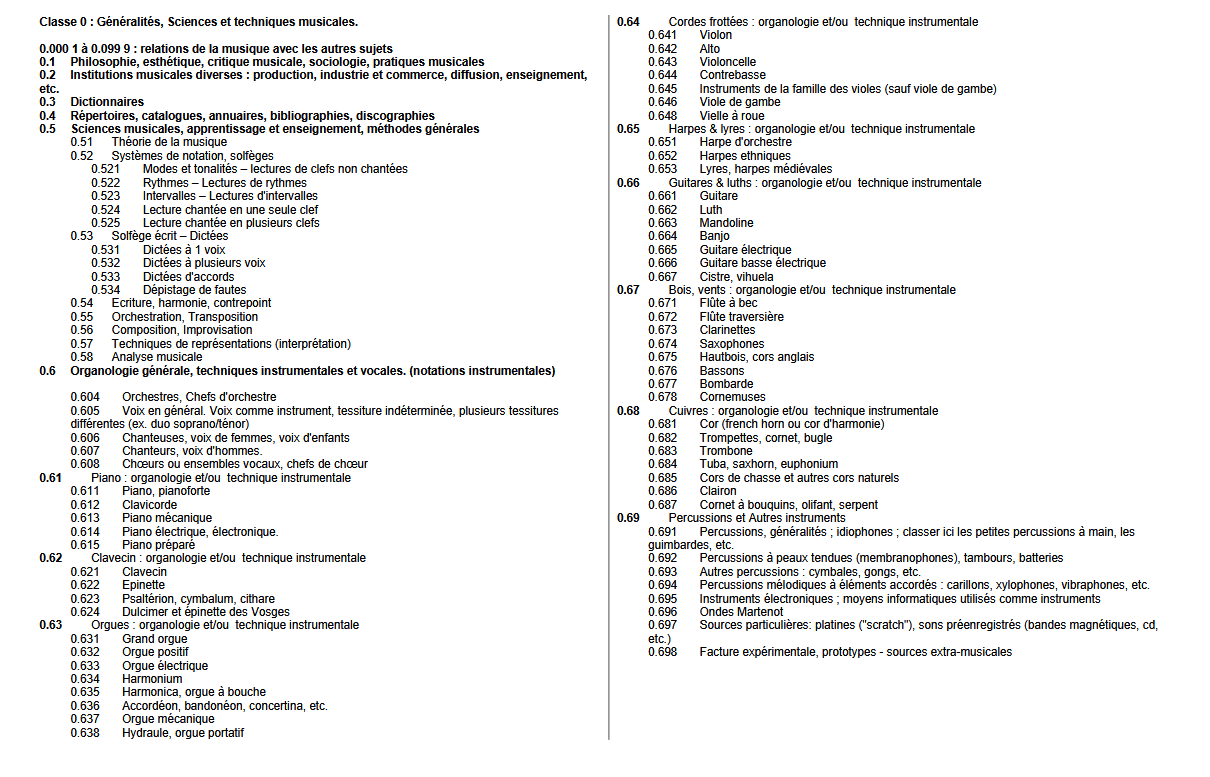
\includegraphics[width=0.6\textwidth]{partie2/images_partie2/images_chapitre4/PCDM4.png}
	\caption{Exemple pour la 1ère classe du Principe de Classement des Documents Musicaux}
\end{figure}

 Par ailleurs, le catalogage des documents musicaux présente des particularités.Lorsque Laurence Karpp-Lahmaidi rédige son mémoire, le modèle FRBR (\textit{Functional Requirements for Bibliographic Records}, ou Spécifications fonctionnelles des notices bibliographiques) n'était pas encore généralisé en France et les documents musicaux faisaient figure de proue dans l'adoption de ce modèle. Le projet ANR Doremus (\textit{Doing Reusable Music Data}), initié en 2014 par la BnF, Radio France et la Philharmonie de Paris a d'ailleurs joué un rôle fondamental dans l'adaptation des modèles de données FRBR/LRM aux spécificités de la musique. En reliant les oeuvres avec leurs interprétations et leurs enregistrements, donnant lieu à des manifestations physiques et numériques, Doremus permet de dépasser les limites des catalogues généralistes non adaptés à la musique et ses complexités (notamment au niveau des transcriptions, enregistrements...). Aujourd'hui, le modèle FRBR a été refondé et a évolué depuis 2017 vers le modèle orienté entité IFLA-LRM (\textit{ International Federation of Library Associations and Institutions - Library Reference Model}). Cela a permis de corriger certaines limites de FRBR, particulièrement problématiques pour la musique. 

Si les fonds patrimoniaux spécialisés en musique font l'objet d'un traitement particulier, mobilisant un réseau d'experts, les sections musique des bibliothèques requièrent également une attention particulière après le bouleversement de la dématérialisation des supports qui les a pleinement touchées. 
A l'heure des plateformes de streaming musical, la bibliothèque fait face à un bouleversement majeur au niveau de ses collections musicales : le nombre d'emprunts de CD chute drastiquement. Sans approfondir quantitativement ce phénomène, analysé par l'élève-conservateur Amandine Pluchet, dans son mémoire de 2012\footnote{Pluchet (Amandine), Les évolutions des sections musique des bibliothèques municipales depuis l’arrivée d’internet, mém. d'étude de conservateur des bibliothèques, dir. X. Galaup, Villeurbanne, Enssib, 2013, 99 p., dactyl. [en ligne], [réf. du 19 juin 2026].} et par Mélanie Lecouteux\footnote{Lecouteux (Mélanie), Nouvelles pratiques professionnelles en section musique, mém. d'étude, dir. C. Paganelli, Montpellier, Université Paul Valéry, 2022. 110 pages.}, nous donnerons ici simplement les grandes tendances des nouvelles pratiques en section musique en bibliothèques. \\

A la suite de la dématérialisation des pratiques musicales, la politique d'acquisition des bibliothèques évolue. Ces dernières doivent proposer une \enquote{offre de collections hybride}(Amandine Pluchet). Même si le modèle de la discothèque de prêt, en vogue dans les années 1960 s'essoufle, il est important de garder une collection physique aux côtés de ressources numériques. 
En effet, le constat d'Amandine Pluchet dans son mémoire est parlant : 
\begin{quotation}
	{A l’heure d’internet et de la musique en ligne, il est plus que
	jamais inconcevable de limiter l’espace musique d’une médiathèque à la seule
	dimension d’une discothèque de prêt. La musique doit s’exprimer dans sa
	diversité, au cœur d’un ensemble de supports aussi bien sonores qu’imprimés:
	CDs et autres enregistrements numériques, mais aussi monographies, et
	périodiques sans oublier les supports destinés aux pratiques amateurs, tels que	partitions et méthodes
	}
\end{quotation}
 Cette politique doit s'effectuer au niveau de l'acquisition, d'une part, qui représente la diversité des supports d'écoute, au moyen d'abonnements à des ressources numériques et d'une veille sur les supports patrimoniaux tels que les vinyles (qui suscitent l'engouement des usagers) et d'autre part au niveau de la médiation musicale. En effet, la politique documentaire ne se limite pas aux acquisitions. Les documents musicaux méritent de faire l'objet d'une programmation culturelle active. 
Par exemple, la bibliothèque patrimoniale  de Dijon, qui conserve un manuscrit musical médiéval, a organisé le 23 avril 2026 un atelier de recherche en partenariat avec l'université de Lausanne et la Haute-Ecole de Musique de Genève. Sur le thème \enquote{Voir, lire, écouter le chansonnier de Dijon}, le public a pu profiter d'un  atelier de recherche suivi d'une visite guidée de la bibliothèque avec une présentation du manuscrit puis d'un concert donné par les étudiants de la HEM. 
En section musique de bibliothèque, les dispositifs de médiation peuvent prendre la forme de borne d'écoute, d'équipements en MAO (Musique Assistée par Ordinateur) avec atelier d'initiation à la prise en main\footnote{Voir à ce sujet le mémoire d'Amandine Pluchet : Pluchet (Amandine),\textit{Les évolutions des sections musique des bibliothèques municipales depuis l’arrivée d’internet}, mém. d'étude de conservateur des bibliothèques, dir. X. Galaup, Villeurbanne, Enssib, 2013, 99 p., dactyl. [en ligne], [réf. du 19 juin 2026], page 61}, ou encore de sélections \enquote{coups de coeur} associées à des concerts dans la bibliothèque. 



\subsection*{Un exemple de charte des collections, la charte des ressources de LaDocumenta.eu}
\label{subsection:Un exemple de charte des collections, la charte des ressources de LaDocumenta.eu}

Appliquées aux bibliothèques d’orchestre, bibliothèques singulières parmi les bibliothèques musicales, ces contraintes d’acquisition et de traitement des collections musicales gagnent à être encadrées par des outils régissant la politique documentaire spécialisée d’une telle bibliothèque.  
Dans le cadre de l'amélioration de la plateforme LaDocumenta.eu, c'est-à-dire la construction de sa nouvelle version (V2) opérée par l'entreprise Reveality.io, il s'est avéré indispensable de réfléchir à l'élaboration d'une \enquote{charte des ressources} de la plateforme. Cet exercice résulte en réalité d'une demande de livrable que le consortium LaDocumenta se doit de fournir au fonds européen qui la soutient, à savoir le programme Europe Creative. C'est dans cet objectif que j'ai été amenée à produire, lors de mon alternance à la bibliothèque de l'orchestre \textit{Insula Orchestra} en tant que chargée de mission LaDocumenta, un pré-livrable\footnote{Ce livrable est consultable dans le volume d'annexes de ce mémoire, sous le titre : Livrable 1 : Charte des ressources de LaDocumenta.eu, pages 4 à 14.} prenant la forme d'une charte des collections. 
Ce livrable se situe donc au coeur de la politique documentaire de la plateforme LaDocumenta.eu. \\
Comme nous l'avons vu, la charte des collections est l'un des outils clés de la politique documentaire.
\begin{quotation}
La charte des collections définit la politique documentaire générale de l’établissement. Elle présente l’organisation de la bibliothèque et en définit les objectifs généraux (supports, secteurs documentaires, critères de choix ou d’exclusion, règles d’élimination ou de conservation, traitement des suggestions ou des dons, etc.). C’est un document interne, porté par la direction et obligatoirement validé par la tutelle, mais qui peut aussi être communiqué au public. C’est un outil destiné à durer plusieurs années, qui doit donc être ré-évalué régulièrement\footnote{Définition issue du groupe Poldoc de l'Association des bibliothécaires de France (ABF):\url{https://www.poldoc.abf.asso.fr/boite-a-outils/}.}.
\end{quotation}

Elle régit les pratiques \enquote{des secteurs documentaires, les supports, les critères de choix et d'exclusion, les règles d'élimination et de conservation ainsi que le traitement des suggestions des adhérents, des dons et des échanges\footnote{Henard (Charlotte), \textit{La politique documentaire, de quoi parle-t-on et comment faire ?}, support de cours de l'ABF, Toulouse, Médiad'Oc, 2024-2025.}}.
La particularité de la charte des collections de LaDocumenta.eu consiste en la matérialité numérique de cette bibliothèque. C'est pour cette raison qu'il a été décidé d'appeler ce document une \enquote{charte des ressources}, en référence aux ressources numériques qui la composent. 

Sur les conseils de la directrice de la bibliothèque de l'Ecole Nationale des Chartes, Camille Degez-Selves, j'ai pris connaissance de la charte documentaire de l'ENSSIB, validée en février 2026 et publiée en avril, qui a été reprise pour construire le plan de la charte des ressources de LaDocumenta.eu\footnote{Pour voir la charte des ressources de LaDocumenta.eu, consulter le volume d'annexes portant sur les livrables technique de ce mémoire, il s'agit du 1er livrable, intitulé \enquote{Charte des ressources de LaDocumenta.eu}, page 5}.
En me référant à la charte documentaire de l'ENSSIB (Ecole Nationale Supérieure des Sciences de l'Information et des Bibliothèques)\footnote{Voir la charte documentaire 2026 de l'ENSSIB à cette adresse : \url{https://www.enssib.fr/sites/enssib.fr/files/inline-files/Charte-documentaire-Enssib-2026.pdf}}, j'ai choisi d'élaborer la charte des collections de LaDocumenta.eu en suivant ce plan : 
\begin{figure}[H]
	\centering
	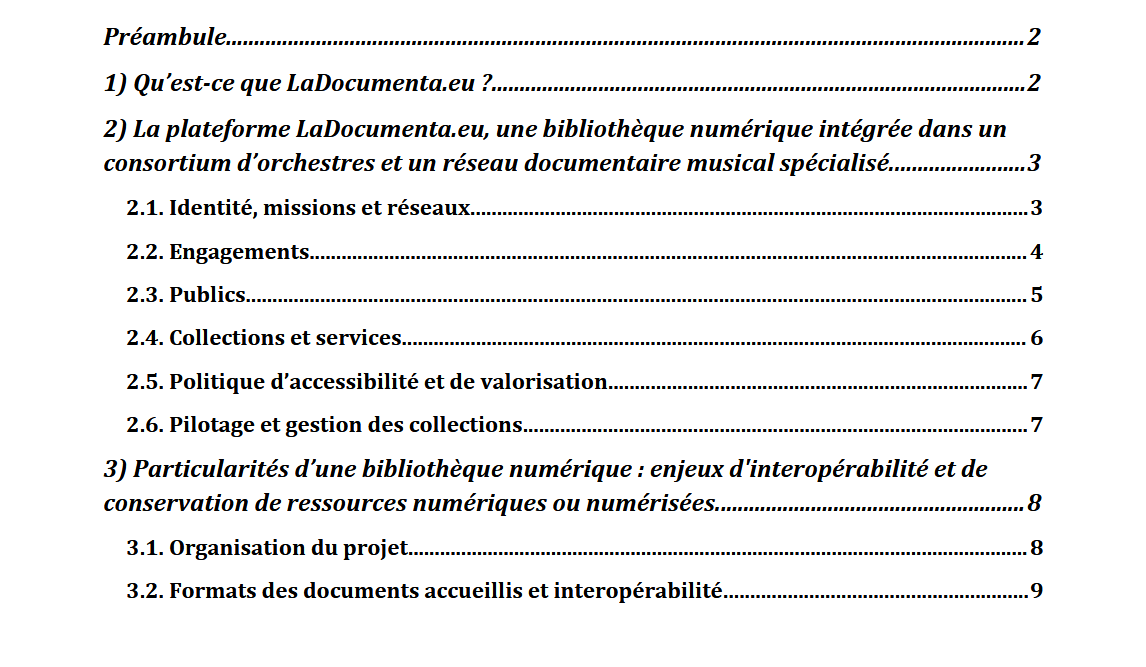
\includegraphics[width=0.9\textwidth]{partie2/images_partie2/images_chapitre4/plan_charte_ressources.png}
	\caption{Capture d'écran du plan du pré-livrable de charte des ressources de LaDocumenta.eu}
\end{figure}

Il a été bénéfique de réutiliser les grandes idées de la charte documentaire de l'ENSSIB pour l'adapter au cas de LaDocumenta.eu. 

\begin{itemize}
	\item Le \textbf{préambule} a permis d'introduire aux futurs lecteurs l'enjeu d'une charte documentaire. Il permet d'affirmer l'utilité du document tout en en précisant l'utilisation et les conditions de publication (comme la validation préalable du conseil scientifique du consortium)
	\item La \textbf{première partie} a permis de présenter clairement les objectifs de LaDocumenta.eu, à la fois consortium et plateforme, base de données et bibliothèque numérique, site internet du consortium et interface privée des membres du consortium, en remplacement d'un éventuel Système de Gestion de Bibliothèque (SIGB) comme ceux des logiciels PMB. 
	Cette partie présente également les enjeux de la plateforme, qui seront détaillés ensuite. 
	\item La \textbf{deuxième partie} explicite la différence entre une politique documentaire généraliste et une politique doublement spécialisée comme celle de LaDocumenta.eu, avec d'une part la spécialité musicale, et d'autre part le support numérique.
	
	\begin{itemize}
		\item Le premier point s'appuie sur un entretien mené avec l'équipe de développeurs de la plateforme : l'entreprise Reveality.io\footnote{Entretien avec Maxime Touroute, développeur de LaDocumenta.eu, mené le 1er juillet 2026, avec contributions écrites de Marc Karassev, également développeur de LaDocumenta.eu. La grille d'entretien est consultable en annexes.} pour avoir un socle de connaissances solide sur les précisions techniques de la plateforme. L'objectif est d'expliquer simplement le fonctionnement de la plateforme. 
		Il concerne également les missions et aspirations futures de la plateforme.
		
		\item Le deuxième point porte sur les engagements de la plateforme. L'idée de ce développement est de s'inscrire dans le réseau européen Europe creative, pour lequel LaDocumenta.eu a été lauréate et d'affirmer les convictions du consortium, dans une continuité avec les priorités européennes des campagnes de financement. 
		
		\item Le troisième point présente les publics de la plateforme en les regroupant dans des catégories. Ces catégories ont été réutilisées ensuite pour élaborer le 3e livrable\footnote{Voir à ce propos le 3e livrable du volume des annexes techniques : \enquote{Usages de la Documenta.eu et scénario d'utilisation de l'IA} de ce mémoire, portant sur les usages IA de la plateforme.} 
		
		\item Le quatrième point constitue le coeur de la charte documentaire de LaDocumenta.eu puisqu'il informe le lecteur sur le corpus de la plateforme. Dans ce point est expliqué l'organisation même des ressources de la plateforme, suivant le découpage des phases d'une production musicale (pré-production, production, concert et post-production\footnote{Ce découpage en phases de production, au sujet de l'organisation des ressources, est l'oeuvre de Kai Kopp, directeur du comité scientifique du consortium}).
		\item Le cinquième point concerne l'accessibilité et la valorisation des collections. Après avoir rappelé l'accessibilité, fidèle principe d'ouverture des bibliothèques. Cette section précise les modalités d'accès, nécessairement adaptées en raison du caractère numérique de la plateforme.\\ 
		Il y a deux points d'attention dans cette section : la consultation et le téléchargement des ressources ainsi que la gestion des ressources sous droits.\\
	Ce dernier point, grisé, n'a pas pu être traité à cet état d'avancement de ce pré-livrable. En effet, ce questionnement convoque des considérations de droit de la propriété intellectuelle qui seront abordées en conseil scientifique prochainement et qui n'avaient pas été tranchées ni lors de l'élaboration de ce livrable, ni à mon départ de stage. Il semblerait par ailleurs que cette question devrait faire l'objet d'une réflexion à part entière dans les projets de financement suivants. Un profil de doctorant en droit de la propriété intellectuelle, travaillant sur les questions de droit en contexte numérique, a été évoqué par l'IreMus, partenaire scientifique de la plateforme. \\
	J'ai toutefois proposé une ébauche de réflexion dans le livrable et indiqué des références bibliographiques à mes responsables. Ensemble, nous avons convenu que ces considérations juridiques poseraient majoritairement problème quant à la communicabilité des ressources. Nous pouvons donc dès à présent envisager les questionnements qui seront à l'ordre du jour des réflexions du comité scientifique, notamment en regard des implications UX de la plateforme en présence d'un document sous droits. Nous pouvons donc supposer que, comme dans Gallica, une ressource sous droits pourrait ne pas apparaître sur la plateforme utilisateur mais seulement sur la plateforme de l'orchestre contributeur. L'usager intéressé pourrait être invité à consulter en présentiel la ressource à la bibliothèque de l'ensemble contributeur, sur un intranet et sans moyen de télécharger la ressource. L'usager pourrait également se voir proposer un fichier filigrané rendant impossible la lecture de la ressource complète, lui permettant toutefois de pouvoir prendre connaissance de l'incipit de la ressource par exemple. 
		\item Le sixième point porte sur le pilotage et la gestion des collections. Il est constitué de trois thématiques que sont : l'administration de la plateforme, la collecte et le dépôt des ressources de la plateforme ainsi que la conservation des ressources de la plateforme. Pour ce sixième point, lui aussi grisé, il ne m'a pas été possible non plus de proposer un texte car les critères d'admission d'une plateforme, les modalités de collecte ainsi que la politique de pilotage des collections n'avaient pas encore fait l'objet de directives de la part du comité scientifique. Comme pour les questions juridiques, j'ai indiqué les principales thématiques qui devraient être abordées prochainement, comme les critères de sélection des ressources (qualité, rareté...), la politique en cas de doublon, ou encore les enjeux de pérennité des collections numériques mais il était impossible à ce stade de proposer une réflexion de mon côté, sans concertation avec le comité scientifique. 
	\end{itemize}
\item La \textbf{troisième partie} sera détaillée dans le chapitre suivant car elle porte davantage sur les enjeux numériques de standardisation et d'intéropérabilité que sur l'élaboration d'une charte des collections. La problématique des référentiels, non abordée dans ce chapitre illustre en effet les questionnements que pose la plateforme au sujet de la standardisation des données et de l'intéropérabilité.  Après avoir détaillé la politique documentaire de la plateforme LaDocumenta.eu dans ce quatrième chapitre, l'on s'attelera à présenter les enjeux de la standardisation des données des plateformes numériques dans un objectif de construire l'intéropérabilité des données musicales. 	
\end{itemize}	

	\chapter{La standardisation comme prérequis à l'interopérabilité}
L'interopérabilité des données, recherchée par les plateformes numériques à l'instar de LaDocumenta.eu, suppose un cadre méthodologique de structuration et de normalisation rigoureuse des données. Appliquée aux bibliothèques spécialisées que représentent les bibliothèques d'orchestre, cette exigence technique est la condition pour que les documents patrimoniaux (conducteurs annotés, matériel d'orchestre, etc.) deviennent des données de recherche exploitables et interopérables pour nourrir l'interprétation historiquement informée. La transformation de ces sources matérielles en ressources interopérables permet dès lors aux musicologues, musiciens et chercheurs de disposer d'outils pour documenter et restituer les pratiques historiquement informées au moyen de portails documentaires interrogeables entre eux. Pour comprendre la portée de cette transformation, il convient d'étudier le passage du signalement traditionnel aux métadonnées structurées pour analyser la capacité des standards du web de données à traiter la complexité des données musicales. Cette démarche correspond à un objectif d'interaction et de réutilisation des données à l'échelle européenne puis internationale.

\subsection*{Du signalement traditionnel aux métadonnées structurées}

En bibliothéconomie, il est d'usage d'élaborer une politique documentaire pour régir la vie de la bibliothèque, que ce soit au niveau de l'organisation ou de la médiation des collections. Dans une plateforme numérique, la politique de gouvernance des données, qui cadre et pilote le traitement de la donnée, remplit le même rôle. Ainsi, on observe une transformation des pratiques en bibliothèques allant d'un signalement traditionnel à une réflexion centrée sur les données.

\subsubsection*{De la fiche bibliographique aux métadonnées structurées : \enquote{La bibliothèque face au monde des données}\footnote{Mesguich (Véronique), \textit{Les bibliothèques face au monde des données}, Presses de l’enssib, 2023, \url{https://doi.org/10.4000/books.pressesenssib.17686}.}}

Comme nous l'avons vu dans le premier chapitre, la transformation numérique des bibliothèques a profondément reconfiguré leurs modes d'accès et leurs supports.

Le signalement — entendu comme \enquote{la description de documents constituant un fonds pour en assurer la diffusion, le rendre accessible à la recherche et en favoriser la consultation}\footnote{Définition du vocabulaire de l'ADBU (Association des directeurs et personnels de direction des bibliothèques universitaires et de la documentation), 2024 : \url{https://adbu.fr/info-doc-vocabulaire-notions-de-base/signalement}.} — était historiquement voué à la description interne. Le bouleversement de l'informatisation a eu comme répercussion, dans le monde des bibliothèques, de transposer la notice cartonnée vers des formats informatiques métiers comme les formats MARC (\textit{Machine Readable Cataloguing}), ou propriétaires comme des tables relationnelles de SIGB (Système intégré de gestion de bibliothèque) à l'image d'Aloès du logiciel Archimed\footnote{Aloès est un SIGB proposé par la société Archimed.}.

Toutefois, la généralisation du web et la transformation des usages et attentes des usagers ont modifié l'accès à l'information. Après un signalement d'ouvrage dans un catalogue local, les usagers attendent maintenant un accès direct aux données. Les institutions voient donc leurs méthodes évoluer pour que leurs notices sortent des silos applicatifs des catalogues et intègrent ainsi le web de données.

L'objectif est de produire des \enquote{données structurées} :
\begin{quotation}
	[Ce sont des] éléments calibrés saisis dans les différents champs de bases de données\footnote{Définition de Marie-Anne Chabin dans le \textit{Nouveau glossaire de l'archivage} (2010) : \url{https://www.arcateg.fr/wp-content/uploads/2017/03/Nouveau_glossaire_de_l_archivage.pdf}.}. Les données structurées sont contrôlées par des référentiels, et leur structure permet leur interprétation ainsi que leur traitement par des machines. Elles peuvent être stockées dans des bases de données relationnelles, interrogeables par des langages de requêtes structurées (SQL ou \textit{Structured Query Language}). Les données structurées se trouvent également dans des fichiers aux formats XML, CSV ou JSON\footnote{Mesguich (Véronique), \enquote{Chapitre 1. Qu’est-ce qu’une donnée ? Formats, standards, cycle de vie des données…}, dans \textit{Les bibliothèques face au monde des données}, Villeurbanne, Presses de l’enssib, \url{https://doi.org/10.4000/books.pressesenssib.17761}.}.
\end{quotation}

Cela suppose une réflexion sur les métadonnées bibliographiques manipulées dans les catalogues de bibliothèques. Ces métadonnées doivent se muer en données visibles, interopérables et réutilisables pour d'autres institutions culturelles et patrimoniales.

En effet, les notices de bibliothèques, enfermées dans des silos de données — ensembles isolés de données qui empêchent leur partage entre les différents services, systèmes et unités commerciales\footnote{Définition d'IBM (\textit{International Business Machines Corporation}) : \url{https://www.ibm.com/fr-fr/think/topics/data-silos}.} — organisaient leurs métadonnées en blocs avec des identifiants locaux les rendant invisibles pour un usage externe.

Souffrant d'une \enquote{double invisibilité}\footnote{Mesguich (Véronique), \textit{op. cit.}}, les catalogues de bibliothèques ont tendance à se composer d’URL complexes, non indexées par les moteurs de recherche, ce qui les relègue dans le \enquote{web profond}.

Les catalogues doivent alors évoluer vers de nouvelles formes de notices dont les données sont des entités autonomes reliées entre elles (auteur, œuvre, etc.) reposant sur des URI (\textit{Uniform Resource Identifier}) accessibles sur le web.

Pour une politique documentaire adaptée au web, il est nécessaire que chaque entité du catalogue devienne une ressource indépendante avec un identifiant unique. Cette mutation, à l'œuvre en ce moment dans les bibliothèques, est l’enjeu du programme national de la Transition bibliographique, un modèle de structuration informatique basé sur les standards du web sémantique. Ce programme, lancé en 2014 par le Comité stratégique bibliographique (CSB), accompagne le passage historique des formats standards MARC — centrés sur la description d’un document unique — vers le modèle conceptuel international IFLA-LRM (\textit{Library Reference Model}). Ce nouveau modèle divise l’information en structurant le catalogue autour du réseau d’entités OEMI (Œuvre, Expression, Manifestation, Item) reliées entre elles. En France, cette démarche s’appuie sur la rédaction du nouveau code de catalogage national RDA-FR ainsi que sur l’évolution du format d’échange vers UNIMARC ER (Entités-Relations).

\begin{figure}[H]
	\centering
	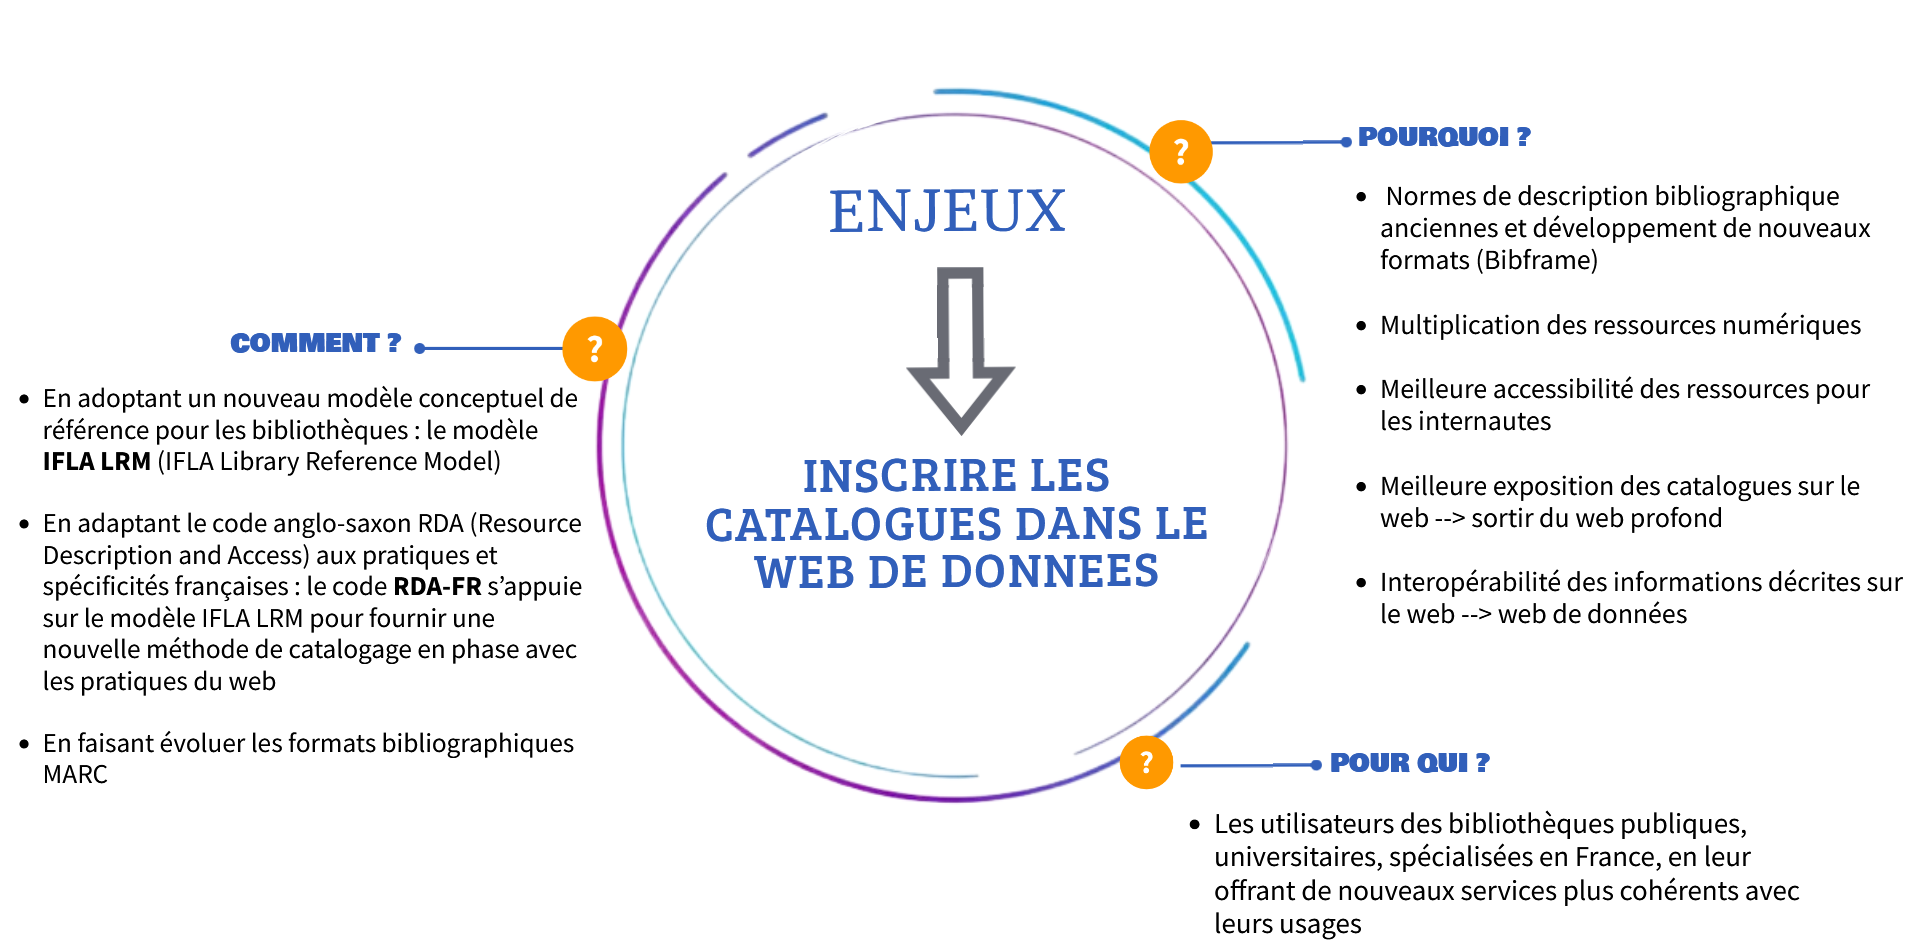
\includegraphics[width=0.8\textwidth]{partie2/images_partie2/images_chapitre5/transition_bibliographique.png}
	\caption{Schéma de la Transition bibliographique (\url{https://www.transition-bibliographique.fr/enjeux/}).}
\end{figure}

Après dix ans de réflexion sur ces normes de formation et de sensibilisation des bibliothécaires, la Transition bibliographique entre dans une phase d’aboutissement et d’implémentation. En témoignent le déploiement de NOEMI, le nouvel outil de catalogage nativement fondé sur les normes LRM et RDA-FR à la BnF, et la préparation du renouvellement du système de gestion des métadonnées de l’Abes.

La Transition bibliographique, dans sa phase d’implémentation, est un enjeu important pour les bibliothèques qui se doivent d’intégrer progressivement ces nouveaux outils dans leur politique documentaire.

\subsubsection*{De la politique documentaire à la gouvernance des données}

Dans un contexte numérique, nous l'avons vu, les bibliothèques expérimentent de nouveaux outils pour mettre en œuvre leur politique documentaire. Pensée non comme le remplacement mais comme le prolongement de la politique documentaire, la gouvernance des données en est un exemple marquant.

La politique documentaire s'articule autour du cycle de vie du document, physique ou numérique, qui se compose en bibliothèque des opérations de sélection, d'acquisition, de traitement, de conservation et de désherbage. Les bibliothèques, dans leur volonté de produire des données structurées, élargissent donc leur politique documentaire à la politique de gouvernance des données.

\begin{quotation}
	La gouvernance des données est la stratégie qui se compose de normes, principes et règles régissant divers types de données au-delà de la gestion purement technique. Elle s'applique à la gestion des données, leur accès, leur stockage, leur mise à jour et leur consommation au sein d’une organisation afin d’en optimiser la valeur et l’efficacité des traitements et des expositions. C'est une stratégie dont le but est d’assurer l’efficacité des traitements liés à la donnée pour assurer son exploitation\footnote{Définition de Lauryne Lemosquet dans le cadre du cours donné aux étudiants de master Technologies Numériques Appliquées à l'Histoire à l'École nationale des chartes.}.
\end{quotation}

La mise en œuvre de la gouvernance des données est un ensemble d'opérations regroupées sous le nom de traitement de la donnée. Comme le document, la donnée a un cycle de vie. Il se compose de la création, du traitement, de l'analyse, de la conservation, de l'accès et de la réutilisation de la donnée\footnote{Voir l'encadré \enquote{Les six étapes du cycle de vie de la donnée}, dans Mesguich (Véronique), \enquote{Chapitre 1. Qu’est-ce qu’une donnée ? Formats, standards, cycle de vie des données…}, \textit{Les bibliothèques face au monde des données}, Villeurbanne, Presses de l’enssib, \url{https://doi.org/10.4000/books.pressesenssib.17761}.}.

Parmi ces opérations, \enquote{l’intégration de la donnée} est une étape clé. Dans le système d’information (SI), les données viennent de sources multiples avec des formats variables. L’opération d’intégration consiste en l’unification de ces sources selon un modèle conceptuel destiné à alimenter des bases de données fiables et interopérables (le \textit{back-end}).

Pour aboutir à cette transition de données brutes à des (méta)données structurées, la démarche d’intégration de la donnée doit répondre à des exigences précises de la gouvernance des données\footnote{Items soulignés par Lauryne Lemosquet dans le cadre du cours donné aux étudiants de master Technologies Numériques Appliquées à l'Histoire à l'École nationale des chartes.} :
\begin{itemize}
	\item \enquote{Un processus de normalisation et de rationalisation orienté vers la qualité}\footnote{\textit{Idem}} ;
	\item \enquote{Une parfaite maîtrise de la sémantique et des règles de gestion des données manipulées}\footnote{\textit{Idem}} ;
	\item \enquote{Une bonne gestion des référentiels, incluant une vérification constante de leur intégrité}\footnote{\textit{Idem}}.
\end{itemize}

Cette politique de gouvernance des données vise à transformer des données à la qualité variable en données traitées et organisées. Dans cette recherche, les référentiels, thésaurus et ontologies constituent un socle sémantique et technique important sur lequel repose l'intégration des données. Si la gouvernance des données ne se limite pas à l'interopérabilité des données, ces outils de référentiels facilitent toutefois l'interopérabilité des données et la mise en œuvre des normes de la politique de gouvernance des données.

\subsubsection*{Référentiels, thésaurus, ontologies : poser les bases de l'interopérabilité}

Les référentiels permettent de poser les fondations de l’interopérabilité. En effet, ils facilitent la cohérence des valeurs attribuées aux métadonnées et garantissent un contrôle du vocabulaire dans les systèmes d’information (SI). Les référentiels sont donc des hubs de données censés connecter les bases de données entre elles au sein d’une même institution ou entre institutions culturelles et patrimoniales différentes.

Pour poursuivre leur objectif d’interopérabilité, les bibliothèques ont recours aux thésaurus, qui sont des outils de structuration. Répondant aux normes internationales ISO 25964-1:2011\footnote{Détails sur la norme ISO 25964-1:2011 : \url{https://www.iso.org/fr/standard/53657.html}.} et ISO 25964-2:2013\footnote{Détails sur la norme ISO 25964-2:2013 : \url{https://www.iso.org/fr/standard/53658.html}.}, les thésaurus fonctionnent ainsi : un concept est exprimé par un terme préféré, les autres termes non descripteurs étant considérés comme des synonymes, par langue. Les concepts sont ensuite reliés à d’autres concepts\footnote{Définition d'Emmanuelle Bermès, donnée dans le cadre d’un cours aux étudiants du master TNAH.}. Un thésaurus s’organise donc selon une modélisation conceptuelle rigoureuse :

\begin{itemize}
	\item \textbf{L’expression univoque des concepts :} chaque concept est exprimé par un (et un seul) terme descripteur par langue (par exemple le concept de \textit{Piano}) ;
	\item \textbf{La gestion des synonymes :} les variantes lexicales, les formes rejetées, les abréviations ainsi que les évolutions chronologiques sont des termes non descripteurs (par exemple, en reprenant le concept de \textit{Piano} : \textit{pianoforte}, \textit{piano à queue}, \textit{Klavier}, \textit{Pno.}) ;
	\item \textbf{Les relations avec d’autres concepts :}
	\begin{itemize}
		\item \textit{Relations hiérarchiques et polyhiérarchiques :} des relations structurées selon des logiques génériques, partitives ou d’instanciation (par exemple la hiérarchie \textit{Instrument de musique} $\gg$ \textit{Instrument à cordes} $\gg$ \textit{Piano}, ou la polyhiérarchie reliant \textit{Instrument à clavier} et \textit{Instrument à cordes frappées} au \textit{Piano}) ;
		\item \textit{Relations associatives :} des relations de liens thématiques, fonctionnels et contextuels (par exemple des liens d'agent/action ou d'association entre \textit{Piano} et des termes techniques associés comme \textit{Pédale douce}, ou encore des noms de marque comme \textit{Steinway \& Sons}).
	\end{itemize}
\end{itemize}

Dans le web sémantique, dont l’objectif est de \enquote{partager, enrichir les données de manière structurée pour donner du sens et améliorer la pertinence des recherches}\footnote{Mesguich (Véronique), \enquote{Chapitre 2. Bibliothèques et web de données}, dans \textit{Les bibliothèques face au monde des données}, Villeurbanne, Presses de l’enssib, 2023, \url{https://doi.org/10.4000/books.pressesenssib.17761}.}, cette structure des thésaurus s’incarne dans le standard SKOS (\textit{Simple Knowledge Organization System}), développé par le W3C (Le World Wide Web Consortium)\footnote{Le W3C élabore des normes et des lignes directrices pour aider chacun à construire et à profiter d’un Web basé sur les principes d’accessibilité, d’internationalisation, de confidentialité et de sécurité : \url{https://www.w3.org/}}. SKOS est le standard permettant de formaliser les thésaurus en graphes exploitables par les machines. Il s’agit d'une ontologie, c’est-à-dire un vocabulaire RDF (\textit{Resource Description Framework}), destinée à décrire des thésaurus. RDF sert à exprimer l’information par des phrases simples appelées triplets. Ces triplets se composent d’un sujet, d’un prédicat et d’un objet :

\begin{itemize}
	\item \textbf{Le sujet :} la ressource décrite, identifiée par une URI (\textit{Uniform Resource Identifier}) ;
	\item \textbf{Le prédicat :} ce qui est dit à propos du sujet (le type de relation qui lie le sujet à l'objet) ;
	\item \textbf{L'objet :} l'entité sur laquelle porte la relation (une autre ressource identifiée par une URI ou une valeur littérale).
\end{itemize}

Dans les triplets, les concepts sont identifiés par des identifiants pérennes comme les URI (\textit{Uniform Resource Identifier}), c'est-à-dire des \enquote{unités de base du web sémantique [qui] sont comme les mots d’un langage [dont RDF serait la grammaire]}. L'ARK (\textit{Archival Resource Key}) est un schéma d'identifiant pérenne (qui s'exprime sous forme d'URI pérenne) utilisé notamment pour les ressources de la BnF afin de citer de façon stable les ressources vers d'autres pages\footnote{Mesguich (Véronique), \enquote{Chapitre 2. Bibliothèques et web de données}, \textit{Les bibliothèques face au monde des données}, Presses de l’enssib, 2023, \url{https://doi.org/10.4000/books.pressesenssib.17741}.}.

Les relations entre concepts sont codifiées par des propriétés précises : \texttt{skos:prefLabel} (terme privilégié), \texttt{skos:altLabel} (synonymes et variantes), \texttt{skos:note} (note d'application précisant le périmètre d'emploi), ainsi que les relations hiérarchiques (\texttt{skos:broader}, \texttt{skos:narrower}) et associatives (\texttt{skos:related}).

Les triplets permettent de transformer l'information en graphe de données. Ainsi, de l'identifiant pérenne à la modélisation de l'ontologie, la gouvernance des données rend la donnée interopérable.

Le standard SKOS modélise les données sous forme de graphe de connaissances, faisant des référentiels des piliers de l’interopérabilité grâce à l’alignement des données.

Le web sémantique distingue principalement deux niveaux de correspondance selon la nature des objets alignés :

\begin{itemize}
	\item \textbf{La propriété d’identité stricte \texttt{owl:sameAs} :} issue de l'ontologie OWL (\textit{Web Ontology Language}, langage standardisé par le W3C pour la formalisation des ontologies), cette propriété affirme une identité stricte entre deux ressources du web désignant la même entité du monde réel ;
	\item \textbf{La propriété d’équivalence \texttt{skos:exactMatch} (ou \texttt{skos:closeMatch}) :} il s’agit d’une relation d’équivalence entre des concepts de thésaurus différents, qui n’affirme pas l’identité stricte des entités.
\end{itemize}

Le projet data.bnf.fr est \enquote{l’un des premiers exemples européens de portail orienté entité}\footnote{Bermès (Emmanuelle), \enquote{Web de données et bibliothèques : l’évolution du modèle d’agrégation des données}, \textit{I2D – Information, données \& documents}, 2016/2 (vol. 53), p. 37, \url{https://www.cairn.info/revue-i2d-information-donnees-et-documents-2016-2-page-37.htm}.}. En utilisant les référentiels, data.bnf.fr regroupe autour de fiches virtuelles (les entités \textit{Auteur}, \textit{Œuvre} et \textit{Thème}) des données dispersées dans différents catalogues (la notice d’autorité, le catalogue général, Gallica) pour attribuer à chaque entité une URI pérenne (un lien ARK).

D’après Emmanuelle Bermès, \enquote{son originalité est de proposer à la fois des pages web destinées aux internautes et des données brutes en RDF reliées avec d’autres jeux de données (DBpedia, VIAF, Europeana, par exemple)}\footnote{Bermès (Emmanuelle), \textit{ibid.}}. Data.bnf.fr peut être vu comme un hub d'entités qui lie ses notices d'autorité (avec la propriété \texttt{owl:sameAs}) à des bases externes (comme Wikidata ou IdRef), tout en s'appuyant sur les propriétés SKOS pour aligner ses langages d'indexation (comme RAMEAU) avec d'autres thésaurus internationaux. Cela permet aux données de la BnF de sortir de leur silo institutionnel pour s'insérer pleinement dans le web de données\footnote{Présentation du projet sur le site officiel de la BnF : \url{https://www.bnf.fr/fr/databnf.fr}.}.

Il apparaît dès lors que la standardisation et l’alignement de ces référentiels constituent des outils indispensables à la constitution d’un web de données patrimoniales.

Pour une plateforme appliquée aux bibliothèques d’orchestre comme LaDocumenta.eu, ce cadre normatif permet d’extraire les collections spécialisées de leurs silos pour les transformer en données de la recherche et de l’interprétation musicale interopérables.




\subsection*{L'interopérabilité des données musicales}

Le web de données aussi appelé\textit{ Linked Open Data} a été décrit par Tim Berners-Lee dans la note \enquote{Linked data\footnote{\url{https://www.w3.org/DesignIssues/LinkedData.html}}} en 2006. Il peut s'entendre comme \enquote{l'application des standards et technologies du web sémantique pour échanger et relier les données structurées sur le web\footnote{Mesguich (Véronique), \enquote{Chapitre 2. Bibliothèques et web de données}, \textit{Les bibliothèques face au monde des données}, Presses de l’enssib, 2023, \url{https://doi.org/10.4000/books.pressesenssib.17741}}}.  Si le web de données permet de sortir les (méta)données des silos applicatifs dans lesquels elles sont cachées, les particularités des documents musicaux conservés en bibliothèques musicales et d'orchestre - comme les conducteurs et les parties séparées, annotés ou non, les imprimés et manuscrits musicaux - peuvent être un frein à l'application des normes traditionnelles de catalogage. 

En effet, les ressources musicales ne sont pas adaptées aux notices bibliographiques standards. Les partitions annotées par exemple présentent la spécificité de se composer à la fois d'un texte musical (notation musicale) et d'annotations, écrites à la main, portant sur l'interprétation ou l'effectif musical (comme des coupures, des coups d'archet...) qui sont fondamentales pour la construction de l'interprétation historiquement informée. Cette particularité de contenir deux typologies d'écritures différentes qui ne peuvent être lues par les mêmes outils complique le traitement de ces ressources. 
En effet, la donnée musicale, qu'elle soit physique ou numérique, donne lieu à de multiples expressions d'une même oeuvre. Le traitement bibliothéconomique d'une telle ressource s'avère compliqué car elle chamboule les règles pré-établies concernant la gestion des collections de la bibliothèque. Que faire si la bibliothèque conserve deux éditions strictement identiques d'une même oeuvre mais annotées par deux chefs différents ? L'annotation pouvant être vue en bibliothéconomie traditionnelle comme une dégradation, quelles motivations peuvent encourager les équipes à garder un tel exemplaire, face au stockage limité en magasin ? Si l'ouvrage est gardé mais n'est pas valorisé dans la plateforme numérique de l'orchestre, quel intérêt si l'annotation n'est pas exploitable d'un point de vue de la recherche ? C'est à ce type de questions que tentent de répondre les initiatives de prises en compte des outils numériques spécialisés dans le traitement de la donnée musicale. 

\subsubsection*{La ressource musicale, une ressource complexe adaptée au modèle orienté entité.}

Dans une bibliothèque d'orchestre, un titre d'oeuvre ne peut pas se résumer en une ressource. Il existe tellement de déclinaisons matérielles d'une même oeuvre qu'il peut s'avérer difficile de les individualiser. Le modèle IFLA-LRM offre alors une solution intéressante pour décrire le plus finement possible les ressources musicales. En effet, le modèle IFLA-LRM permet de séparer de manière rigoureuse \enquote{l'Oeuvre}, \enquote{l'Expression}, \enquote{la Manifestation} et \enquote{l'Item}, c'est-à-dire les quatre entités (OEMI) du modèle IFLA-LRM : 

\begin{itemize}
	\item \textbf{L'Œuvre :} la création abstraite (par exemple la \textit{Symphonie $n^o$ 3 en mi bémol majeur}, op. 55 de Beethoven, \textit{L'éroica}) ;
	\item \textbf{L'Expression :} la réalisation intellectuelle ou artistique spécifique, comme une révision par le compositeur, un arrangement pour orchestre réduit ou une version d'époque (par exemple l'expression orchestrale fixée par la première édition de 1806) ;
	\item \textbf{La Manifestation :} l'édition ou le manuscrit matérialisé sous forme de publication (par exemple  le matériel gravé par Breitkopf \& Härtel) ;
	\item \textbf{L'Item :} l'exemplaire physique annoté, contenant des indications précieuses sur l'interprétation (par exemple le conducteur annoté par Laurence Equilbey, lors de la préparation du concert Beethoven qui aura lieu à la Seine Musicale les 25 et 26 septembre 2026).
\end{itemize}


Ces distinctions d'entités sont très précieuses pour documenter l'interprétation historiquement informée de la musique. En effet, la spécificité des données musicales (par exemple : la \textit{Symphonie $n^o$ 3 en mi bémol majeur}, op. 55 de Beethoven), qui peuvent être à la fois \enquote{Oeuvre}, \enquote{Manifestation} et \enquote{Item}, nécessite une précision importante, voire des outils spécialisés. 
Le chercheur musicologue ou musicien est alors à la recherche d'une interaction sémantique entre l'\enquote{Item} (comme des annotations sur la manière d'interpréter une pièce) et le contexte de l'époque. 
Dès lors, les ontologies du web sémantique comme Doremus (Doing Reusable MUSical data), l'extension FRBRoo(\textit{Functional Requirements for Bibliographic Records} orienté objet)/LRMoo , destinés à la description des catalogues musicaux, permettent de préciser ces relations à l'aide de triplets RDF en spécifiant les liens entre les musiciens, leur instrument, les concerts et la documentation des concerts. 

\subsubsection*{Standards d'encodage musicaux et enjeux de numérisation}

L'interopérabilité des données musicales repose, comme nous l'avons vu, sur le rapport entre les métadonnées de description et le contenu musical décrit. Pour construire cette interopérabilité des données musicales, deux standards existent : 

\begin{itemize}
	\item La\textbf{ MEI }(\textit{Music Encoding Initiative}) est un \enquote{système d'encodage de documents musicaux qui rassemble des spécialistes en musicologie, histoire, humanités numériques ainsi que des bibliothécaires. Ce standard XML permet ainsi aux ordinateurs de lire et reproduire la musique notée\footnote{Feustle (Maristella), Intro to MEI. \url{https://works.hcommons.org/records/vbczn-0af28}}}. La MEI permet d'encoder non seulement la musique notée mais aussi l'apparat critique, les \textit{incipit} et les annotations manuscrites à l'endroit précis, à la note ou à la mesure près. Ainsi, un conducteur numérisé en MEI contient des données de recherche interrogeables par des algorithmes (recherche de motifs mélodiques ...)
	
	\item Le protocole \textbf{IIIF} (\textit{International Image Interoperability Framework}) - à prononcer [trois \enquote{i} F]- est un protocole d'exposition et de manipulation d'images haute-définition qui permet de lier les zones d'une image numérisée (par exemple une annotation de chef sur une mesure précise) avec les structures encodées en MEI ou documentées dans un catalogue de bibliothèque, si la MEI est couplée au standard IIIF-AV (Audio-Visuel), il est possible de lier l'image avec un enregistrement sonore.  
\end{itemize}

\subsubsection*{Référentiels spécialisés en musique et alignements internationaux}

Pour permettre aux fonds musicaux des plateformes musicales numériques à l'image de LaDocumenta.eu d'être interopérables à l'échelle européenne, leur alignement aux grands réservoirs de données est fondamental. 
Ces réservoirs de données, à l'image du RISM ou des thésaurus et autorités spécialisées permettent, comme pour les données non spécialisées, de poser les fondations de l'interopérabilité. 

\begin{itemize}
	\item \textbf{Le RISM (\textit{Répertoire International des Sources Musicales})} est le référentiel mondial de description des sources musicales manuscrites et imprimées.
	
	Les bibliothèques musicales spécialisées peuvent solliciter une demande d'attribution d'identifiant RISM, afin d'avoir une reconnaissance de bibliothèque spécialisée, ou de bibliothèque classique à fonds musical remarquable. Par ailleurs, chaque source musicale inscrite au RISM possède également un identifiant RISM. 
	Ainsi, l'attribution d'un identifiant RISM associée à l'alignement des incipits musicaux au moyen du code Plaine \& Easie\footnote{Le code Plaine \& Easie est un \enquote{système d'encodage de notation musicale conçu pour la capture d'incipits mélodiques : courts fragments de notation musicale qui aident à identifier l'œuvre musicale}. Il est développé et entretenu par le RISM (\url{https://plaine-and-easie.info/}).} permet l'identification numérique d'une source musicale.
 
	\item \textbf{Les thésaurus et autorités spécialisés }: l'alignement des noms de compositeurs, d'instrumentistes et de facteurs d'instruments s'appuie sur des référentiels d'autorité comme la GND (\textit{Gemeinsame Normdatei} de la Bibliothèque nationale allemande) ou VIAF, ainsi que sur des vocabulaires contrôlés d'instruments (tels que le thésaurus de l'MIMO -- \textit{Musical Instrument Museums Online}).
\end{itemize}

En associant le modèle IFLA-LRM, l'encodage du format MEI et la mise en réseau par les triplets RDF, le traitement des fonds musicaux des bibliothèques musicales et d'orchestre érige le matériel d'orchestre en données structurées, réutilisables dans des plateformes numériques de recherche dédiées à la pratique historiquement informée comme LaDocumenta.eu.


\subsection*{Etude de cas : la charte des ressources de LaDocumenta.eu, une réflexion sur l'interopérabilité}

Après avoir détaillé les deux premières parties du livrable de charte des ressources dans le chapitre précédent, nous allons à présent expliquer la dernière partie de ce livrable qui porte davantage sur les particularités numériques et l'interopérabilité. 
\begin{itemize}
	\item La \textbf{troisième partie} du livrable de la charte des ressources de LaDocumenta.eu consiste à décrire et problématiser les particularités d'une plateforme numérique, afin de répondre au sujet même de ce mémoire et de poursuivre la réflexion sur l'exploitation des données des bibliothèques musicales pour la recherche et l'interprétation. La réflexion sur l'interopérabilité des données débute lors de la construction de ce type de plateforme. Les outils de la politique documentaire, à l'instar des chartes des collections, permettent d'expliquer le fonctionnement et les ambitions d'une plateforme en interne, mais aussi à destination du public et de la tutelle des bibliothèques (ici les fonds européens de subvention), et de formaliser la réflexion sur l'interopérabilité. \\ 
	Cette troisième partie est donc le lieu de l'explication des particularités d'une politique documentaire numérique. Elle vise à présenter les choix nécessaires, à la fois méthodologiques et technologiques, au bon fonctionnement d'une telle plateforme. Cette partie s'organise en deux points qui visent à expliquer en quoi la bonne réussite de la plateforme, c'est-à-dire l'accessibilité et la pérennité des ressources, passe par une gestion judicieuse des données, composée de la structuration des données, leur standardisation et les protocoles d'échange. 
	
	\begin{itemize}
		\item Le premier point consiste à décrire le projet LaDocumenta.eu non dans sa mission musicale et documentaire mais d'un point de vue technique. L'entretien mené avec les développeurs a été précieux pour la rédaction de cette section sur la partie technique de la plateforme\footnote[18]{Entretien avec Maxime Touroute, développeur de LaDocumenta.eu, mené le 1er juillet 2026, avec contributions écrites de Marc Karassev, également développeur de LaDocumenta.eu. La grille d'entretien est consultable en annexes (Voir l'\hyperlink{annexe:annexe4entretiendeveloppeur.pdf}{Annexe 4 : Grille d'entretien du développeur.}}).
		
		\item Le deuxième point porte sur les formats et l'interopérabilité de la plateforme LaDocumenta.eu. Il s'agit donc du coeur de ce mémoire, qui propose une réflexion sur l'interopérabilité des données des plateformes numériques musicales pour une exploitation à la fois dans le monde de la recherche et pour les interprétations musicales.
		
		
		Tout d'abord, ce point est le lieu d'un approfondissement sur les infrastructures techniques et les formats de la plateforme. Prémice à la réflexion sur les critères d'admissibilité d'une ressource, ce paragraphe permet de proposer un premier élément de réponse à cette problématique. Ainsi donc, une ressource de LaDocumenta.eu, qu'elle quelle soit,  sera de format PDF, audio ou image, ou alors sera intégré à la plateforme sous la forme d'une intégration de liens URL extérieurs pointant vers des serveurs tiers ou des entrepôts de données institutionnels. 
		LaDocumenta.eu repose donc sur un système de gestion de bases de données relationnelles (SGBDR) PostgreSQL\footnote{Les développements techniques sur les bases de données ont utilisé à profit les cours de Marina Hervieu du master 2 TNAH et leur bibliographie, en particulier : Hainaut (Jean-Luc), \textit{Bases de données. Concepts, utilisation et développement}. 5e édition. Malakoff :Dunod, 2022}, il s'agit du \textit{backend}.
		Cela permet d'avoir une modélisation robuste des entités musicales notamment.  
		Comme nous l'avons vu, en bibliothèque musicale un des éléments les plus importants de la politique documentaire spécialisée en musique est le recours à des référentiels d'auteurs ou de lieux.
		
		C'est pourquoi ce point s'intéresse également aux référentiels d'autorité et à l'alignement des données dans la plateforme pour construire l'interopérabilité. 
		Le catalogage de LaDocumenta.eu s'inscrit dans le web sémantique. La plateforme construit l'interopérabilité de ces données sur des référentiels internationaux comme le RISM, l'ISNI et Geonames.
		
	\end{itemize}
	
\end{itemize}


Ainsi, ce pré-livrable de la charte des ressources, en intégrant les référentiels (RISM, ISNI et Geonames), inscrit le consortium dans la volonté de produire dès le départ un catalogue aligné sur le web de données. 
Nous remarquons que le contrôle des formes de noms et de toponymes ne suffit pas. La structuration des données, au moyen de thésaurus est un prérequis à l'interopérabilité des données de la plateforme. 
Ainsi, la plateforme LaDocumenta.eu aspire à ce que ses ressources soient interrogeables dans d'autres bases et puissent intéragir avec celles-ci, pour s'inscrire dans l'interopérabilité. 
La problématique des référentiels permet alors de clore le chapitre de la politique documentaire en abordant les thématiques de standardisation et d'interopérabilité de la plateforme. Après avoir détaillé la politique documentaire de la plateforme LaDocumenta.eu dans ce premier chapitre, le chapitre suivant s'attellera à présenter les enjeux de la standardisation de données des plateformes numériques dans un objectif de construire l'interopérabilité des données musicales. 	

	
	\part{Quels apports de l'IA en bibliothèque musicale pour le chercheur et musicien (HIP)?}
	
	\chapter{Le rôle de l'IA en bibliothèques musicales : promesses, enjeux et accompagnement au changement. }
Si la structuration et la standardisation des données constituent la base de l'interopérabilité, elles représentent surtout le prérequis indispensable à l'utilisation de l'IA. 
Dans le domaine spécialisé des bibliothèques musicales, l'arrivée des nouveaux outils d'IA modifie en profondeur la chaîne de traitement documentaire. Cette transformation des politiques documentaires interroge les pratiques professionnelles et l'accompagnement au changement en bibliothèques. 
En effet, l'IA n'est plus une utopie mais est au contraire déjà bien présente dans le monde culturel comme en témoignent les appels à projets des financements européens. Dès lors, les usages de l'IA dans les LAM (\textit{Library, Archives, Museums}) encouragent les bibliothèques à repenser leur politique documentaire, leur gouvernance des données ainsi que le rôle des professionnels, dans ce contexte en mutation. 
Par ailleurs, l'intégration de ces outils, qui n'est pas sans contrainte, interroge sur les conditions de leur performance. Nous avons vu que la qualité, la structuration et la standardisation des (méta)données qui alimentent ces modèles sont fondamentales pour leur réussite, mais au-delà de la performance technique, cette nouvelle ère de l'IA remet en question les compétences et l'organisation des professionnels de la documentation.
Ce chapitre se propose d'étudier le potentiel et les limites de l'IA pour les collections musicales.
En outre, il vise à analyser les initiatives d'accompagnement au changement qui soutiennent les professionnels dans cette transition. Enfin, il explore l'étude de cas du livrable de manuel de dépôt des ressources de LaDocumenta.eu, un exemple de documentation technique d'accompagnement au changement. 


\subsection*{Promesses et enjeux de l'IA en bibliothèques musicales}


\subsubsection*{L'IA en bibliothèque, une évidence ?}

Selon Jean-Philippe Moreux, chef de la mission Intelligence Artificielle à la BnF :
\begin{quotation}
	L'indexation automatique trouve dans les bibliothèques un terreau favorable à sa pleine expansion du fait de l'expertise de ces dernières en sciences de l'information et de la disponibilité de corpus structurés et annotés indispensables à l'apprentissage machine\footnote{Moreux (Jean-Philippe), \textit{Indexation automatique des documents : de nouvelles métadonnées pour de nouveaux services.} Dans Cavalié (Étienne) (dir.), \textit{L'indexation matière en transition : de la réforme Rameau à l'indexation automatique.} Paris, Éditions du Cercle de la librairie, coll. « Bibliothèques », 2019, p. 113-133.}.
\end{quotation}

Si la présence de l'IA dans les bibliothèques apparaît comme une évidence pour les opérations d'indexation, l'est-elle tout autant pour l'ensemble de leurs missions ?
De par leur mission traditionnelle de signalement, informatisé et normalisé à l'échelle internationale dès les années 1960, les bibliothèques constituent en effet un « terreau favorable\footnote{\textit{Ibid.}} » pour l'implantation de l'IA. Les efforts historiques d'interopérabilité des données y facilitent aujourd'hui l'automatisation des traitements\footnote{Boczkowski (Octave), \textit{Intelligence artificielle et signalement : quelles évolutions pour les institutions, les agents et les chaînes de traitement ?}, mémoire d'étude de conservateur des bibliothèques, Villeurbanne, Enssib, 2026.}.

Par ailleurs, les nombreuses campagnes de numérisation des bibliothèques ont permis la constitution d'innombrables collections de documents et d'images soumis à des politiques de fouille de données et d’océrisation (OCR : \textit{Optical Character Recognition}). Ces données structurées et enrichies forment, comme le soulignait Pierre Carbone, un \enquote{terrain d’expérimentation} idéal pour l’IA (en méthodes statistiques comme en IA générative).

Les grandes institutions patrimoniales l’ont bien compris : que ce soit le DataLab de la BnF, le projet TORNE-H du Musée des Arts Décoratifs ou le consortium PictorIA d’Huma-Num, l’IA représente un tournant majeur pour les LAM. Un groupe dédié a d’ailleurs vu le jour en 2018, AI4LAM. Depuis 2025, il compte 40 institutions partenaires.


La BnF illustre cette dynamique de lancement d’IA. Son patrimoine numérique représente 7 pétaoctets, dont 500 milliards de mots océrisés dans Gallica et des métadonnées sémantisées sur data.bnf.fr. En 2021, la BnF a élaboré une feuille de route IA pour les années 2021 à 2026. 
Cette feuille de route\footnote{Bermès (Emmanuelle) Bibliothèque nationale de France, \textit{Intelligence artificielle. Feuille de route 2021-2026}, Paris, Bibliothèque nationale de France, 2021. \url{https://www.bnf.fr/fr/lintelligence-artificielle-un-axe-strategique}} ne limite pas l’IA au signalement mais déploie les ambitions IA de la BnF autour de 5 axes prometteurs : 

\begin{itemize}
	\item Aide au catalogage et signalement;
	\item Gestion des collections, des entrées à la conservation;
	\item Exploration, analyse des collections et amélioration de l’accès;
	\item Médiation, valorisation et éditorialisation des collections;
	\item Aide à la décision et au pilotage\footnote{\textit{Ibid}.}.
\end{itemize}

La démarche de la BnF montre que l'IA ne se limite pas à un outil technique interne. Elle repositionne la bibliothèque comme un fournisseur de données éthiques et qualifiées pour la recherche et l'industrie — comme en témoigne l'ouverture du DataLab en 2021 — tout en soulevant des enjeux fondamentaux de gouvernance, de formation des agents et de propriété intellectuelle.


	\subsubsection*{La qualité des données, un prérequis à l'usage de l'IA}

L’efficacité des modèles d’IA repose sur un principe fondamental d’informatique : le dicton “Garbage in, garbage out”, c'est-à-dire que la valeur des résultats dépend de la qualité des données d’entraînement.
Dans le domaine spécialisé que représentent les bibliothèques musicales, où les documents présentent une forte granularité et une diversité des supports, la standardisation et la rigueur du traitement documentaire constituent des prérequis indispensables à toute utilisation de l’IA.


L'apprentissage automatique (\textit{Machine Learning}) et les modèles de traitement du langage naturel (\textit{NLP}) ou de vision par ordinateur nécessitent des corpus de données volumineux, structurés et soigneusement annotés. La qualité de ces données d'apprentissage s'évalue selon plusieurs dimensions critiques pour les collections patrimoniales :


\begin{itemize}
	
	\item \textbf{Des métadonnées complètes et précises} : tout projet d'utilisation d'IA tente de lutter contre les biais d'apprentissage. Ces biais résultent souvent de données incomplètes ou inexactes. Par exemple dans le domaine des bibliothèques numériques musicales (comme pour LaDocumenta.eu), une confusion de titre, ou entre une oeuvre originale et son arrangement pourraient créer des erreurs d'indexation automatisée.
	
	\item \textbf{La précision de la segmentation et du séquençage}: dans des projets d'OMR (\textit{Optical Music Recognition}), la qualité de la numérisation, que ce soit au niveau de la résolution ou du contraste, et la précision d'annotation déterminent la capacité de l'outil à distinguer le texte musical imprimé des annotations manuscrites;
	
	\item \textbf{La fiabilité des référentiels d'autorité }:l'identification automatique des personnes et des lieux repose sur la qualité des notices d'autorité. Sans identifiants pérennes l'outil d'intelligence artificielle peut générer des erreurs d'indexation. 
	
\end{itemize}

Comme nous l'avons annoncé au cours du chapitre précédent, la rigueur du traitement de la donnée est primordiale pour envisager l'utilisation ultérieure de l'IA. Plus encore, l'émergence des IA génératives, de plus en plus utilisées dans les portails documentaires renforce cette nécessité. 

Ainsi, la gouvernance des données en bibliothèques doit intégrer une étape d'évaluation des corpus, mesurant leur degré de préparation à l'IA. 
Ces outils, dont l'objectif n'est pas de se substituer au travail humain mais bien d'assister ce dernier dans les tâches répétitives, modifient les pratiques professionnelles des agents de bibliothèques et revalorisent leur expertise documentaire. 



\subsection*{Documentation technique et accompagnement au changement en bibliothèque musicale.}

	\subsubsection*{Accompagnement au changement en bibliothèques numériques musicales; la documentation technique, un levier d'accompagnement : le livrable de Manuel de dépôt des ressources de la plateforme LaDocumenta.eu}

Pour permettre une intégration de l'IA dans des plateformes musicales numériques telles que LaDocumenta.eu, il est fondamental d'observer en amont de l'intervention de l'IA une exigence dans le traitement des données. En effet, comme nous l'avons vu, les projets d'utilisation de l'IA exigent une qualité et une uniformisation du traitement des données. Au-delà de la modification de la politique documentaire et de la gouvernance des données induites par ces ambitions de recours à l'IA, cette transformation numérique et le passage à l'ère de l'IA repensent également les pratiques professionnelles en bibliothèque. Dans le domaine spécialisé que représentent les bibliothèques musicales, il paraît d'autant plus important de formaliser ces pratiques par de la documentation technique qui, d'une part documente les procédures et facilite la continuité du travail en cas de départ des professionnels, et d'autre part est un support de l'accompagnement au changement. 

Dans le cadre du déploiement de la seconde version de LaDocumenta.eu, dont la réalisation a été confiée à l'entreprise Reveality.io, la rédaction d'un manuel de dépôt des ressources s'est avérée, comme pour la première version, indispensable. Ce manuel répond à une exigence du programme européen Europe Créative pour lequel LaDocumenta.eu a été lauréate, celle de fournir des livrables techniques. C'est dans ce contexte que j'ai été amenée, en tant qu'alternante chargée de mission LaDocumenta.eu, à rédiger ce manuel de dépôt. Cet écrit s'envisage comme un support méthodologique à destination de tout contributeur de LaDocumenta.eu chargé de déposer des ressources dans la plateforme numérique. Ce livrable est conçu comme un outil méthodologique et opérationnel au service des contributeurs de LaDocumenta.eu\footnote{Ce livrable est consultable dans le volume d'annexes du présent mémoire, sous le titre : \textit{Livrable 2 : Manuel de dépôt des ressources de la plateforme LaDocumenta.eu}, pages 16 à 59.}. 

En expliquant pas à pas la démarche de dépôt des ressources dans la plateforme, en précisant les spécificités des rubriques \enquote{Œuvres}, \enquote{Ressources} et \enquote{Productions}, ce manuel a pour ambition de faciliter le dépôt du point de vue des contributeurs, qui ne sont pas forcément bibliothécaires. L'objectif secondaire de ce manuel est de fournir ces explications en simplifiant au maximum la démarche du contributeur dans la tâche de dépôt des ressources, tout en ne perdant pas la rigueur bibliothéconomique attendue des bibliothécaires amenés à déposer eux aussi des ressources. Il s'agissait donc de s'adresser tout autant à des néophytes qu'à des bibliothécaires rodés. 



Après un échange riche avec la catalogueuse de LaDocumenta.eu, Gabrielle Panétrat, rédactrice du manuel de fonctionnement de la bibliothèque de l'orchestre \textit{Insula Orchestra}, j'ai fait le choix d'organiser mon livrable en deux parties : 

\begin{itemize}
	\item \textbf{Une partie introductive} dédiée à guider le contributeur dans sa découverte de la plateforme, notamment dans sa navigation de la page d'accueil jusqu'à son authentification en tant que contributeur. L'interface contributeur est un mode de navigation à part, uniquement dédié aux équipes des orchestres contributeurs, qui nécessite donc une prise en main plus approfondie que l'interface \enquote{grand public}.
	\item \textbf{Une partie \enquote{Description et utilisation de la plateforme}}, elle-même décomposée en deux parties : l'une portant sur les onglets \enquote{Œuvres}, \enquote{Ressources} et \enquote{Productions}, et l'autre portant sur les onglets \enquote{Orchestres}, \enquote{Partenaires} et \enquote{Nous soutenir}. Pour les onglets de la première sous-partie, chaque onglet est ensuite subdivisé pour couvrir la description théorique et les recommandations de navigation et de dépôt propres à chaque onglet. Pour les onglets de la deuxième sous-partie, il s'agissait davantage d'une présentation des onglets, car ce ne sont pas des onglets opérationnels. Les contributeurs devant souscrire à une offre pour s'inscrire à la plateforme, l'onglet \enquote{Nous soutenir} semble plus dédié aux usagers \enquote{grand public}. Il présente toutefois la particularité de présenter les objectifs de la plateforme, en l'absence d'une page de présentation générale.
\end{itemize}

Même si problématiser un manuel de dépôt des ressources n'est pas chose aisée, le manuel de dépôt de LaDocumenta.eu m'a amenée à interroger la notion de préparation de la conduite du changement en bibliothèque, dans la perspective d'une intégration future de l'IA dans le fonctionnement de la plateforme. 
Une attention particulière a donc été portée à l'encouragement (l'obligation) des contributeurs à utiliser des référentiels produits par les grands établissements, comme les notices d'autorité de la BnF, afin de s'inscrire dans la démarche d'interopérabilité permettant à terme l'utilisation de l'IA, telle que décrite dans le chapitre précédent. 
Même si certaines remarques de ce manuel sont d'une simplicité désarmante, elles s'expliquent par la volonté de ne surtout pas omettre de préciser un élément important sous prétexte qu'il pourrait être évident pour une catégorie de contributeurs. 
Cette rédaction a été inspirée des manuels de documentation interne consultés pour rédiger ce livrable : en particulier le manuel de dépôt de la première version de LaDocumenta.eu et le manuel de fonctionnement de la bibliothèque \textit{Insula Orchestra}. Après un premier jet pensé pour des contributeurs connaisseurs de la plateforme, il a été décidé en accord avec le bibliothécaire d'\textit{Insula Orchestra} et la catalogueuse de proposer une version enrichie. 
Toutefois, la limite de ce livrable consiste en l'état d'avancement de la plateforme, encore non aboutie au moment du rendu du présent manuel. Autant que possible, des remarques indiquant les éléments encore en discussion ou les améliorations à venir de la plateforme ont été faites dans la rédaction de ce manuel. 
L'écueil que j'ai essayé d'éviter était de fournir un manuel voué à l'obsolescence dès que lesdites améliorations auront été apportées à la plateforme. La question de la langue d'écriture a aussi constitué une limite. Dans le cadre d'une plateforme européenne, l'idéal aurait été de rédiger le manuel en anglais mais, au vu du temps assez court alloué à ce travail, il n'a pas été possible de le réaliser. En effet, il était impossible de débuter la rédaction de ce livrable avant un état d'avancement du développement de la plateforme satisfaisant pour éviter l'écueil de l'obsolescence. La rédaction en anglais aurait supposé de reprendre toutes les captures d'écran avec l'interface en anglais, ce qui aurait été bien trop chronophage pour le temps alloué. 

Cependant, même si ce livrable — enrichi par rapport à mon premier jet — présente les limites précédemment citées, il permet d'analyser le rôle de la documentation technique en bibliothèque musicale comme pilier de la qualité des données. 
L’objectif, en élaborant cette documentation technique, était d’encourager une saisie harmonisée et normée des ressources en préparant le terrain à l'intégration des outils d’intelligence artificielle. Loin de menacer le savoir-faire des professionnels, l'IA circonscrite dans des usages délimités par les institutions vient ainsi au secours des bibliothèques musicales, parfois en manque d’agents spécialisés, en leur offrant des outils de traitement automatisé adaptés à la complexité de ces corpus spécialisés. C'est ce rôle d'assistant stratégique et opérationnel de l'IA qu'il convient désormais d'étudier. 

	





	\chapter{L'IA comme assistant documentaire et musicologique}
\subsection*{Quels usages de l'IA pour une bibliothèque musicale numérique ? L'exemple de LaDocumenta.eu.}

L'intégration de l' intelligence artificielle au sein de plateformes numériques musicales à l'instar de LaDocumenta.eu, répond à une ambition bien délimitée : l'IA ne doit pas être utilisée pour elle-même dans un souci de conformisme. 

La plateforme LaDocumenta.eu, par exemple, envisage l'utilisation de l'IA comme outil de médiation, de préservation et de transmission du patrimoine musical immatériel de la pratique historiquement informée et de ses \enquote{savoirs tacites\footnote{Cette notion de \enquote{savoir tacite} a été développée dans les candidatures d'appel à financement européen de LaDocumenta.eu}} d'interprétation. Ceux-ci correspondent à des connaissances non verbalisées fondées sur la pratique, l'apprentissage par imitation et le bagage culturel et technique attendu de tout musicien. Ils sont dits \enquote{tacites} car, bien que réputés évidents, ils n'ont jamais fait l'objet d'un apprentissage conscient du musicien. C'est ce type de \enquote{savoirs tacites} que la plateforme LaDocumenta.eu pérenniser.
LaDocumenta.eu est une infrastructure européenne dédiée à la recherche et au patrimoine dont la philosophie est de mettre en parallèle chaque usage métier avec des solutions techniques (IA)- existantes et en développement - dédiées.

Lors du colloque de lancement de la deuxième version de LaDocumenta.eu, organisé en avril 2026 à Prague, les développeurs de la plateforme ont proposé aux collaborateurs de réflechir aux \textit{personae} de LaDocumenta.eu. L'objectif était d'identifier les profils-types des usagers de la plateforme afin de regrouper ces différents profils d'usager par thématiques et répondre au mieux aux besoins. 



Les quatre groupements thématiques des usages de la plateforme sont les suivants : ingénierie du patrimoine, recherche, interprétation et éducation/pédagogie\footnote{Les exemples développés dans les paragraphes suivants sont issus de l'exercice des \textit{personae} proposé aux usagers de LaDocumenta.eu. Les développements sur les solutions d'intelligence artificielle qui pourraient alimenter le fonctionnement de la plateforme sont le fruit des réflexions menées dans le cadre du livrable de scénario d'utilisation de l'IA dans la plateforme LaDocumenta.eu, dans le volume d'annexes de ce mémoire.}. 



Dans le domaine de l'\textbf{ingénierie du patrimoine} recouvrant également l'ingénierie documentaire, les besoins des bibliothécaires et archivistes portent essentiellement sur des tâches de catalogage et de signalement. Dans un contexte de multiplication de la masse documentaire, utiliser l'IA est vu comme une réponse à l'impératif de gain de temps, essentiel pour tout bibliothécaire. 
Ce besoin d'assistant documentaire, apte à gérer des masses de documents, peut être couvert par certains outils d'IA, notamment en ce qui concerne le traitement du langage naturel \textit{NLP : Natural Language Processing}. Ces outils s'envisagent en particulier dans des tâches d'extraction d'entités et de traduction automatique multilingue : l'outil est capable de pré-remplir les formulaires de métadonnées à partir d'un texte de description d'un agent. L'information est alors répartie dans les champs adéquats, ce qui libère un temps considérable à l'agent qui peut alors se concentrer sur des tâches moins répétitives, comme la médiation par exemple. 
Si le recours à ce type d'outils semble simple, il faut toutefois garder à l'esprit que l'implémentation d'un modèle de NLP ne peut s'envisager sans une validation humaine après chaque saisie. Les modèles d'aujourd'hui, s'ils sont déjà compétents pour du langage courant éprouvent, en effet, des difficultés face à un vocabulaire spécialisé - musical par exemple - ou ancien. Par ailleurs, une validation constante des contributions de l'intelligence artificielle permet la correction des erreurs et intrinsèquement l'amélioration du modèle.


Les enjeux de \textbf{recherche} de LaDocumenta.eu concernent le champ spécialisé de la musicologie. Les usagers - chercheurs et musicologues - ont besoin d’étudier des documents complexes tels que des partitions annotées à la main, ou encore des traités d’instruments anciens et de relier ensuite ces documents à d’autres sources dispersées dans les institutions européennes ou mondiales. Ces usages relèvent de la recherche appliquée et sont portés par des collaborations scientifiques solides comme pour les projets REMDM (Répertoire des Écritures Musicales du Département de la Musique)\footnote{REMDM est un projet mené entre 2020 et 2023 à la BnF, avec le soutien de l'IREMUS (Institut de recherche en musicologie) et le concours des laboratoires IRISA (Institut de Recherche en Informatique et Systèmes Aléatoires) de l'université de Lille et L3i de l'université de la Rochelle. L'objectif de ce projet était de constituer \enquote{un répertoire des écritures musicales dues à la fois à des compositeurs et à des copistes identifiés ou anonymes}. \enquote{Parallèlement à la constitution de la base de données, le projet prévoit le développement de méthodologies innovantes d’analyse graphique faisant appel aux technologies les plus avancées en matière de fouille d’images.} La présentation complète de ce projet est consultable à cette adresse : \url{https://remdm.hypotheses.org/le-projet-remdm}.} et Collabscore\footnote{Collabscore est un projet numérisation de partitions musicales soutenu par l'Agence Nationale de la Recherche. Fruit d'un travail collaboratif entre le CNAM (Centre National des Arts et Métiers), la BnF, l'IREMUS (Institut de recherche en musicologie), la fondation Royaumont, l'équipe SHADOC (\textit{Systems for Hybrids Analysis of Documents}) du laboratoire IRISA (Institut de Recherche en Informatique et Systèmes Aléatoires)de l'université de Rennes et l'équipe Algomus du laboratoire CRIStAL (Centre de Recherche en Informatique, Signal et Automatique de Lille) de l'université de Lille, le projet Collabscore (2020-2025) avait pour objectif de rendre exploitable les fonds musicaux numérisés de la BnF et de la Fondation Royaumont qui n'étaient pas encore interrogeables. \url{https://bnf.hypotheses.org/54322}}, initiés par le CNAM (Centre National des Arts et Métiers) et le département de la Musique de la BnF avec le concours d'institutions et de laboratoires spécialisés. Ces projets utilisent les avancées en OMR (\textit{Optical Music Recognition}) et OCR (\textit{Optical Character Recognition}) pour pouvoir encoder du texte et de la musique notée ainsi que l'alignement sémantique par Wikidata et les ontologies CIDOC-CRM, IFLA-LRM. Ces projets à la pointe de la technologie des humanités numériques, s'ils sont très inspirants pour les institutions, nécessitent toutefois un important investissement humain car la préparation des corpus exige un travail d'annotation chronophage. Des solutions de crowdsourcing sont parfois utilisées, comme cela a été le cas pour le projet CollabScore. 


Dans le domaine de l’\textbf{interprétation}, les chefs, les musiciens et les chanteurs sont à la recherche de clés d’interprétation pour nourrir leur jeu. Ils ont besoin d’indications précises sur le choix de l’instrument, la manière de prononcer une langue étrangère, ou encore sur les dispositions à privilégier pour l’acoustique de la salle de concert. Les réponses qu’ils attendent reposent nécessairement sur la recherche musicologique, détaillée dans le point précédent, et sur la mise en place d’outils opérationnels, d’IA par exemple. Une des idées retenues pour LaDocumenta.eu serait de mettre en place un agent conversationnel de type chatbot qui pourrait guider les musiciens dans leur interprétation. Ce chatbot (MentorIA) spécialisé en musicologie est une adaptation du concept des agents conversationnels des bibliothèques universitaires, au premier rang desquels le chatbot T-REX de l'Université de Calgary, cet assistant conversationnel qui combine un LLM souverain et une structure RAG (\textit{Retrieval-Augmented Generation}).
En adaptant ce modèle au cas de LaDocumenta.eu , on pourrait imaginer un chat bot restreignant ses réponses aux seules données qualifiées de LaDocumenta.eu, qui fournirait des conseils d'interprétation. 


Le dernier domaine ciblé par les \textit{personae} des développeurs concerne les domaines de la \textbf{pédagogie} et de l’\textbf{éducation}. Dans le domaine patrimonial, cela peut s’assimiler à la médiation des contenus de la plateforme. Il s’agit donc d’exploiter les ressources de la plateforme pour les présenter au grand public ou aux musiciens non spécialistes de musique historiquement informée, ainsi qu’aux enseignants voulant présenter  cette pratique à leurs étudiants. Les plateformes numériques peuvent avoir recours à l’IA pour proposer des outils de médiation originaux, utilisant par exemple le scrollytelling nourri par des IA génératives adaptées au niveau de connaissance de l’utilisateur afin de cibler le plus finement possible ses besoins et capter ainsi mieux son attention. Cela peut également s’envisager pour des IA génératives audio afin de modifier le rendu sonore d’un enregistrement pour simuler un changement d’instrument, de caractère ou d’époque. 
Une mise en garde s’impose toutefois : si l’IA générative textuelle est d’ores et déjà accessible, l’IA générative audio implique des coûts très élevés, avec des risques pour les enregistrements retouchés (de dégradation du signal sonore d’origine) et des problématiques juridiques de droits d’auteur qui peuvent s’avérer coûteuses.

Si ces quatre axes d'usage dévoilent les besoins théoriques des usagers types de la plateforme, le choix de la technologie retenue repose sur une réflexion précise des parcours métiers qui doit être menée à partir d'un état de l’art des solutions existantes. 
C’est l’objet du livrable de scénario d’utilisation de l’IA que j’ai été amenée à réaliser lors de mon alternance comme chargée de mission de la plateforme LaDocumenta.eu.


\subsection*{Étude de cas : Le livrable de scénario d'utilisation de l'IA de la plateforme LaDocumenta.eu, contexte et méthodologie de rédaction}


Pour envisager l'intégration de l'intelligence artificielle au sein de LaDocumenta.eu, l'identification des usages métiers et du public seule n'était pas suffisante. Identifier les usages devait s'inscrire dans une réflexion plus globale et stratégique sur le choix des outils d'IA intégrés à la plateforme. Cette liste des usages devait s'articuler entre les besois métiers et du public avec les attendus des programmes européens de financement, notamment en ce qui concerne l'intelligence artificielle. 

Ainsi donc, la rédaction du livrable de scénario d'utilisation de l'IA de la plateforme est née de cette double exigence : d'une part fournir au consortium un outil de travail pour la préparation des évolutions IA de la plateforme à visée prospective, et d'autre part préparer le document de résultats attendu par Europe Créative. 

L'enjeu méthodologique de ce travail était de partir des scenarii concrets - métier et public - d'usages de la plateforme et de trouver des solutions d'IA appliquées - existantes ou en construction - à ces usages,
 et non l'inverse. Ainsi, l'idée n'est pas de reprendre des modèles déjà existants pour les calquer sur les besoins de la plateforme, mais d'analyser ces besoins en amont pour y fournir une réponse sur-mesure..

Pour répondre à ces exigences, ce livrable se structure en deux parties: 
\begin{itemize}
	\item La première partie du livrable s'est attelée, comme nous l'avons vu, à lister les usages de la plateforme. Ceux-ci ont été identifiés lors de l'exercice des \textit{personae} qui a permis d'isoler quatre axes stratégiques d'intervention de l'IA : l'ingénierie documentaire patrimoniale, la recherche, l'aide à l'interprétation et la médiation culturelle (pédagogie, éducation).
	\item La deuxième partie du livrable était vouée, quant à elle, à détailler ces usages en proposant des scenarii réalistes de situations d'utilisation de la plateforme. L'enjeu était d'associer à chaque usage un outil d'IA assitant les usagers - professionnels ou grand public - dans leur utilisation de la plateforme.
	Après un premier travail trop centré sur les scenarii eux-mêmes, nous avons enrichi le livrable d'un tableau synthétique associant chaque situation d'utilisation avec son outil d'IA correspondant et un exemple de projet similaire dans l'état de l'art. Il s'agissait de proposer un regard critique sur les solutions énoncées, pour pouvoir enrichir une liste d'outils et évaluer leur faisabilité en fonction des divers scenarii. Chaque scénario d'usage a donc été confronté aux technologies existantes ou en cours de développement, en adossant chaque proposition à un projet de référence (Isidore\footnote{ISIDORE est un « moteur de recherche permettant de découvrir et de trouver des publications, des données numériques et profils de chercheur.e.s en sciences humaines et sociales (SHS) venant du monde entier. Il permet de rechercher dans le texte intégral de plusieurs millions de documents (articles, thèses et mémoires, rapports, jeux de données, pages Web, notices de bases de données, description de fonds d’archives, etc.), des signalements
		événements (séminaires, colloques, etc.). Référence bibliographique : article collectif sur les 10 ans d'ISIDORE : ISIDORE a 10 ans. Zenodo. \url{https://doi.org/10.5281/zenodo.5699997}}, Annif\footnote{ \enquote{la Bibliothèque nationale de Finlande a développé Annif, un programme d’indexation automatique disponible en open source. Après l’avoir « alimenté » avec un vocabulaire SKOS1 (en l’espèce la General Finnish Ontology, YSO) et les métadonnées disponibles sur le site finna.fi, Annif sait désormais comment assigner des termes d’indexation à de nouveaux documents, ce dans plusieurs langues.}. Référence bibliographique : Suominen (Osma), « Annif, l’indexation automatique à la Bibliothèque nationale de Finlande », Arabesques [En ligne], 94 | 2019, mis en ligne le 15 décembre 2019, consulté le 09 septembre 2026. URL :\url{https://publications-prairial.fr/arabesques/index.php?id=605}}, Collabscore ou REMDM) afin d'en évaluer les avantages et inconvénients.
\end{itemize}

La principale difficulté de ce travail a été de déterminer le degré de précision des solutions envisagées. 
C'est pourquoi nous avons fait le choix de proposer un degré de précision variable pour les solutions évoquées dans le tableau synthétique. Il correspond aux différents états d'avancement desdites solutions. 
La méthodologie originale prévoyait de détailler tous les scenarii d'usages mais, après l'étude des solutions, nous avons pris conscience d'une hétérogénéité concernant la maturité des solutions. 
Dans le domaine de l'ingénierie documentaire et patrimoniales, les outils d'IA était déjà industrialisés, accessibles en open source et donc déjà opérationnels, moyennant une adaptation au contexte spécialisé de LaDocumenta.eu. Dans le domaine de la musicologie computationnelle (OMR notamment) en revanche, les solutions proposées relèvent encore de la recherche fondamentale même si des projets aboutis ont été cités (commme Collabscore). Nous avons donc fait le choix de proposer des exemples de scenarii dont la maturité était inégale, cela supposant d'accepter des données parfois partielles. 

Par ailleurs, la rédaction de ce livrable a souligné un autre enjeu majeur de l'intégration de ces outils d'IA, au niveau de la formation des équipes à l'IA. Comme pour le livrable du manuel de dépôt,  l'accompagnement au changement fait donc ici aussi partie intégrante des enjeux de ce livrable qui entend poser un premier jalon dans ce domaine. 

Dans cette perspective, le présent livrable se veut rassurant avec les contributeurs quant à l'intégration de l'IA, non comme remplaçant mais bien comme assistant logistique des agents. Chargés des tâches répétitives (comme le pré-remplissage des métadonnées par exemple), les outils d'IA permettront aux agents de valoriser leur expertise professionnelle dans des opérations de contrôle et de leur libérer du temps de travail.


En outre, le caractère évolutif des outils d'IA, la nature prédictive des scenarii d'IA et le développement encore en cours de la plateforme LaDocumenta.eu interrogent sur le risque d'obsolescence rapide de ce type de livrable. Nous sommes conscients de cette limite même si ce livrable a été pensé comme un jalon de réflexion à un moment donné, nécessaire pour l'envoi des résultats dans le cadre d'Europe Creative. Ce livrable ne présente donc pas de caractère définitif, ce qui explique pourquoi il n'y a pas d'estimation financière associée mais seulement un curseur classant les prévisions de coûts dans les catégories faible, modéré et élevé.
En somme, malgré les limites intrinsèques à la rédaction de ce livrable, il remplit son rôle de document d'évaluation des solutions existantes à un moment T, en confrontant les besoins de la plateforme avec les outils, opérationnels ou en développement, correspondants. 

Cette confrontation des usages métiers et de la recherche appliquée en IA montre qu'une plateforme numérique culturelle spécialisée peut s'emparer d'outils d'IA, sans céder à la vogue de l'IA, pour réfléchir à ses pratiques futures et à son développement.

Ainsi, l'élaboration de ces scenarii d'usage souligne le rôle prépondérant de la plateforme LaDocumenta.eu et de ses futurs outils d'IA dans la transformation des ressources patrimoniales en données exploitables à l'échelle européenne pour la recherche et l'interprétation de la pratique historiquement informée. 

Si les outils d'IA présentent des solutions fiables et prometteuses, il faut néanmoins prendre en compte les aspects juridiques et éthiques qui en découlent. Ces questions émergentes dans le domaine des industries culturelles et créatives feront l'objet du chapitre suivant. 
	
	\chapter{Les limites de l'IA en bibliothèques musicales : aspects éthiques et juridiques }
L'intégration d'outils d'intelligence artificielle dans les bibliothèques d'orchestre et leurs plateformes numériques pour la transformation de leurs ressources en données exploitables doit, comme nous l'avons vu, être encadrée. 
Dans la continuité de la politique documentaire, étudiée au chapitre 4, et des enjeux de normalisation des données, étudiés au chapitre 5, le recours à l'IA suppose en effet un cadre rigoureux. 

Dans le domaine des plateformes numériques musicales, comme pour celui des industries culturelles et créatives en général, l'intégration de l'IA se heurte à des contraintes juridiques et éthiques fondamentales quant à l'intégrité du patrimoine, au respect du droit d'auteur ou encore à la protection des personnes et de leur vie privée. 


\subsection*{Le cadre juridique des ressources patrimoniales musicales à l'ère de l'intelligence artificielle}

L'adoption d'outils d'IA dans les plateformes numériques comme LaDocumenta.eu repose sur des volumes importants de données. Dans le domaine de la pratique historiquement informée de la musique, cette nouvelle donne implique de réinterroger le statut de la ressource patrimoniale musicale face aux outils d'IA générative, textuelle ou audio.

\subsubsection*{Droit d'auteur et musique ancienne : la facilité trompeuse du domaine public}

Sans chercher une exhaustivité juridique qui n'aurait pas sa place dans ce mémoire, il est toutefois fondamental de poser ici les jalons des limites juridiques émanant des utilisations numériques des ressources patrimoniales musicales des bibliothèques musicales, et de leur interface numérique.
Si les oeuvres de la musique historiquement informée des périodes Renaissance, baroque, classique et romantique, appartiennent au domaine public\footnote{Code de la propriété intellectuelle (CPI), Art. L. 123-1 : \enquote{Article L123-1 Modifié par Loi n°97-283 du 27 mars 1997 - art. 5 () JORF 28 mars 1997 en vigueur le 1er juillet 1995
		\textit{L'auteur jouit, sa vie durant, du droit exclusif d'exploiter son oeuvre sous quelque forme que ce soit et d'en tirer un profit pécuniaire.}
		\textit{Au décès de l'auteur, ce droit persiste au bénéfice de ses ayants droit pendant l'année civile en cours et les soixante-dix années qui suivent.}}
}, les éditions qui en émanent ne sont pas nécessairement dans le domaine public. 

En effet, une ressource musicale peut dépendre de trois états juridiques distincts : 

\begin{itemize}
	
	\item\textbf{L'oeuvre originale et le texte musical} : dans ce cas, la composition n'est plus couverte par le droit d'auteur à partir de soixante-dix ans après la mort du compositeur. Une précision importante est à ajouter concernant le texte de l'oeuvre. En effet, soixante-dix ans après la mort du compositeur, le matériel musical (partition, etc) entre dans le domaine public aussi. 

	\item \textbf{L'édition critique (\textit{Urtext}) ou moderne de l'œuvre}~: distincts de l'œuvre originale, les choix éditoriaux, la reconstitution de parties manquantes ou l'apparat critique établis par un musicologue ou une maison d'édition peuvent bénéficier d'une protection par le droit d'auteur, à condition qu'ils témoignent d'un apport créatif réel. L'édition est alors protégée pendant soixante-dix ans après le décès de l'éditeur scientifique. Dans le cas d'un simple travail d'érudition ou d'établissement scientifique du texte sans création originale, la protection peut être restreinte à un droit voisin de vingt-cinq ans à compter de la publication. Ce cas de figure s'est concrètement présenté pour l'ensemble Insula Orchestra lors de la programmation d'une symphonie de Louise Farrenc : bien que la composition soit dans le domaine public, le matériel d'orchestre récent demeurait sous droits d'auteur en raison du travail d'édition contemporain. L'orchestre se trouvait dès lors contraint de louer ce matériel protégé.
	
	\item \textbf{L'interprétation de l'oeuvre en concert, et ses éventuelles captations audio} : cette configuration est encadrée quant à elle par des droits dits voisins, c'est-à-dire des droits \enquote{accordés à différentes catégories de personnes qui gravitent autour des auteurs. Il s'agit des artistes-interprètes, des producteurs de phonogrammes et de vidéogrammes, des entreprises de communication audiovisuelle et de télédiffusion par satellite et de retransmission par câble\footnote{Source : Rubrique des droits voisins de Dalloz.}}. Les enregistrements sonores sont également protégés pendant soixante-dix ans.
\end{itemize}

À ces considérations générales qui régissent le cadre juridique des œuvres musicales s'ajoute une disposition spécifique issue du droit européen et transposée en droit national : l'exception de fouille de textes et de données (Text and Data Mining ou TDM). Au cœur des enjeux contemporains liés à la constitution de corpus d'entraînement, ce cadre légal est issu à l’origine de la directive européenne (UE) 2019/790 et s'applique aujourd'hui en France par l'article L. 122-5-3 du Code de la propriété intellectuelle
\footnote
{Article L. 122-5-3 du Code de la propriété intellectuelle :
	\enquote{
		\textit{Des copies ou reproductions numériques d'œuvres auxquelles il a été accédé de manière licite peuvent être réalisées sans autorisation des auteurs en vue de fouilles de textes et de données menées à bien aux seules fins de la recherche scientifique par les organismes de recherche, les bibliothèques accessibles au public, les musées, les services d'archives ou les institutions dépositaires du patrimoine cinématographique, audiovisuel ou sonore, ou pour leur compte et à leur demande par d'autres personnes, y compris dans le cadre d'un partenariat sans but lucratif avec des acteurs privés}.
	}
}.

Cette exception correspond à un axe de recherche scientifique. Il permet aux organismes de recherche et aux institutions du patrimoine culturel de faire des fouilles automatisées sur des contenus numériques et ce de manière légale. L'accès aux données et leur traitement est alors de plein-droit, sans autorisation préalable nécessaire de l'auteur, ni compensation financière.


\subsubsection*{La propriété intellectuelle à l'ère de l'IA}

Par ailleurs, au-delà des œuvres musicales et de leurs éditions que conserve la plateforme, se pose la question de la propriété intellectuelle des contenus produits avec l'aide de l'IA, comme par exemple les métadonnées enrichies.

Ces questionnements occupent de plus en plus les débats juridiques, notamment au Parlement européen où la résolution \enquote{Le droit d'auteur et l'intelligence artificielle générative – opportunités et défis}\footnote{\textsc{Parlement européen}, \emph{Résolution du 10 mars 2026 sur le droit d’auteur et l’intelligence artificielle générative – opportunités et défis} (2025/2058(INI)), texte adopté P10\_TA(2026)0066.} a été adoptée, même si, aujourd'hui, ces métadonnées ne bénéficient pas de la protection par le droit d’auteur en raison du critère de la \enquote{prépondérance du créateur humain}\footnote{\textsc{Ministère de l'Économie, des Finances et de la Souveraineté industrielle et numérique} — Agence du patrimoine matériel de l'État (APIE), \enquote{Quel droit d'auteur à l'ère de l'intelligence artificielle générative ?}, \emph{Portail de l'Économie et des Finances}, [en ligne] :~\url{https://www.economie.gouv.fr/apie/quel-droit-dauteur-lere-de-lintelligence-artificielle-generative} (consulté le 28 août 2026).}.



Par ailleurs, dans l'esprit de la science ouverte, étudiée au chapitre 1, les données produites ou enrichies par l’IA  au sein du réseau doivent être diffusées sous des licences ouvertes, garantissant leur libre réutilisation par les chercheurs et musiciens du monde entier. La licence Creative Commons BY, par exemple, permet ainsi de réutiliser et modifier du contenu à la condition de citer la source originale. 



\subsection*{Les enjeux éthiques des bibliothèques musicales à l'ère de l'IA : repenser la recherche et les métiers des bibliothèques.}

Les enjeux éthiques, abordés dans le cadre de l'émergence de l'IA dans les domaines des industries culturelles et créatives, sont complémentaires au cadre juridique que nous venons d'étudier. 

La réflexion éthique sur l'intelligence artificielle garantit que l'IA reste un outil d'assistance, respectueux des missions des bibliothèques et de leurs usagers. 

Afin d'aborder les spécificités de l'éthique - à l'ère de l'IA - en bibliothèques, notre réflexion s'est appuyée sur les principes de la BnF et des instances référentes, européenne et mondiale, c'est-à-dire respectivement la CENL (\textit{The Conference of European National Librarians}) et la communauté IA4LAM (\textit{Artificial Intelligence for Library, Archives, Museums}). 

Dans un document collaboratif portant sur les enjeux de l'intelligence articielle, la Bibliothèque nationale de France présente sa démarche éthique rigoureuse guidée par cinq axes\footnote{Ces axes sont détaillés dans un document de la stratégie d'intelligence articielle de la BnF, en ligne à cette adresse : \url{https://www.bnf.fr/fr/ethique-et-ia-la-bnf}} :

\begin{itemize}
	\item \enquote{recourir à l'IA au service de l'intérêt général}
	\item \enquote{contribuer au renforcement d'une IA de confiance}
	\item \enquote{veiller au respect des droits des personnes}
	\item \enquote{lutter contre les biais et discriminations reproduits par l'IA}
	\item \enquote{réduire l'impact environnemental des IA}
\end{itemize}



Les enjeux éthiques des bibliothèques numériques musicales reprennent les mêmes principes que ceux préconisés par la BnF. 
En bibliothèques musicales numériques, l’IA doit également être au service de l’intérêt général, comme dans toute bibliothèque. Appliqués aux infrastructures spécialisées comme LaDocumenta.eu, ces principes sont donc au service de la recherche en musicologie (HIP), des musiciens et du public. Le principe de complémentarité est celui qui décrit le mieux les dispositions éthiques de ces structures. D'après ce principe, l’IA doit intervenir comme un assistant pour les tâches répétitives (comme la saisie des métadonnées) qui permet aux bibliothécaire de gagner du temps précieux. L’IA peut également être un levier d’aide à la décision dans le cadre de la politique documentaire (chapitre 4), pour la sélection et l’enrichissement des fonds, avec une validation humaine obligatoire ensuite.



Par ailleurs, le rôle des bibliothèques est de lutter contre les biais. En bibliothèques musicales, cela peut se traduire par une vérification humaine de la diversité des contenus proposés par la plateforme, notamment en évitant la surreprésentation de chefs d’oeuvre grand public (les \enquote{pépites} dans la plateforme LaDocumenta.eu) aux dépens d’oeuvres de valeur n’ayant pas connu le même succès. La redécouverte des œuvres anciennes oubliées étant un des principes de la pratique historiquement informée, la lutte contre ce biais est très importante pour les chercheurs et musiciens.



En outre, les enjeux de transparence et de traçabilité de la donnée, garantissant le développement d’une IA de confiance, sont des domaines où les bibliothèques doivent se montrer pionnières. Dans un souci d’honnêteté intellectuelle, les bibliothèques ont un rôle d’exemple à tenir en documentant toute intervention de l’IA, dans l’enrichissement automatique des métadonnées par exemple, ou dans un traitement de ressource musicale en OMR par exemple. Chercheurs, musiciens et public sont censés pouvoir distinguer la contribution humaine d’une tâche réalisée par l’IA. Ces enjeux se placent au centre des débats actuels de transformation de la recherche universitaire, évoqués au chapitre 7\footnote{Cases (Anne-Sophie ), Fournier (Christophe), « Défis éthiques des IA génératives pour l’enseignement supérieur », Revue Management et Data Science, 2025. En ligne : \url{https://management-datascience.org/articles/36833/}}.



Enfin, comme dans toute organisation, régie par la Responsabilité Sociétale des Organisations (RSO), l’éthique de l’utilisation de l’IA intègre des enjeux de protection des personnes et de l’environnement dans ses principes. Ces enjeux, de protection des données personnelles, de souveraineté culturelle et de sobriété numérique, tels que décrits par la BnF ont pour objectif de construire une IA responsable.
Dans le processus de transformation des ressources musicales en données exploitables, le rôle de la plateforme numérique offre des solutions originales et prometteuses. Toutefois les enjeux éthiques de protection des données des usagers doivent être conformes aux pratiques réglementées du RGPD (Réglement Général de Protection des données). Assurer la protection des usagers, contributeur comme public, est précisement le coeur de la mission de protection de la personne énoncée par les principes éthiques de la BnF.



Dès lors, si la protection des personnes est un enjeu important des institutions culturelles utilisant l’IA, la souveraineté culturelle et la protection des données l’est tout autant. Les institutions doivent dès lors promouvoir les modèles souverains et ouverts, ancrés dans les réseaux de recherche européens. Ces solutions prometteuses offertes par les plateformes numériques ne sont pas exemptes de l’impact énergétique considérable du traitement des masses de données. Il relève de la responsabilité des bibliothèques numériques musicales d’évaluer l’empreinte carbone de leurs projets IA et de tenir compte de cet élément pour le choix de ceux-ci, comme cela est préconisé dans le texte de référence de la BnF.



Ainsi, en articulant les aspects juridiques et éthiques de l’intelligence artificielle, les plateformes numériques musicales telles que LaDocumenta.eu affirment le rôle du bibliothécaire musical comme un garant des bonnes pratiques éthiques et juridiques des bibliothèques. A l’ère de l’IA, la valeur des bibliothèques musicales, et notamment des consortiums qui les rassemblent, se mesure dans leur capacité à proposer un environnement de données structurées, interopérables et exploitables, souverain, au service de la recherche musicologique et de ses réseaux mais aussi de l’interprétation de pratique historiquement informée et de son public.

	
	\chapter*{Conclusion}
	\addcontentsline{toc}{chapter}{Conclusion}
	\newpage{\pagestyle{empty}\cleardoublepage}
	\markboth{Conclusion}{Conclusion}
	En somme, que faut-il retenir du rôle des bibliothèques musicales, et de leurs plateformes numériques, dans la patrimonialisation et la valorisation du patrimoine musical de la pratique historiquement informée ?

Comme nous l'avons vu, les bibliothèques musicales font figure d'exception dans le paysage des bibliothèques. Les spécificités de leurs collections, ainsi que la complexité de la classification de leurs ressources selon les typologies traditionnelles des archives, en font des terrains délicats pour l'application des normes bibliothéconomiques et archivistiques. Associée à cette difficulté technique, s'ajoute une difficulté métier puisque le personnel n'est pas toujours spécialisé en documentation : souvent administrateurs ou musiciens, les bibliothécaires de ces structures n'ont parfois de bibliothécaire que le nom. 


Les bibliothèques musicales sont donc des institutions difficiles à catégoriser, tant les réalités du terrain sont singulières. Ce ne sont pas des bibliothèques de conservation, mais elles n'ont pas non plus vocation à être des bibliothèques de lecture publique. A l'exception de la Médiathèque Musicale de Paris dont le modèle est très singulier, s'agissant d'une médiathèque spécialisée dans la musique, les autres bibliothèques musicales n'ont pas pour vocation première l'accueil du public. Ce sont majoritairement des bibliothèques de recherche destinées aux musicologues et musiciens. 
Les bibliothèques d'orchestre forment quant à elles une catégorie à part au sein même des bibliothèques musicales. Organes de fonctionnement interne des orchestres, elles ont un fonctionnement unique, entre conservation et \textit{records management}. 


A première vue, les bibliothèques d'orchestre paraissent être des institutions de conservation car leurs fonds ont vocation à documenter les phases de production des représentations de l'orchestre. Dans la plateforme LaDocumenta.eu, ce circuit de conservation du document en fonction de la phase de production à laquelle il appartient - pré-production, production, concert ou post production - illustre bien cette logique.


Mais en analysant attentivement ces institutions, il peut être plus juste d'y voir un organisme de \textit{records management} car leurs documents peuvent être assimilés à ce qui s'appelle, dans les pays anglo-saxons, les \textit{records}, pouvant se traduire par \enquote{documents d'activité} même si la traduction de ce terme ne fait pas consensus\footnote{Cette réflexion sur la catégorisation des documents des bibliothèques d'orchestre a utilisé à profit le cours d'\enquote{Archivistique contemporaine} dispensé en première année de master \enquote{Technologies numériques appliquées à l'histoire} (2024-2025) par Edouard Vasseur, directeur d'études à l'Ecole des chartes - titulaire de la chaire Histoire des institutions, diplomatique et archivistique contemporaine - et sa bibliographie. La notion de \textit{records} et sa traduction est notamment issue de l'article de Sylvie Dessolin Baumann dans le numéro 228 de La Gazette des archives dont la référence bibliographique est : Dessolin Baumann (Sylvie),\textit{ Des chartriers aux bases de données. Les enjeux de la gestion des documents d’activité.} Dans La Gazette des archives, n°228, 2012-4. Normalisation et gestion des documents d’activité (records management) : enjeux et nouvelles pratiques pour notre profession. pp. 93-102. DOI : \url{https://doi.org/10.3406/gazar.2012.4987}}. 


En effet, les documents musicaux des bibliothèques d'orchestre, s'ils sont patrimonialisés pour les annotations qu'ils contiennent, très précieuses pour la pratique historiquement informée, restent pourtant des archives courantes, utilisés par l'orchestre pour ses productions musicales\footnote{Sur la spécificité des collections des bibliothèques musicales : Hausfater (Dominique) et Campos (Rémy), \textit{L’interprétation musicale dans les fonds des bibliothèques }: Journée d’étude du 7 Janvier 2006, Conservatoire de Musique de Genève / Haute École de Musique. Fontes Artis Musicae, vol. 54, no.1, 2007, pages.1–5. JSTOR, \url{http://www.jstor.org/stable/23510565}.(consulté le 25 août 2026)}. 

Ainsi cette double vocation est au coeur de la mission des bibliothèques d'orchestre qui doivent composer avec des exigences différentes : favoriser les recherches musicologiques sur les fonds conservés mais également conserver durablement ces fonds patrimoniaux qui, orientés vers les représentations, documentent les choix interpétatifs. Ce rôle prend tout son sens dans le cadre de pratiques historiquement informées de la musique, où les chefs sont particulièrement attentifs à la tradition d'interprétation des oeuvres. 


La bibliothèque d'orchestre est donc un lieu clé tant pour les musiciens et chefs qui construisent leur interprétation que pour les chercheurs en musicologie. Avec les enjeux de science ouverte, fondamentaux dans les bibliothèques universitaires aujourd'hui, la fonction clé des bibliothèques musicales est la mise en relation des acteurs de la recherche musicologique avec les musiciens de pratique historiquement informée particulièrement sensibles aux \textit{performance studies}. C'est précisément la fonction recherchée par le consortium d'orchestres européens LaDocumenta.eu, dont l'objectif est de mettre en relation les acteurs de la pratique historiquement informée, qu'ils soient chercheurs, musiciens ou encore facteurs d'instruments et pédagogues.

Le grand public, s'il n'est pas l'usager attendu des bibliothèques ne doit pas pour autant être exclu de ces initiatives. C'est le pari pris par LaDocumenta.eu qui compte le grand public dans ses objectifs d'audience de la plateforme.  Même si le grand public n'a pas vocation à fréquenter les bibliothèques des orchestres du consortium en dehors d'événements dédiés, celui-ci fait néanmoins l'objet de contenus ciblés dans la plateforme. 

Que serait la pratique historiquement informée sans son public ? Afin de faire connaître ces plateformes et de conformer ces bibliothèques singulières à la vocation première d'ouverture des bibliothèques, ce type de plateforme gagne à inclure le grand public ne serait-ce que dans ses actions de médiation, comme dans des initiatives de navigation spécialisée, avec plusieurs niveaux de lecture. 


Les outils d'intelligence artificielle, assistants documentaires capables d'épauler les agents dans leurs activités répétitives de dépôt de ressources dans des bibliothèques numériques, permettent aussi la mise en oeuvre de ces navigations assistées pour les usagers des plateformes. A la fois assistants de recherche pour les chercheurs, coachs personnalisés pour les musiciens et guides de la plateforme pour le grand public, les outils d'IA sont prometteurs pour les nouvelles mutations des métiers et pratiques des bibliothèques. 


Toutefois, si ces outils prometteurs semblent être une évidence dans ce domaine où les grandes masses documentaires sont un \enquote{terreau favorable\footnote{Moreux (Jean-Philippe), \textit{Indexation automatique des documents : de nouvelles métadonnées pour de nouveaux services.} Dans Cavalié (Étienne) (dir.), \textit{L'indexation matière en transition : de la réforme Rameau à l'indexation automatique.} Paris, Éditions du Cercle de la librairie, coll. « Bibliothèques », 2019, p. 113-133.}} à l'utilisation de l'IA, ces promesses pour l'avenir ne sont pas exemptes de questionnements, d'enjeux et de limites qui se manifestent par des contraintes bibliothéconomiques, techniques, juridiques et éthiques pour les bibliothèques. 

En effet, pour pouvoir intégrer l'IA dans leurs pratiques, les bibliothèques doivent transformer les ressources documentaires, parfois hétérogènes dans leur qualité et leur description, en données structurées et interopérables afin qu'elles puissent être exploitables par l'IA et réutilisables, hors des silos applicatifs. 


Les plateformes numériques musicales comme LaDocumenta.eu offrent, comme nous l'avons vu, des solutions originales pour transformer le patrimoine des bibliothèques d'orchestre en données de recherche exploitables. 

La transformation technique, en données structurées grâce aux référentiels du web sémantique, et la réflexion intellectuelle quant à l'utilisation du document et son organisation, permettent de convertir ces ressources dans une logique d'interopérabilité des données. Ces évolutions s'inscrivent pleinement dans la dynamique de la Transition bibliographique et la mise en œuvre du modèle IFLA LRM. 
Ainsi, les ressources documentaires musicales transformées sont des \enquote{terrains d'expérimentation\footnote{Carbone (Pierre), \textit{Chapitre XII : Les services en ligne}. Dans : \textit{Les bibliothèques}. Paris: Presses Universitaires de France. Que sais-je ?, 2017, p. 120.}} favorables à l'utilisation de l'IA. 

Dans cette ère numérique, la politique documentaire traditionnelle se double d'une politique de gouvernance des données, indispensable pour envisager, un jour, l'intégration de l'IA dans les tâches documentaires. Au sein de ce terreau fertile, les outils d'IA peuvent alors devenir des assistants documentaires pertinents nécessitant toutefois une vigilance dans l'organisation des tâches. L'IA ne doit en effet pas être utilisée à des fins de facilité : ces éléments, s'ils doivent être pris en compte et favorisés dans le travail quotidien, ne peuvent devenir des mots d'ordre qui s'exercent aux dépens de la rigueur bibliothéconomique.. Au contraire, elle doit être vue comme un outil permettant aux équipes de garder un temps précieux pour des tâches de valorisation des collections, de médiation, de conservation préventive, qui sont parfois remplacées par des tâches répétitives de catalogage notamment. En aucun cas l'IA ne doit être utilisée pour elle-même, comme pour se conformer à une mode de l'intelligence artificielle. A l'heure où les campagnes culturelles de financement de la recherche semblent encourager l'utilisation de l'IA, ces utilisations doivent être plus que jamais délimitées, précisées et critiquées. 

Contrairement aux idées reçues, ces campagnes de financement n'encouragent pas réellement l'utilisation de l'IA mais incitent les institutions à se saisir de ces opportunités pour repenser leurs pratiques et leurs fonctionnements, dans une démarche raisonnée. A l'image de la BnF qui a élaboré une feuille de route de l'utilisation de l'IA, les institutions doivent se documenter sur ces outils afin d'adopter une stratégie raisonnée de leur utilisation. 

En effet, bien que prometteurs, ces outils donnant l'illusion d'une simplicité d'utilisation et de simplification du travail quotidien présentent des limites et des contraintes d'utilisation, en raison de considérations juridiques, éthiques et techniques qui imposent un management stratégique conscient de ces enjeux. 


L'aspect éthique de l'IA a fait couler beaucoup d'encre, tant dans les publications scientifiques que dans les revendications syndicales. En bibliothèques, l'IA n'a pas vocation à supprimer de l'emploi, comme cela peut être parfois entendu, mais vise à aider les agents face à la multiplication des masses documentaires. Vus comme assistants documentaires ou guides de navigation des plateformes numériques, ces outils sont censés être utilisés comme support et non comme remplacement des personnels des bibliothèques. Plus encore, ce doivent être les bibliothèques qui mènent l'innovation dans ce domaine : dès lors que les bornes de l'intelligence artificielle sont fermement définies et encadrées par les institutions, son usage est adapté aux besoins et ne comporte, en théorie, aucun risque pour la sûreté des collections ou en terme de la concurrence à l'égard des personnels.




En replaçant l’humain au cœur des opérations de médiation et d’analyse scientifique, ces transformations numériques ne dénaturent pas les bibliothèques d’orchestre : elles révèlent la richesse d’un patrimoine musical vivant, aujourd’hui accessible, exploitable et réutilisable. L’intégration de ces outils d’intelligence artificielle au sein de plateformes musicales numériques à l’instar de LaDocumenta.eu dépasse alors les enjeux techniques précités. Plus de trente ans après le succès du film Tous les matins du monde, la médiation du patrimoine musical et l’action culturelle musicale en bibliothèque ne passent plus seulement par l’extase des concerts ou du cinéma, mais également par des plateformes numériques capables de faire le lien entre la source patrimoniale, la scène et son public. 

L’intégration de ces outils dans les pratiques actuelles des bibliothèques suppose, il est vrai, d’importants questionnements face aux transformations du métier et à l’accompagnement au changement qui doit en découler. Toutefois, ces outils redéfinissent le rôle du bibliothécaire musical qui, toujours tourné vers la conservation patrimoniale, devient aussi un professionnel de la donnée attentif à la mémoire de l’interprétation musicale.

Réfléchir à la patrimonialisation d’un mouvement musical ancre la pratique historiquement informée dans le spectacle vivant immatériel. Si la patrimonialisation des partitions est un champ parfaitement maîtrisé des institutions patrimoniales aujourd’hui, la patrimonialisation des choix interprétatifs des ensembles de pratique historiquement informée, à l’aune de l’intelligence artificielle et des enjeux d'interopérabilité dans un contexte Transition bibliographique, s’inscrit pleinement dans les débats internationaux actuels. 
Les travaux de la communauté AI4LAM (Artificial Intelligence for Libraries, Archives and Museums)  et de sa conférence annuelle Fantastic Futures l’illustrent. 
Ces conférences, en réunissant institutions patrimoniales, chercheurs et spécialistes de la donnée témoignent de cette volonté des institutions d’organiser la définition des cadres éthiques, juridiques et techniques de ces outils, au service de la recherche et de la création artistique.

	
	
	

	
	
	%%%%%%%%%%%%%%%%%%
	
\appendix %Des appendices: tables figures, etc

% Annexes (non affiché dans le texte mais affiché comme titre dans la table des matières)
\chapter*{Annexes} %chapter fait un chapitre d'annexes et l'étoile sert à cacher le titre Annexes.
\addcontentsline{toc}{chapter}{Annexes} % Ajoute "Annexes" dans la table des matières
\markboth{Annexes}{Annexes} % permet de mettre à jour l'en-tête (à gauche et à droite)


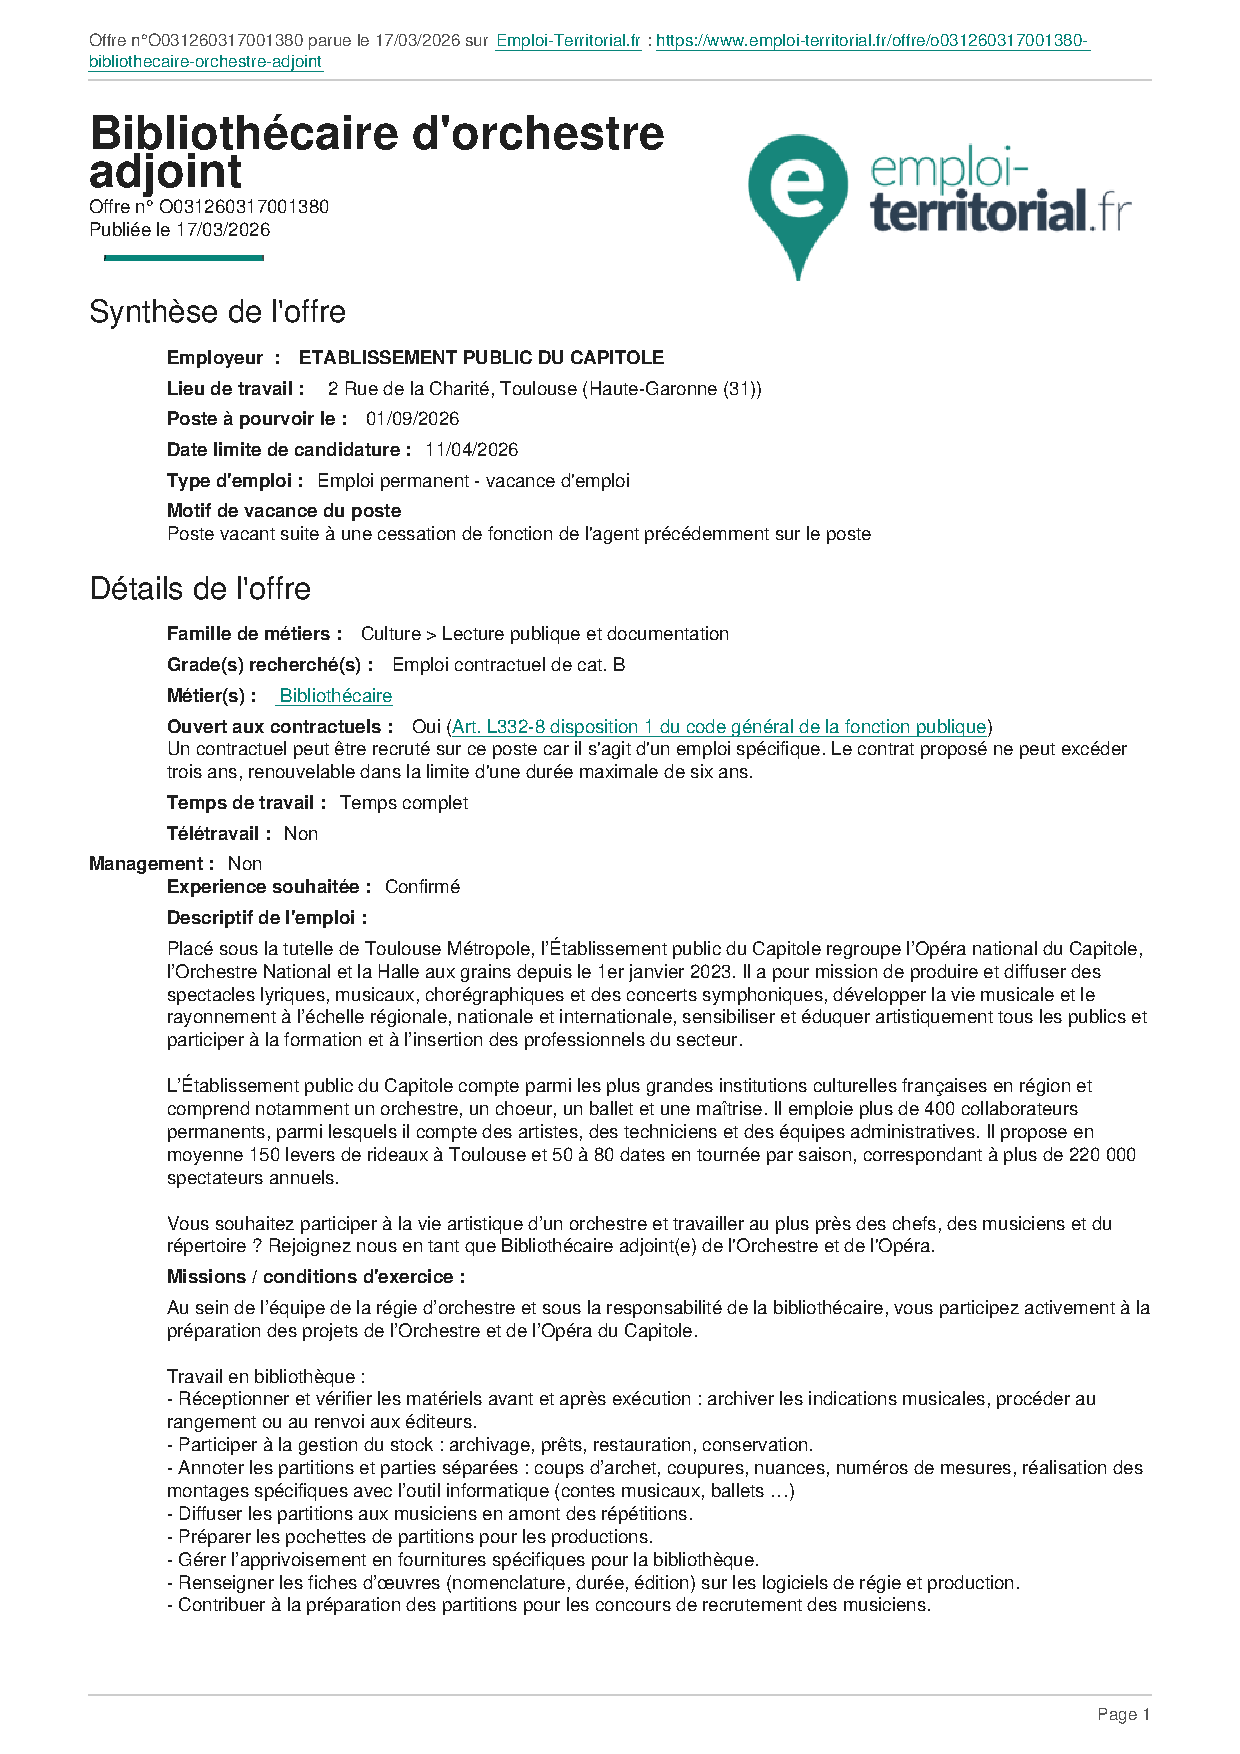
\includepdf
[pages=1-2, 
nup=2x1, 
landscape=true, 
scale=0.80, 
pagecommand={\subsection*{Fiche de poste de bibliothécaire musical à Toulouse}}]{annexes/annexe1toulouse.pdf}


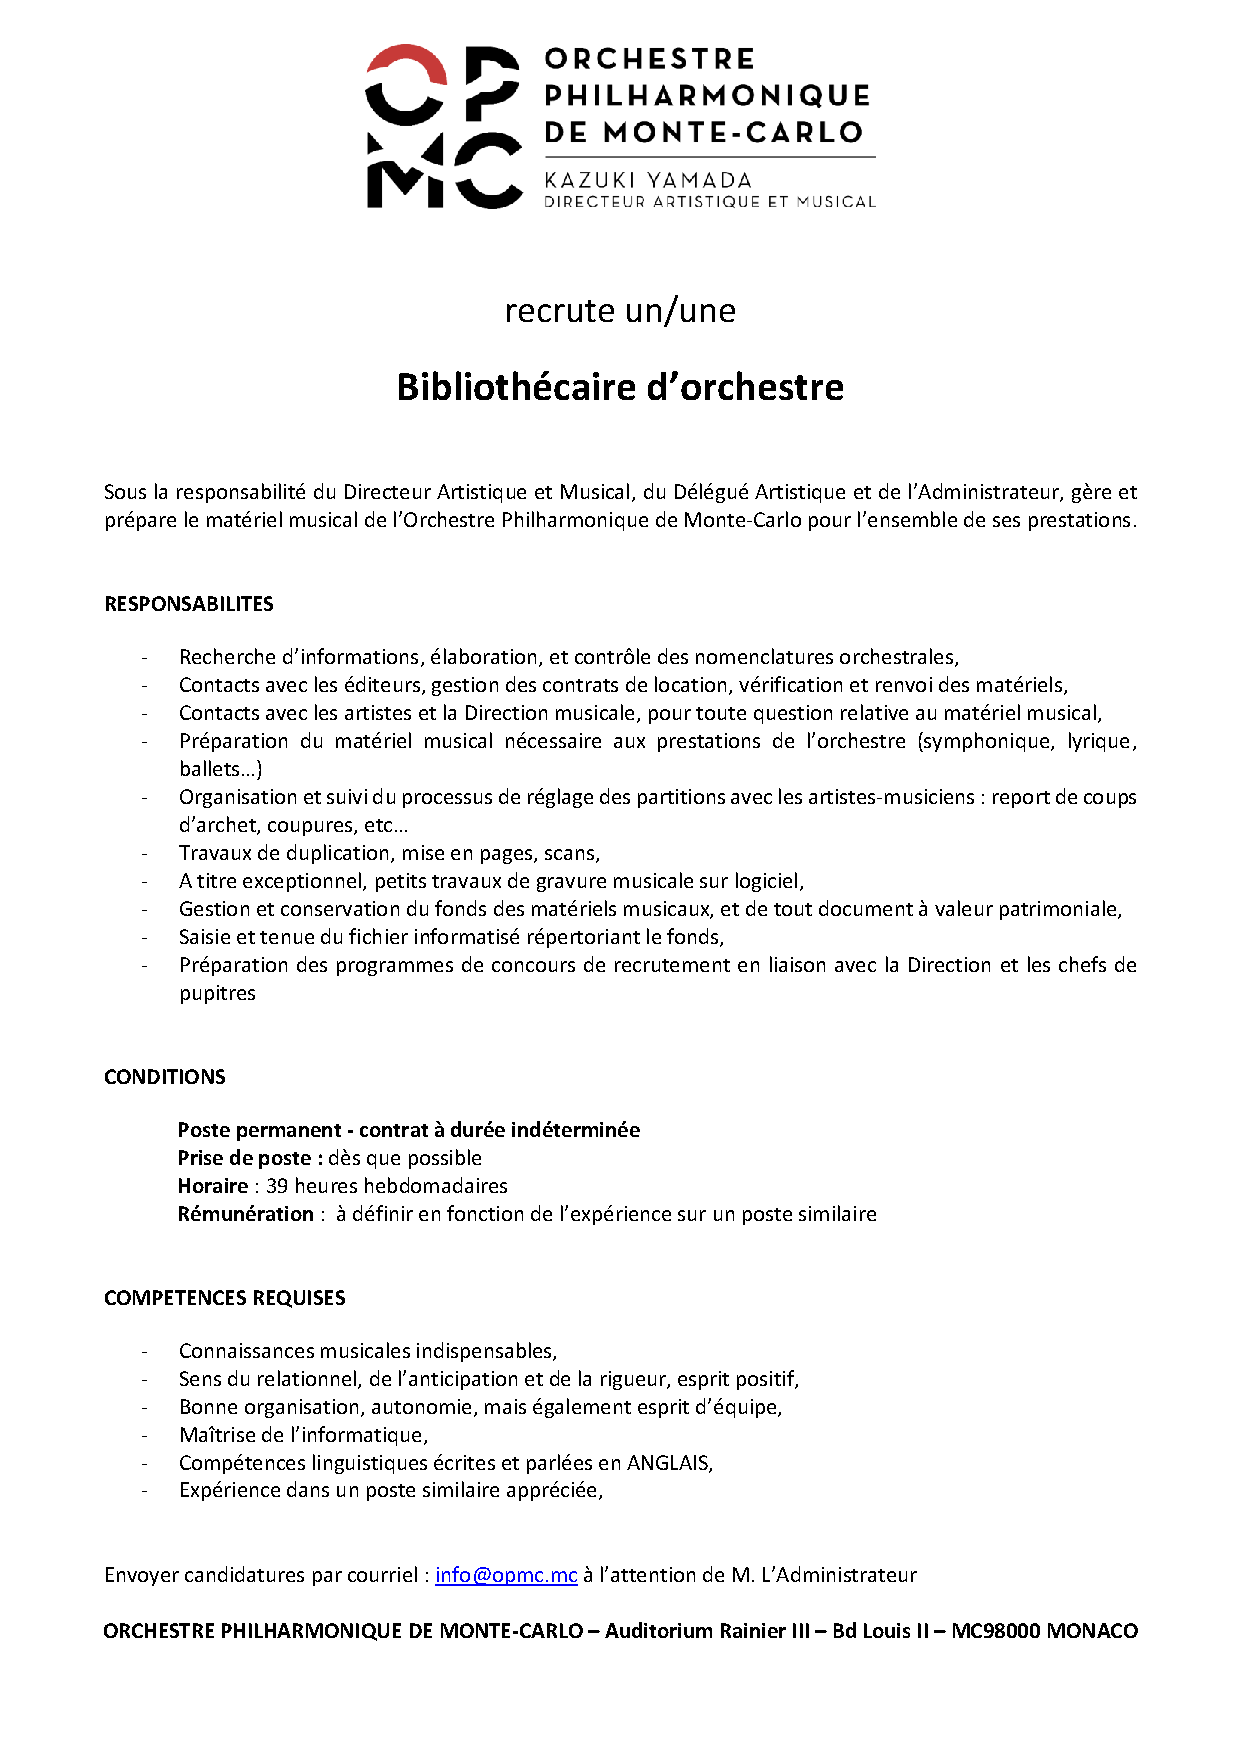
\includepdf
[pages={-},
scale=0.78,
pagecommand=\subsection*{Fiche de poste de bibliothécaire musical à Monte-Carlo}]{annexes/annexe2montecarlo.pdf}


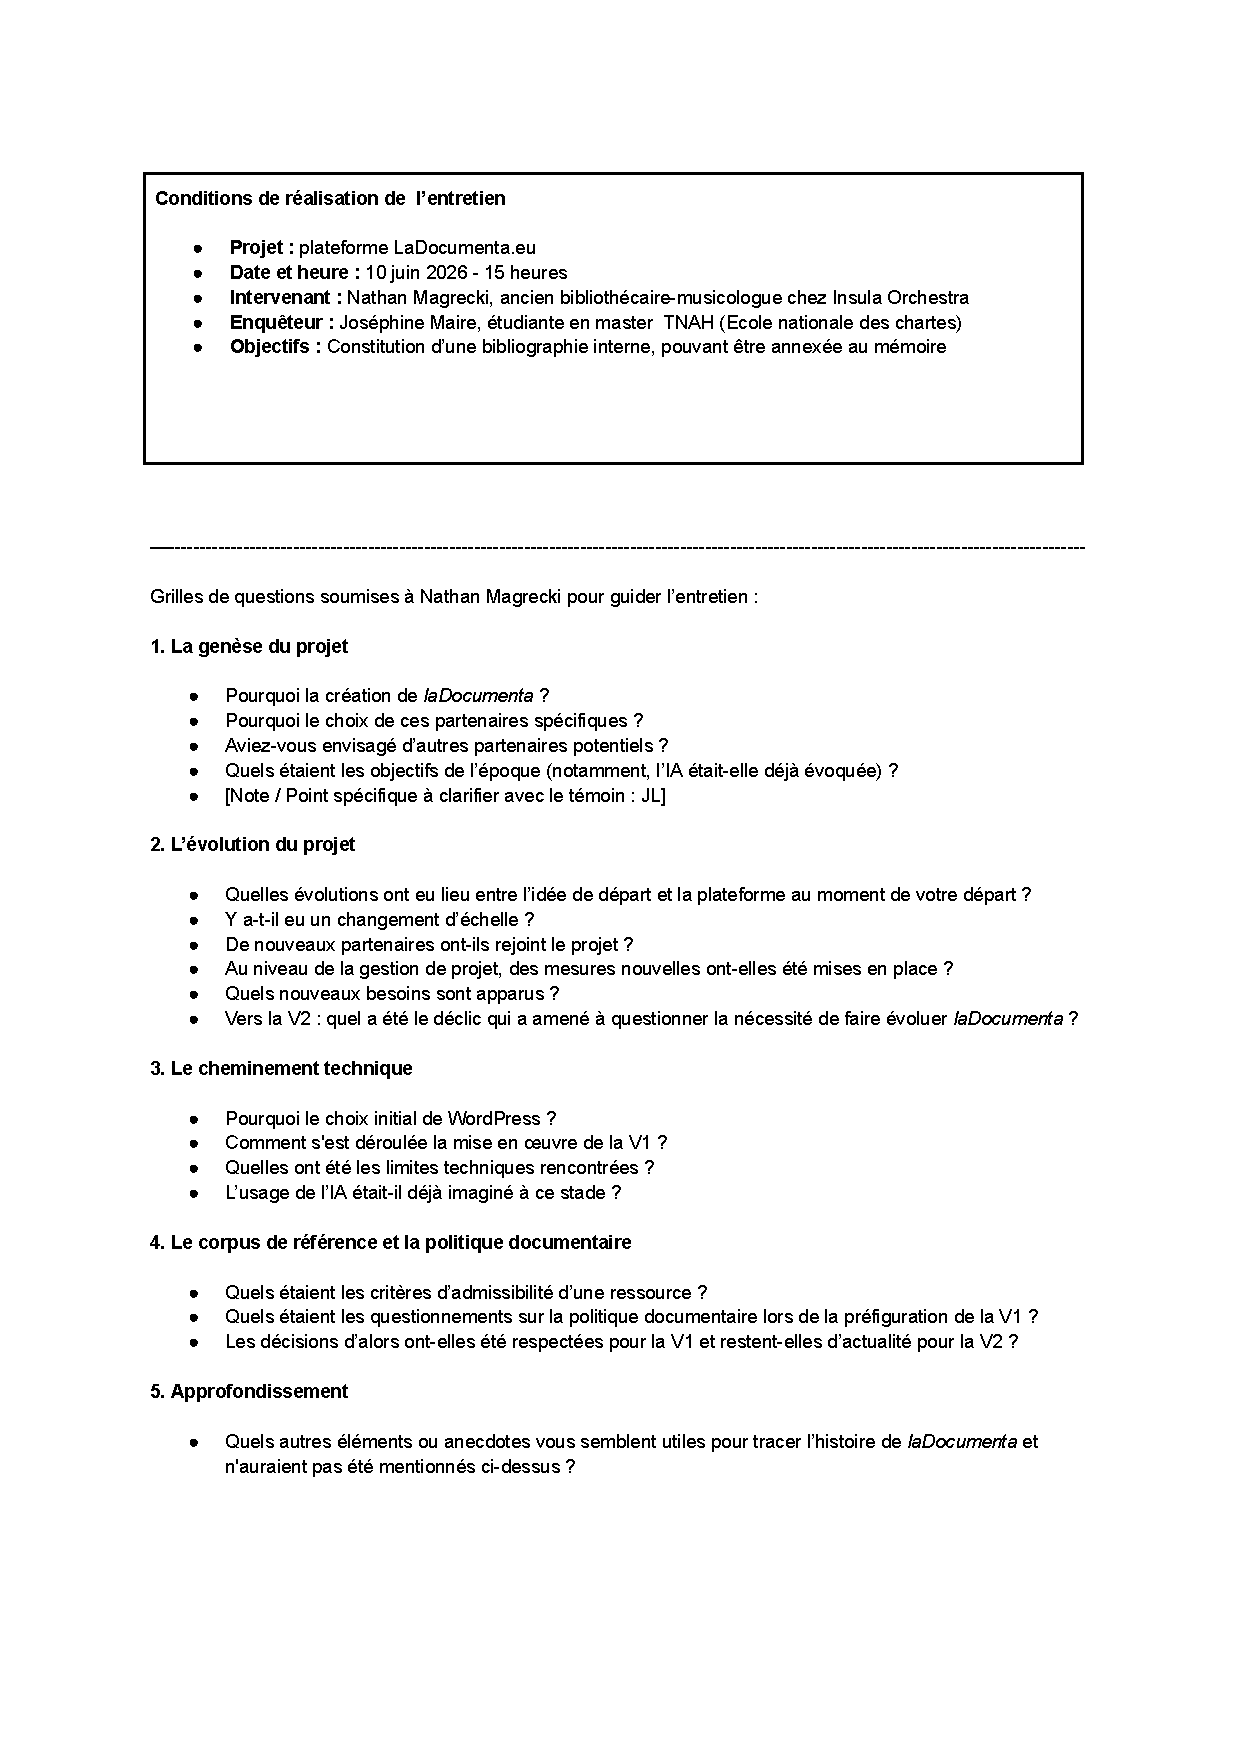
\includepdf
[pages={-},
scale=0.90,
pagecommand={\subsection*{Grille d'entretien : ancien bibliothécaire de LaDocumenta.eu}}]{annexes/annexe3entretienbibliothecaire.pdf}

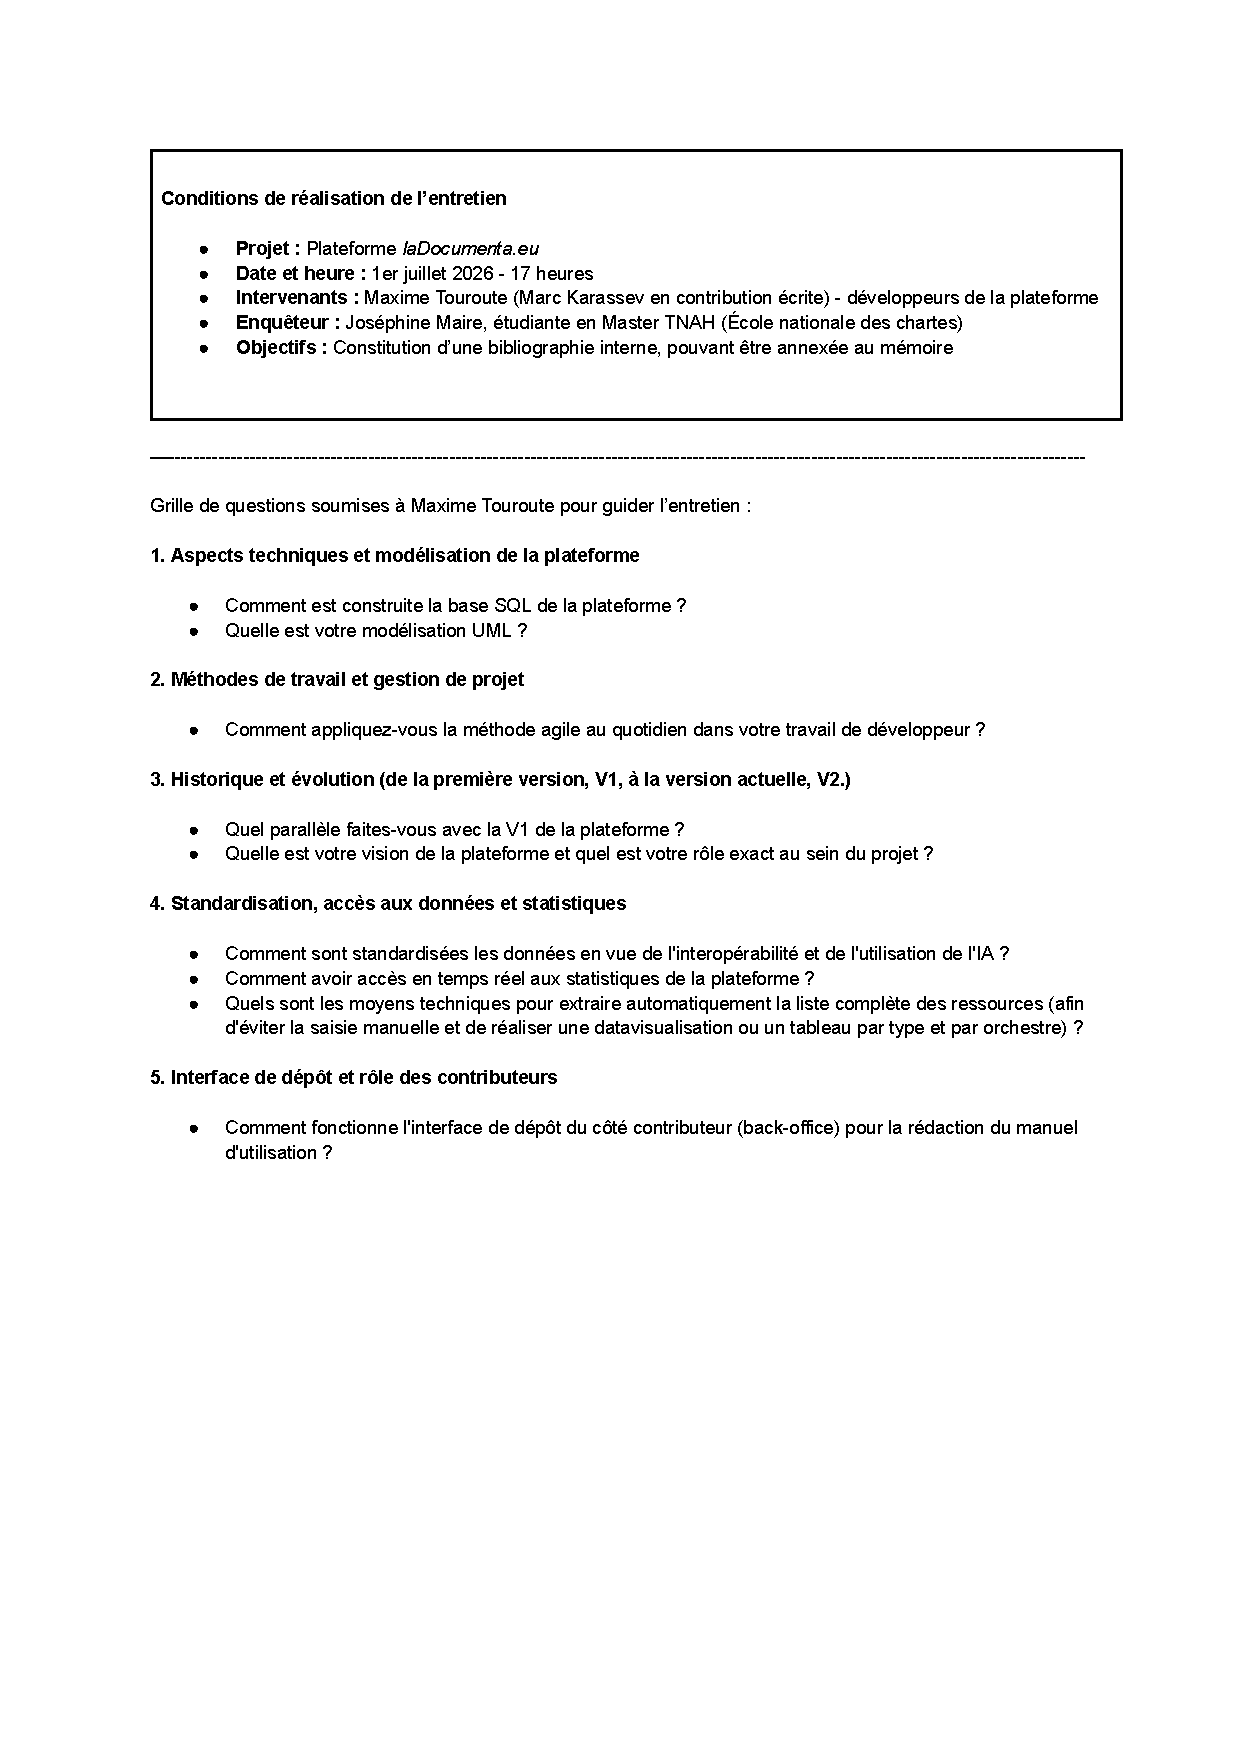
\includepdf[
pages={-},
scale=0.90,
pagecommand={\phantomsection\hypertarget{annexe:annexe4entretiendeveloppeur.pdf}{}\subsection*{Grille d'entretien : développeur de la plateforme LaDocumenta.eu}\label{annexe:annexe4entretiendeveloppeur.pdf}}
]{annexes/annexe4entretiendeveloppeur.pdf}


	
	%%%%%%%%%%%%%%%%%%
	
	\backmatter % glossaire, index, table des figures, table des matières.. (la bibliographie a déjà été appelée)
	
	%\printindex
	%\printglossaries[title=Glossaire]
	\listoftables
	\listoffigures
	\tableofcontents
\end{document}